% This is the official working version
% Last updated 2011 March 19

\documentclass[11pt,letterpaper]{spie}

\usepackage{natbib}
\usepackage{epsfig}
\usepackage{graphicx}
\usepackage{pgf}  
\usepackage{caption}
\usepackage{multirow}
%\usepackage{ctable}
\usepackage[normalem]{ulem}

\citestyle{aa}

%\oddsidemargin = 1.46cm
%\evensidemargin = 0.46cm
\topmargin = -0.1in
%\leftmargin = -1.0in
\textheight = 9.3 in
%\textwidth = 7.5in

\input macros % - Need this for journal abbreviations in the .bib file

\input latex_defs_ja

\input formatted_references 

\begin{document}
\mainbaseline

% -----------------------------------------------------------------------------

\newpage

\tableofcontents

\noindent{\it Note: As per the ROSES-2011 Solicitation NNH11ZDA001N
Appendix D.3 Section 1.2.2.3: Owing to the anticipated greater degree
of complexity, the scientific/technical/ management section of
proposals for a suborbital flight investigation may be 20 pages long
instead of the default 15 pages specified in the NASA Guidebook for
Proposers.}

\newpage

%\parskip0pt

%\citet{pober13baobab,pober13window,moore13,stefan13,parsons12a,parsons12b}

\pagenumbering{arabic}
\pagestyle{plain}

\section{Executive Summary}

\parskip0pt Understanding the formation and evolution of galaxies is
one of the foremost goals of astrophysics and cosmology
today.
The cosmic star formation rate has undergone a dramatic evolution of the course of the last seven billion years.  Dust-obscured star forming galaxies (DSFGs) offer the perfect tracers of this evolution as they contain much of the star-forming activity.
By their very nature, DSFGs are difficult to study and have, until recently, been poorly understood.
A variety of unextincted diagnostic lines are present in the far-infrared
(FIR) which can provide insight into the conditions of star
formation, including the instantaneous star formation rate, the effect of AGN feedback on star formation, the mass function of the stars, and the spectrum of their ionizing radiation.

Spectroscopy in the far-infrared is technically difficult but scientifically crucial, as underscored by the Decadal Review's endorsement of US involvement in the Japanese-led Space Infrared Telescope for Cosmology and Astrophysics (SPICA), a 4 K, 3 meter telescope optimized for FIR spectroscopy.  Involvement at the level of a complete NASA-funded instrument now seems unlikely in the current budgetary environment (though small critical hardware contributions are under consideration).  FIR spectroscopy from space-based platform with a cryogenic mirror can, in principle, achieve performance limited by astrophysical backgrounds.  However, we argue that stratospheric balloons offer a platform which can outperform current capabilities and are competitive against satellite missions for large area, spatial/spectral mapping. 
This is possible for a telescope using low-emissivity, high-throughput optics onto a dispersive spectrometer, and having high-sensitivity, large-format detector arrays.

We propose an aggressive program of instrumentation development and experimental study called the \namefull\ (\name), with the goal of demonstrating the key technical milestones necessary for balloon-borne FIR spectroscopy limited by the photon noise from the atmosphere. \name\ will address the two key technical issues necessary to achieve this:
\begin{enumerate}
\parskip-5pt
\item	Low emissivity, high throughput telescope and spectrometer optics 
\item	Background limited detectors in large format arrays, scalable to $>10^4$ pixels
\end{enumerate}
\parskip-5pt
We will do this by constructing an integral-field spectrometer from 240 - 420
\mum\ coupled to a \D\ off-axis telescope.  For the detectors, we will leverage the highly advanced development work of Jonas Zmuidzinas' group at Caltech / JPL on kinetic inductance detectors (KIDs).  KIDs represent the most promising route to economical, large format submillimeter detector arrays.  In addition to this technical demonstration, we will be able to obtain scientific results from \name\ from two North American overnight flights which will
\parskip-5pt
\begin{enumerate}
\parskip-5pt

\item \label{goal:Lines} Obtain spectra of $\sim100$ galaxies in the fine structure lines \cii(157 \mum) ($0.5 < z < 1.54$), and for lensed galaxies, \oi(63 \mum), and \oiii(88 \mum) ($2 < z < 4$)

\item \label{goal:PowerSpectrum} Demonstrate deep tomographic maps capable of detecting the shot noise power spectrum of \cii\ at $z\sim1$

\end{enumerate}
\parskip-5pt
With these goals met, it is our explicit intention to build upon this proposal in order to successfully propose a wholly unprecedented experiment to study the cosmic star formation history.  This future experiment will make a 3-D cube spanning spanning at once at least 4 billion years of
cosmic history ($0.5 < z < 1.5$), on scales from 1 - 50 Mpc (30\arcsec\ to $>1\arcdeg$) with complete spectroscopic
information.   This would be done with fully three dimensional tomographic maps
of emission in \cii\ and other lines.
Such an experiment fills a unique and vital scientific niche not filled by \herschel, SOFIA, ALMA, or even SPICA.

% from the unobscured ionized carbon fine structure line
% \cii(157.7 \mum,) 
% The total cost for a
% 5-year program to build, fly, and analyze the data from \icaris\ was \$6.84M.  
% Though this proposal was very highly ranked, it was not funded.  

% 
% 
% 
% \name\ will retain the telescope aperture (2.5 meter) and total spectral coverage (240 - 420 \mum) as \icaris, but we have reduced costs by reducing the flight program to two North American flights (instead of an LDB flight), and reducing the instantaneous spectral coverage to half (with the full range covered by scanning the diffraction grating). 
\parskip0pt


%can be extended to LDB with longer hold-time cryostat 




%In addition, we will characterize the atmospheric emissivity beyond the purely %theoretical models currently available.  


We stress that much of the work for \name, including the telescope and spectrometer optics, detectors, and detector readout, can be directly re-used in a future experiment. The frequency domain RF readout of KIDs is relatively inexpensive per pixel, and highly scalable, and the detectors themselves can be swapped out while maintaining the same readout.  We note there is still is significant discovery potential with \name, since it will be probing an under-explored wavelength range with unprecedented sensitivity.


% The key
% science goals of \icaris\ are:
% 
% \parskip-5pt
% \begin{enumerate}
% \parskip-5pt
% 
% \item 
% \label{goal:LCII-LFIR}
% {\bf Thoroughly characterize the relation in galaxies between star
% formation rate (SFR), \cii\ luminosity ($L_{CII}$), and far-infrared
% (FIR) luminosity $L_{FIR}$ over the range $10^{11} < L_{FIR} < 10^{13}$
% for redshifts $0.5 < z < 1.5$.}  \herschel-PACS and SPIRE have
% provided numerous measurements of \cii\ (and other far-IR lines) in
% nearby galaxies, and optical surveys
% %(comprising $\sim 10^6$
% %galaxies at low $z$ and $10^5$ at $z\sim1$) 
% ave characterized the redshift evolution and star formation of the
% unextincted galaxy population.  Thus $0.5 < z < 1.5$ is the key range
% to overlap a survey of dust-extincted galaxies with the well-studied
% optical population, and extend what is known about dusty star
% formation from the local population.  \icaris\ will detect $\sim100$
% individual galaxies in the \cii\ line at $>5\sigma$ significance down
% to a limiting galaxy FIR luminosity of $1.4 \times 10^{12}$~\Lsun\ at
% $z=0.5$ ($3.2 \times 10^{12}$~\Lsun\ at $z=1.5$), and several thousand
% at lower significance.  Because we will survey fields with rich
% multi-wavelength coverage, including continuum photometry from the
% optical to the sub-mm and spectroscopic optical redshift surveys
% containing a wealth of other star-formation indicators, we will also
% be able to accurately locate and stack lower significance detections
% within the data cube, obtaining an average relation between \cii\
% luminosity and SFR as a function of galaxy type and redshift.  This
% combined information will calibrate the \cii\ line against other
% star-formation indicators as a function of galaxy luminosity and
% redshift.  Combined with existing data, we will characterize the rate,
% efficiency, mode, extent and timescale of star formation.
% %  By
% %constraining the star formation rate, we will also be able to
% %determine the relative importance of AGN and starbursts in producing
% %the galaxy luminosity.
% %This will allow us to
% %use \cii\ luminosity as a star formation indicator, thereby making a
% %``\cii\ Madau plot''.  
% No existing facility will be as effective in measuring dust-obscured
% star formation over this range in luminosity and redshift.
% \parskip-5pt
% \item 
% \label{goal:PowerSpectrum}
% {\bf Measure the environmental dependence of dusty star-formation from
% $0.5 < z < 1.5$ to complement studies at $z < 0.3$ with SDSS via the
% power spectrum of \cii.}  The three dimensional power spectrum of
% galaxies provides the best measure of their relation to the underlying
% dark matter potential.  By producing a redshift survey, \icaris\ can
% measure the clustering of dusty galaxies -- and thereby constrain
% models of galaxy formation -- far better than previous surveys which
% measure the angular power spectrum or rely on photometric redshifts.
% In addition to the power spectrum of \cii, we will also be able to
% measure the cross-correlation with the emission of \nii(122 \mum),
% \nii(205 \mum) and \oi(145 \mum), which will serve both as a guard
% against systematic contamination, and also provide statistical
% information on the evolution of these line ratios with redshift and
% environment.  \icaris\ is designed so that this power spectrum
% measurement can be made with high significance.  Once demonstrated,
% this ``intensity mapping'' will become a powerful technique or future
% observations with SPICA, as well as ground based instruments like
% those envisioned for CCAT.
% \end{enumerate}
% \parskip-11pt
% 
% We stress that there is significant discovery potential with \icaris,
% since it will be probing an under-explored wavelength range with
% unprecedented sensitivity.

\clearpage

\parskip0pt
\section{Relevance to NASA Objectives}

\name\ advances NASA's strategic scientific and technical goals in a
wide variety of ways.  Broadly, \name\ supports Goal 2 of the NASA
2011 Strategic Plan to ``Expand scientific understanding of the Earth
and the universe which we live'', specifically addressing sub-goal 2.4
to ``discover how the universe works and explore how it began and
evolved''. The proposal is relevant to NASA's 2007 Science Plan in
addressing the Science Question: ``How do planets, stars, galaxies, and
cosmic structure come into being?''

\begin{itemize}
\parskip-11pt

\item
\name\ takes the next leap in our understanding of the universe by
moving from far-IR imaging to far-IR spectroscopy with an order of
magnitude improvement in current capabilities.  \herschel\ will soon
be exhausted of cryogens, and ALMA Band 9 (420 -- 500 \mum) is just
coming online.  \name\ will cover the spectral range 240 \mum - 420
\mum, bridging the gap between \herschel-PACS and ALMA Band 9, a
wavelength range nearly completely inaccessible from the
ground\footnote{Note that ALMA Band 10 (787 - 950 GHz; 320 - 380 \mum)
will have overlap with \name, but this will be one of the last bands
completed and the most sensitive to weather.}.  \name\ will have
sensitivity to extragalactic spectra more than an order of magnitude
greater than the {\em Herschel}-SPIRE FTS (in their region of spectral
overlap), and will be significantly more sensitive than any instrument
on SOFIA for extragalactic sources; see Figure \ref{fig:SensCompare}.  \name\ observations will
provide new data not available from existing facilities to complement
the X-ray to radio data from satellites (\chandra, \xmm, \hst,
\spitzer, \herschel, \planck, \akari), airborne (SOFIA) and
ground-based telescopes (Gemini, Subaru, VLT, UKIRT, VISTA, Keck)
participating in the NASA ORIGINS program.
\parskip-5pt
\item
\name\ addresses the objectives of the APRA solicitation by
developing a significant new suborbital platform for submillimeter
astronomy, and by dramatically advancing the state-of-the-art in
detectors for submillimeter wavelengths.  \name\ will have the
largest number (6000) of the most sensitive far-infrared 
detectors ever fielded in a scientific instrument.  This technical
development
% of a significant new suborbital platform for
%submillimeter astronomy and the fielding of the largest number (6144)
%of the state-of-the-art bolometer detectors in a scientific instrument
supports Goal 3 of the NASA 2011 Strategic Plan to ``Create the
innovative new space technologies for exploration, science, and
economic future''.  Specifically, the \name\ program will ``develop
and demonstrate the critical technologies that will make NASA's
exploration, science, and discovery missions more affordable and more
capable'' (Sub-goal 3.3).  This applies to future suborbital missions.
Our team has developed and is maintaining significant infrastructure
of attitude determination and control that is being exploited by a
variety of balloon payloads including EBEX, SPIDER, InFOC$\mu$S, and
HEFT.  The \name\ telescope is designed with a wide field of view
and a generic placement for the receiver, making it very
flexible and re-usable, allowing us to easily place
upgrades to the \name\ spectrometer or new prototype submillimeter
receivers there.

\item
\name\ will train the next generation of astrophysicists, from undergraduate and graduate students to postdoctoral
fellows.  This supports Goal 6 of the NASA 2011 Strategic Plan
to ``Share NASA with the public, educators, and students to provide
opportunities to participate in our Mission, foster innovation, and
contribute to a strong national economy''. Our previous sub-orbital
sub-millimeter astronomy experiment \blast\ produced eight Ph.D's and
trained several postdocs.  It also led to a public documentary film
{\em BLAST!} \footnote{\tt http://www.devlinpix.com/film/blast} which
supported subgoal 6.4 of the NASA Strategic Plan to ``Inform, engage,
and inspire the public by sharing NASA's missions, challenges, and
results''.  \blast\ also involved over a dozen undergraduates who
built hardware, designed parts, and participated in the analysis.  For
graduate students, suborbital program is the perfect place to learn
how to do astrophysics end-to-end, from experimental design to
instrument construction to data analysis to theoretical
interpretation.  \name\ will lead to similar achievements on the
educational front over the next 5 years, specifically addressing
(sub-goal 6.1) to ``improve retention of students in STEM disciplines
by providing opportunities and activities along the full length of the
education pipeline.''

% \item
% \name\ complements the future NASA missions JWST and WFIRST and
% joint NASA missions with international partners Euclid and SPICA.
% \name\ will probe the ensemble properties of star-forming galaxies at
% the peak epoch of the star-formation history of the universe that JWST
% seeks to characterize individually.  
% A NASA-contributed instrument on
% SPICA can make very deep spectroscopic measurements of the $z\sim1$
% galaxies at mid and far-IR wavelengths, depending on the final choice
% of instruments and survey strategy.  The importance of space-based
% far-infrared spectroscopy was supported by the ASTRO2010 Decadal
% Survey (see the white papers by
% \Citet{appelton09,stacey09}\footnote{Throughout the proposal, we
% indicate published work done by members of the proposing collaboration
% in bold face.}).  \name\ could motivate an all-sky space-borne
% spectroscopic shallow surveyor at far-IR wavelengths to complement a
% ground-based experiment such as CCAT and a space-based observatory
% such as SPICA, similar to WISE/Spitzer complementarity.

\end{itemize}

\begin{figure}[h]
  \begin{tabular}{ll}
    \begin{minipage}{3.25in}
      \begin{center}
	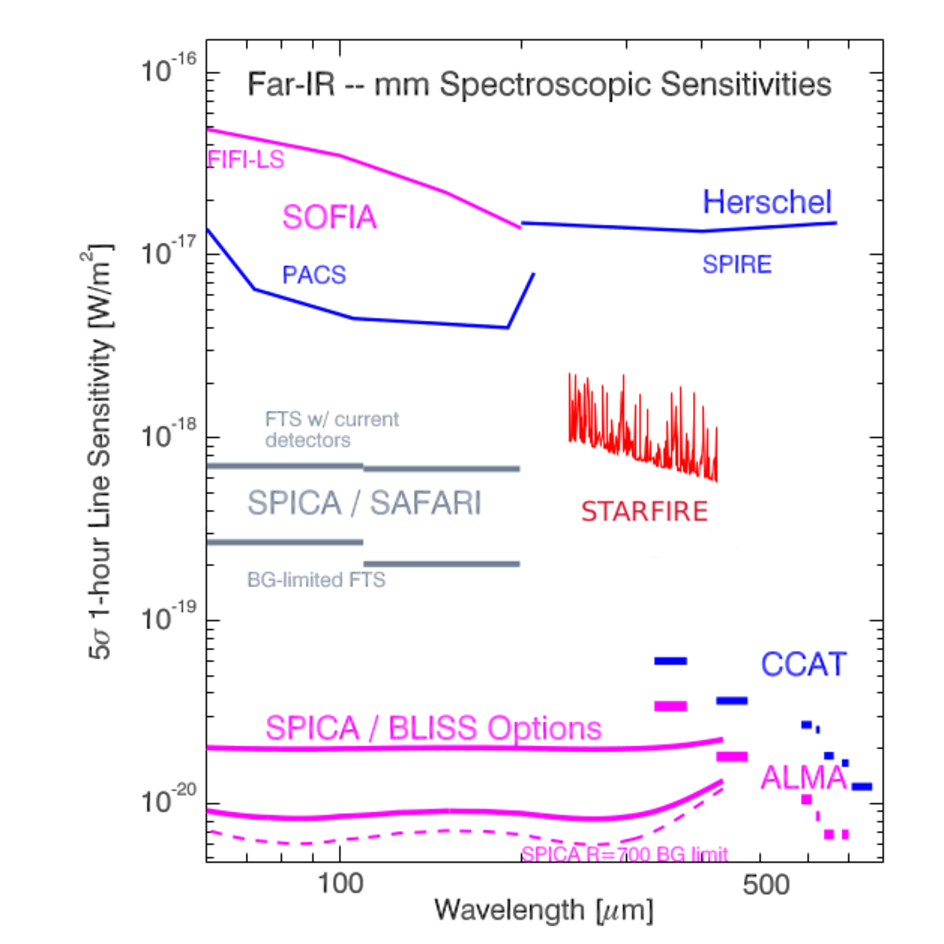
\includegraphics[height=3in]{sensitivity_2012.pdf}
      \end{center}
    \end{minipage} &
    \begin{minipage}{3.25in}
      \begin{center}
	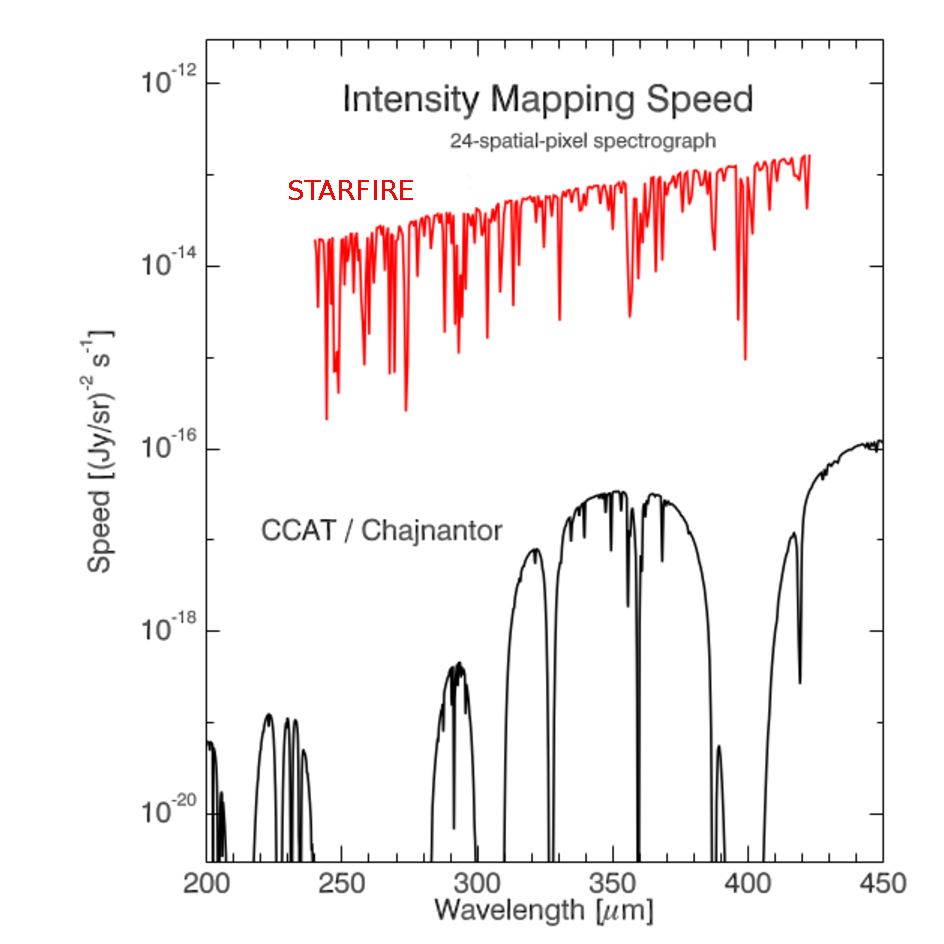
\includegraphics[height=3in]{icaris_nei.pdf}
      \end{center}
    \end{minipage}
  \end{tabular}
      \captionbaseline\caption{\small \L\ \name\ (red) compared to current and
	future spectroscopic instruments.  We compute a $5\sigma$ 1
	hour sensitivity on a single source as the benchmark. The
	variation in the \name\ sensitivity is due to atmospheric
	emission lines.  Approximately 10\% of the band is compromised
	due to these lines, though they may still be used for
	frequency calibration. \R\ The mapping speed of \name\
	compared to an identical instrument on CCAT.  Here larger
	values correspond to more area mapped to the same depth in the
	same time; a balloon instrument like \name\ is as much as 3 orders of magnitude
	faster.  Note that for intensity mapping, telescope area is
	not a factor.  Note also the significant regions in redshift
	not accessible from the ground even at the best sites.}
      \label{fig:SensCompare}
\end{figure}

%\clearpage






















\section{Scientific Program}

\subsection{Background}

\subsubsection{History of Star Formation}

The detailed story of the formation of galaxies within a cosmological
framework is a major unsolved problem in contemporary cosmology
\citep[see, e.g., the recent review by][]{benson10}.  Between the end
of reionization and about 8 Gyr after the Bang, the cosmic star
formation rate density rises steadily, reaching a peak at $z\sim2.5$;
see Figure \ref{fig:ScienceCase}.  The nature of the star-forming
systems changes dramatically over this period, with the most luminous
galaxies at the peak becoming heavily dust enshrouded.  Indeed, the
discovery of the cosmic far-infrared background (CFIRB) by NASA's
\cobe\ satellite \citep{puget96,fixsen98} and the detection of a
significant population of high redshift, dust-obscured galaxies
selected at submillimeter (submm) wavelengths \citep{smail97,hughes98}
revealed that as much as half of the star formation activity in the
early Universe occurs in galaxies that are undetected at optical
wavelengths \citep{chapman05,aretxaga07}.

\begin{figure}[h]
  \begin{tabular}{ll}
    \begin{minipage}{3.25in}
      \begin{center}
	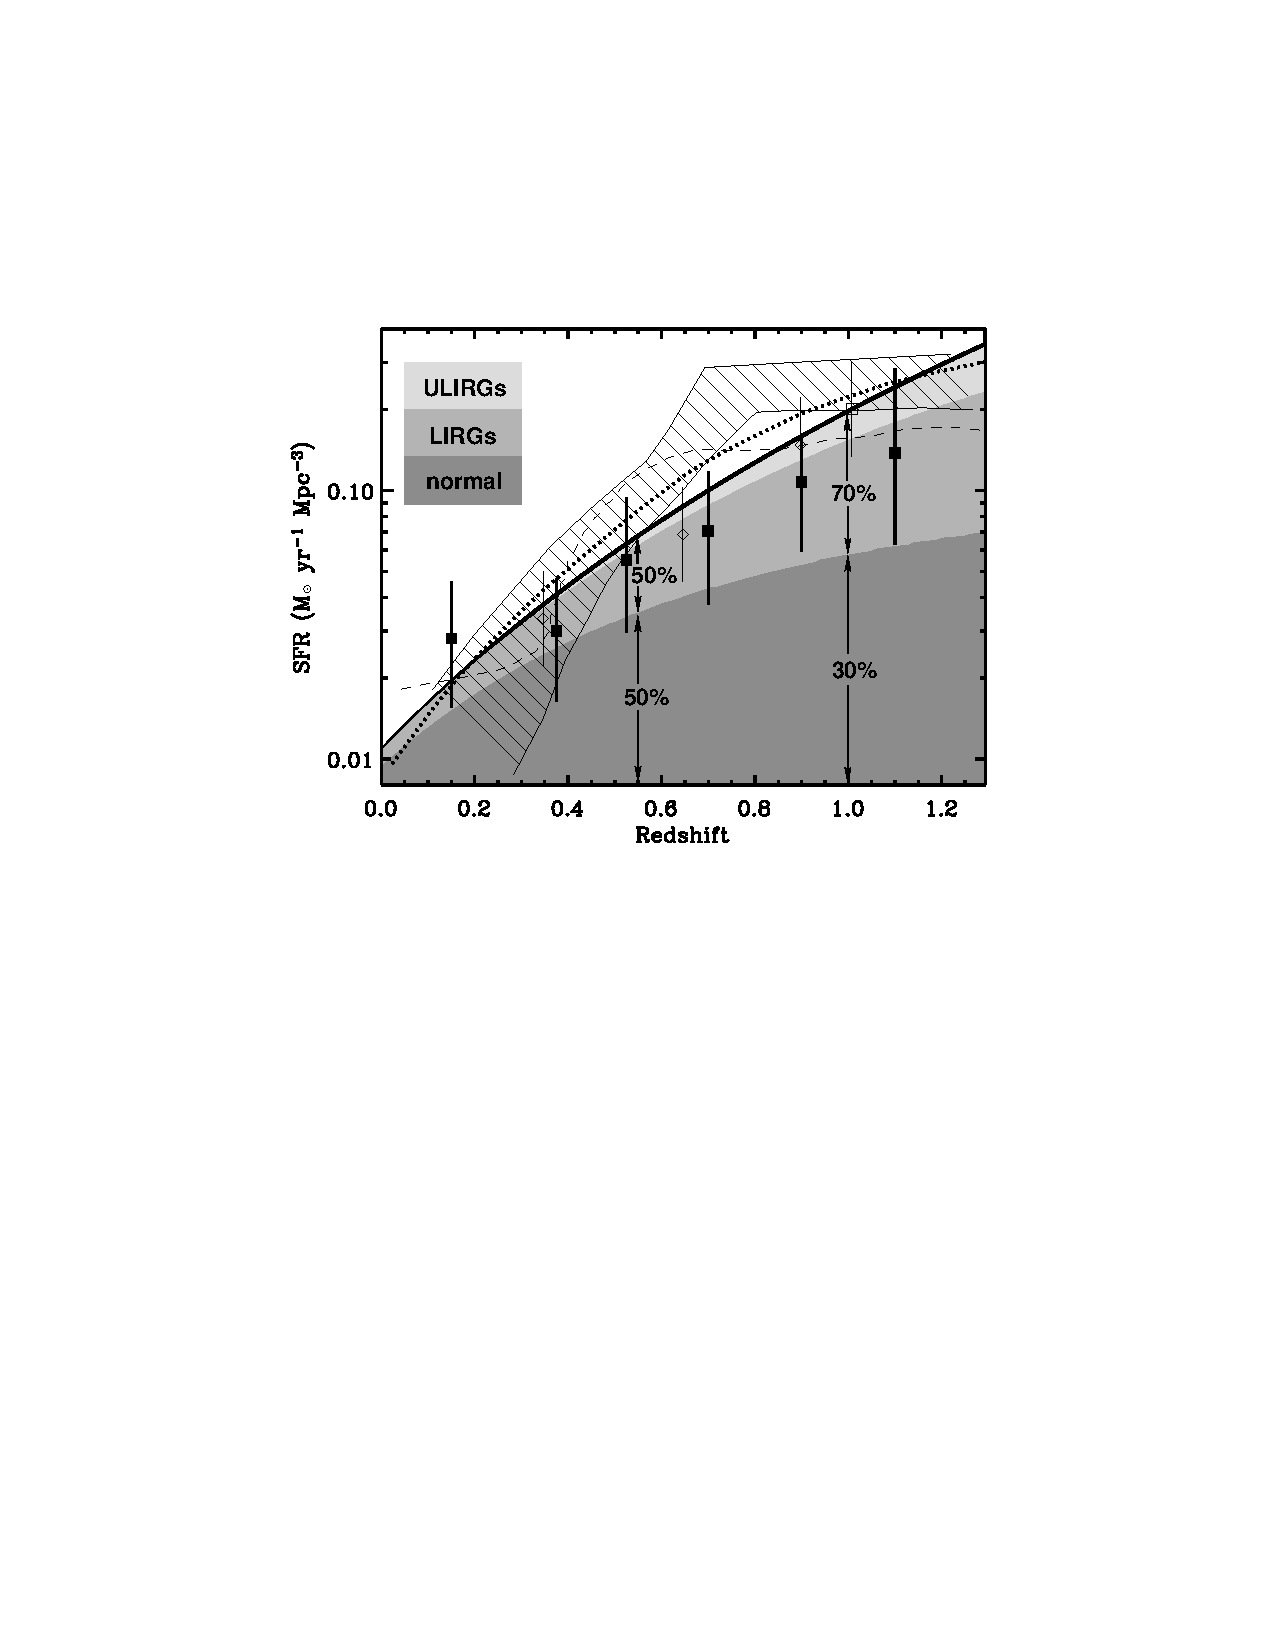
\includegraphics[width=3.25in]{lefloch04_sf_history.pdf}
%{madau_plot_somerville08.pdf}
      \end{center}     
    \end{minipage} &
    \begin{minipage}{3.25in}
      \begin{center}
	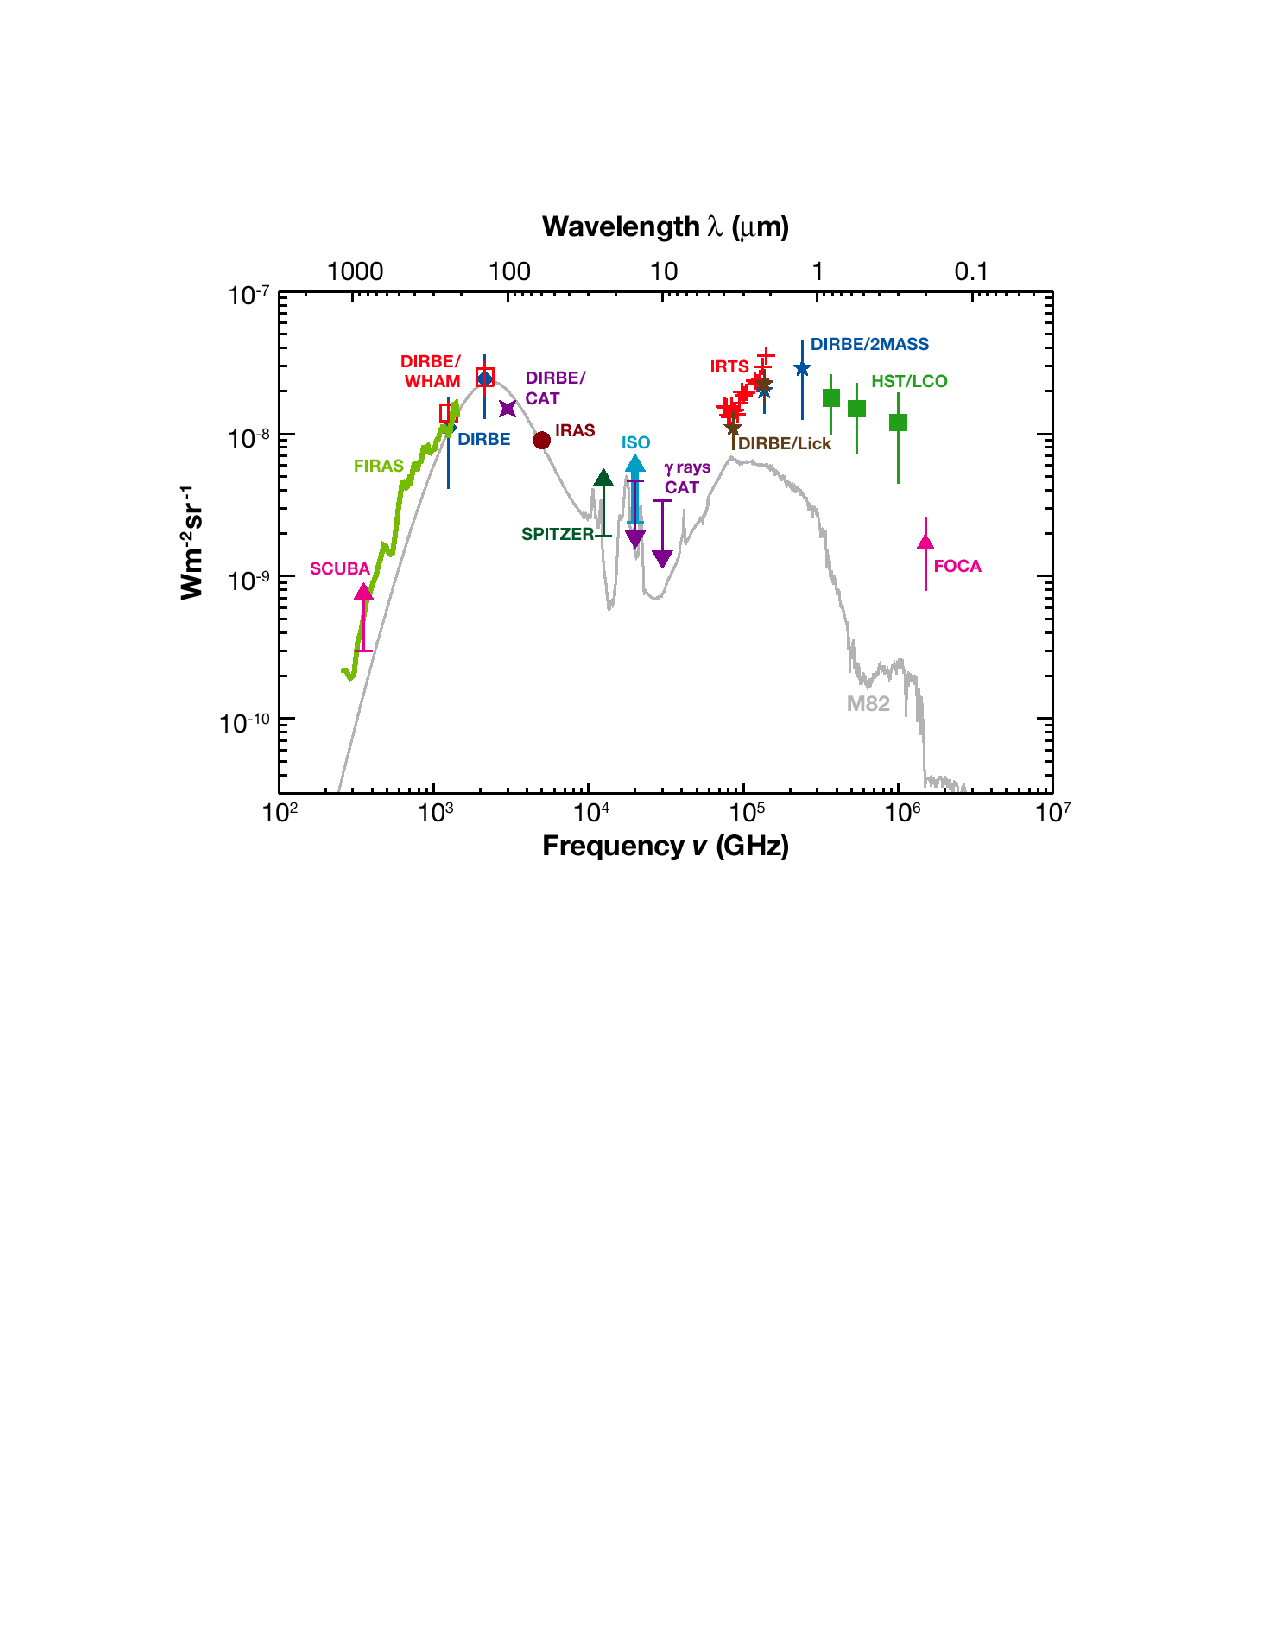
\includegraphics[width=3.25in]{lagache05_firb.pdf}
      \end{center}
    \end{minipage}
  \end{tabular}
	\captionbaseline\caption {\small {\it Left:} The evolution cosmic star
	formation rate density, broken down by the contributing
	population, from \citet{lefloch04}. {\it Right:} The fraction
	of extra-galactic background light due to far-infrared sources
	\citep{lagache05}.  Note that roughly equal amounts come from
	the optical/near-IR and far-IR.  Of the far-IR, about half the
	intensity lies at $z<1$.}
	\label{fig:ScienceCase}
\end{figure}

These (sub)millimeter-selected galaxies (hereafter SMGs) which
comprise the CFIRB are a cosmologically significant population
undergoing intense star formation (with star formation rates of up to
$\sim10^3$~M$_{\odot}$~yr$^{-1}$) when the Universe was \mbox{15 -
45\%} of its present age, between 7.5 and 11.5 billion years
ago. Optical and ultraviolet (UV) radiation from both star formation
and AGN activity heat the dust in these galaxies, and this energy is
thermally re-radiated at far-infrared (far-IR) to mm wavelengths, with
the peak of dust emission occurring at $\sim60-200\,\mu$m in the
rest-frame \citep{soifer91}.  The large amount of dust present in them
often precludes detailed study at optical wavelengths.

Most studies suggest that the far-IR populations have had a different
energy release history from the optically-selected populations, which
appear to have experienced a more constant rate of energy release with
cosmic time (e.g. \citet{hopkins07}).  Further, even for the subset of
dusty galaxies for which optical counterparts can be identified and
optical spectra obtained, the high obscuration ensures that the
optical spectra do not probe the bulk activity in these
galaxies. \citet{goldader02} and others have demonstrated this,
showing that luminosities based on UV/blue fluxes and colors
underestimate the total luminosities of a sample of LIRGs and ULIRGs
by factors of 3--75, and that the UV/optical light often comes from
regions hundreds of parsecs from the true luminosity sources.

SMGs are thought to mark the formation of the massive elliptical
galaxies seen in the local universe \citep{swinbank08}. The molecular
gas masses implied by $^{12}$CO measurements of typical SMGs are
$\sim10^{10-11} M_{\solar}$; given their inferred star formation
rates, this implies that SMGs could have built up all of the stellar
mass in spiral bulges or massive elliptical galaxies in a burst of
$10^8$ years duration \citep{smail02,swinbank04}.  SMGs have been
shown to reside in the most massive dark matter halos at $z\sim2.5$
\citep{blain04,amblard11}.  Clustering has been measured for
\herschel\ sources, with a distinction detectable between the
contributions to clustering from one- and two-halo terms in the models
\Citep{cooray10}.%; see Figure \ref{fig:Clustering}.

This population has evolved strongly over the last half of the
Universe's life.  The Spitzer 24~\mm-selected sources confirm a
dramatic decrease in far-infrared luminosity from $z\sim1$ to the
present: \citet{lefloch05} infer a shift in characteristic luminosity
$L^*$ at a rate of $(1+z)^{4.0\pm0.5}$.  Recent results from \blast\
\Citep{devlin09} and \herschel\ \citep{bethermin12} confirm that about
half of the CFIRB was created at $z<1$.

\parskip0pt



%\begin{figure}[h]
%  \begin{tabular}{lll}
%    \begin{minipage}{2.15in}
%      \begin{center}
%	\includegraphics[width=2.15in]{cooray_clustering_250.pdf}
%      \end{center}     
%    \end{minipage} &
%    \begin{minipage}{2.15in}
%      \begin{center}
%	\includegraphics[width=2.15in]{cooray_clustering_350.pdf}
%      \end{center}
%    \end{minipage} &
%    \begin{minipage}{2.15in}
%      \begin{center}
%	\includegraphics[width=2.15in]{cooray_clustering_500.pdf}
%      \end{center}
%    \end{minipage}
%  \end{tabular}
%	\caption {\small {\it Left:} The clustering of galaxies in the
%	HerMES survey at 250, 350 and 500 \mum\ from \citet{cooray10}.
%	Note that the functions measured are angular correlations (in
%	real space).  Dotted lines indicate the underlying one- and
%	two-halo terms in the model fit.  A marginal detection of the
%	crossover is made.}
%	\label{fig:Clustering}
%\end{figure}
%
\subsubsection{Astrophysics of \cii}

The ultraviolet radiation from newly-formed high-mass stars within
molecular clouds strongly affects the natal molecular interstellar
medium (ISM).  Within the immediate stellar vicinity, hydrogen is
fully ionized, forming an H{\small II} region whose size is set by
cloud density and the number of H ionizing (Lyman continuum) photons
that are available. Just beyond the H{\small II} region, far-UV (6
eV~$< h\nu <$~13.6 eV) photons penetrate the neutral gas where they
photoionize atoms and photo-dissociate molecules with ionization or
dissociation potentials less than 13.6 eV, forming photodissociation
regions (PDRs). The far-UV field strength $G$ is parametrized in
units of the local far-UV radiation field, $G_0=1.6 \times 10^{-3}\rm
erg\, s^{-1}\,cm^{-2}$.

PDRs are an important ISM component: typically 10\% by mass in normal
Milky-Way-like galaxies, but up to 50\% in starbursting nuclei of LIRG
and ULIRG galaxies that produce the infrared background.  The heating
of gas in PDRs is primarily through the photo-electric ejection of
energetic electrons from grains, with typical efficiency $\sim 1\%$.
After gas excitation and dissociation, most of the remaining stellar
energy goes into heating dust grains, which re-emit the energy in the
far-IR continuum (e.g. \cite{tielens85}).  Thus, on small scales where
the emitting region is resolved, the far-IR intensity should equal the
inferred UV intensity $G$.  For unresolved galaxies, the ratio of the
observed far-IR continuum flux to inferred $G$ is the beam filling
factor, or equivalently the physical size of the starburst region in
kpc$^2$.

\cii\ is particularly interesting, as it is a primary coolant of these
dense PDRs, as well as moderate density ``atomic clouds''.  It is very
luminous, typically the brightest gas-phase feature emitted by
galaxies, with up to 1\% of the total far-IR luminosity.  The
measurement of \cii\ intensities alone provides important insights
into star formation.  The \cii/far-IR continuum luminosity ratio, $f$,
measures the strength and spatial extent of the starburst.  $f$ is
strongly inversely proportional to UV field strength $G$ for
$G\sim10^1$ to $10^4$, maximizing at ~1\% for $G\sim$10 and $n\sim
10^3\rm\,cm^{-3}$.  The inverse relation occurs because the efficiency
of photoelectric heating is reduced at high $G$ due to the build-up of
grain charge, and because of the increased gas cooling via the \oi\ 63
\mum\ line. Therefore, within these ranges for $G$ and $n$, the
measurement of $f$ determines $G$.

\Citet{stacey10} recently obtained new measurements of \cii\ in 13
sources with $1 < z < 2$ (including a previous detection in
\Citet{hailey-dunsheath10}).  These starburst dominated systems have
$f\sim3.1\times10^{-3}$ while the AGN dominated systems have
$f\sim3.3\times10^{-4}$.  Thus $f$ appears to pick out star formation
dominated systems.  This survey also showed that, unlike local
starbursts and ULIRGS, where starbursts are confined to 100's of pc
scales, starbursts at $1 < z < 2$ extend over few kpc scales.  They
also have FUV fields like those found in M82 ($G\sim1000$)-- not the
super intense fields found in local ULIRGs ($G>10^4$).  This is
important as it suggests that local ULIRGs are a poor model for the
super starbursts at $1 < z < 2$ and expectations about $f$ based on
local systems \citep[e.g.][]{curran09,luhman03} should be informed by
more data.

Obtaining \cii\ fluxes and continuum measurements permits the
measurement of the star formation rate and spatial extent of the
starburst in the galaxy, measurements which cannot be done optically.
For the brightest objects, star formation rates obtained in this way
can be calibrated with multi-wavelength data and unconfused submm
SEDs.  The star formation history constructed in this way is derived
from a well-defined class of galaxies, determined by their \cii/FIR
ratios.  The FIR luminosity can be determined from other continuum
observations, even in the face of confusion \citep{crawford09}.

\subsection{Science Goals}

With \name, we will use \cii\ to assess the properties in star forming galaxies around the midpoint in the Universe's history ($0.5 < z < 1.5$) in two basic ways (described in detail below):   1) We will probe galaxies with known redshifts, both in single-object detections and with spatial / spectral stacks.   2) We will carry out the first blind intensity mapping experiment in which the aggregate fluctuation power due to \cii\ in all galaxies is measured in a 3-D power spectrum analysis.

\name\ is a wideband imaging spectrometer for the 240-420 \mum\ range, multiplexing in the spectral and both spatial dimensions simultaneously to achieve these science goals.  The key instrument parameters required to achieve the science goals are summarized in Table \ref{tab:Parameters}.  The
instrument details are discussed in greater detail in Section
\ref{sec:Instrument} and the observing method in Section
\ref{sec:FlightOperations}.

Both experiments will be carried out in fields which are well-observed and have significant multiwavelength coverage, including \herschel\  250 \mum\ and \spitzer, as well as optical and submillimeter spectroscopic redshifts.  The H-ATLAS fields such as GAMA12 and GAMA15 are equatorial and visible to ALMA, and provide a number lensed submillimeter galaxies at high redshift $2 < z < 4$ for \oi\ and \oiii.  Further north, there are well-studied small deep fields such as the H-ATLAS NGP, GOODS-N, the Lockman Hole, and the Groth Strip which are available for long integrations testing the intensity mapping and stacking analyses.

%emphasize very clearly that we picked z=0.5 and 1.5 for following
%reasons: (a) unexplored z-range, (b) well matched to existing and
%upcoming multi-fibre optical/near-IR spectroscopy instruments on 10m
%class telescopes that can target z=1 galaxies with the Halpha line,
%(c) 2x1deg^2 patches probe enough volume for statistical studies,
%unhindered by cosmic variance. This could be coupled with the Table i
%mentioned comparing to existing facilities and in a new sub-section
%"Survey Strategy". add some words to the effect that we will select
%two fields with best ancillary data and one of which is already clear
%to be ECDFS.

We expect that the knowledge of the submillimeter galaxy population
will evolve rapidly in the first years of the grant as new results
from {\em Herschel}, SPT, and ALMA first science programs become
available, including -- crucially -- redshifts using CO from ALMA.
This new information will be incorporated into our target selection so
as to yield the maximum scientific return and the largest number of
solid detections.  This survey will fill a significant gap in the
understanding of the submillimeter galaxy population and the evolution
of star formation with cosmic time.

\subsubsection{A Star Formation Evolution Survey Using \cii\ 
(Science Goal \ref{goal:Lines})}

The relation of $L_{[CII]}$ to $L_{FIR}$ has been measured in a range
of systems; see Figure \ref{fig:LCII-LFIR}, which is taken from the
recent compilation of \Citet{gracia-carpio11}.  For most normal
galaxies the $L_{[CII]}/L_{FIR}$ ratio is $\approx 3\E{-3}$ (with a
$1\sigma$ scatter of only $\sim 0.3$ dex), and for these systems the
$L_{[CII]}$ traces the SFR with a known proportionality constant. For
sources in the local universe with $L \gsim 10^{12}$,
$L_{[CII]}/L_{FIR}$ drops by a factor of $\sim 5-10$, and $L_{[CII]}$
no longer scales with SFR, but such rare sources account for only a
small fraction of the total SFR density. At $z=1-2$, the
\Citet{stacey10} results show that the threshold for a significant
drop in $L_{[CII]}/L_{FIR}$ increases to $L \sim 5\E{12}$~\Lsun\ (Figure
\ref{fig:LCII-LFIR}), such that the fraction of the SFR density
contributed by sources with weak \cii\ appears to remain negligible at
all redshifts. With \name\ we will detect \cii\ from individual
objects with $L = (1.4-3.2)\E{12}$ at $z=0.5-1.5$, and use stacking to detect
the average $L_{[CII]}$ from sources in lower luminosity bins. A
comparison with $L_{FIR}$ and other SF tracers in these populations
will then provide a measurement of the $L_{[CII]}/L_{FIR}$ ratio of
typical galaxies at each redshift. This ratio, combined with an
estimate of the mean \cii\ intensity extracted from the power
spectrum, will then be used to make a \cii-based measurement of the
SFR density.

Earlier \citep{boselli02,delooze11} and more recent \citep{sargsyan12} works have calibrated the conversion from $L_{[CII]}$ to SFR up to $z=0.3$, identifying caveats in blindly using this relation, particularly for low metallicity systems and high luminosity systems that may contain an AGN or compact starburst. By selecting fields with existing metallicity information, in addition to the continuum data, \name\ is positioned to further explore the extendability of a \cii-SFR relation in a range of galactic environments, a necessary work in preparation for utilizing future high-redshift ($z>6$) ground-based \cii\ observations as a means of understanding cosmic star formation history \Citep{gong11cii}.

%In parallel, the power spectrum analysis will also provide a
%measurement of the average $L_{[CII]}/L_{FIR}$ ratio in each redshift
%bin. 
\Citet{gracia-carpio11} showed that the $L_{[CII]}/L_{FIR}$ ratio
is strongly anti-correlated with the $L_{FIR}/M_{H_2}$ ratio, with a
relationship that holds both a low- and high-$z$ (see Figure
\ref{fig:LCII-LFIR}).  Recent studies of molecular gas at high
redshift has demonstrated that the $L_{FIR}/M_{H_2}$ ratio traces the
mode of star formation (major merger vs quiescent), with higher
$L_{FIR}/M_{H_2}$ ratios produced in galaxies undergoing extreme
starbursts triggered by a major merger. The low $L_{[CII]}/L_{FIR}$
ratios seen in the highest luminosity sources (such as the local
ULIRGs) is therefore understood to result from the merger-induced
starburst, such that a measure of the average $L_{[CII]}/L_{FIR}$ in
each redshift bin will provide an estimate of the fraction of total
star formation occurring in merger-induced bursts, compared with in
more quiescently star-forming systems.

Figure \ref{fig:SimGalaxies} shows the kinds of spectra expected from \name\ in just ten minute integrations, for both unlensed galaxies $0.5 < z < 1.5$, and lensed galaxies $z\sim3$.

% Using number counts as determined by \herschel\ (e.g.,
% \citep{bethermin12}) and the $L_{[CII]}/L_{FIR}$ relation we can
% determine the expected number of sources to be detected by \name\ in
% its two survey fields.  Figure \ref{fig:LCII-LFIR} shows the result
% for high significance individual detections ($\ge5\sigma$) and lower
% significance ($\ge1\sigma$) detections which can profitably be stacked
% using spectroscopic redshifts obtained from optical surveys.  We note
% that even at $1\sigma$, the number of galaxies in each data cube is
% much smaller than the number of voxels (that is, the number of
% instrument beams times the number of spectral channels); i.e., we are
% not confusion limited with the spectral dimension is taken into
% account.  In fact, only 0.1\% - 0.2\% of the voxels will contain such
% galaxies.  In each redshift bin, we can create $\sim 5$ bins in
% luminosity (or star-formation rate), as determined by the optical
% properties, and compute the average \cii\ luminosity at $>10\sigma$
% using the stacking analysis.  We assume the \cii\ luminosity can be
% written as
% \[
% L_{[CII]} = f(L_{FIR})\frac{L_{FIR}}{4 \pi D_L^2} \; \; 
% \left[{\rm \frac{W}{m^2}}\right]
% \]
% so that our line detection limit can be translated into a limit on
% galaxy FIR luminosity.

\begin{figure}[h]
  \begin{tabular}{ll}
    \begin{minipage}{4.5in}
      \begin{center}
	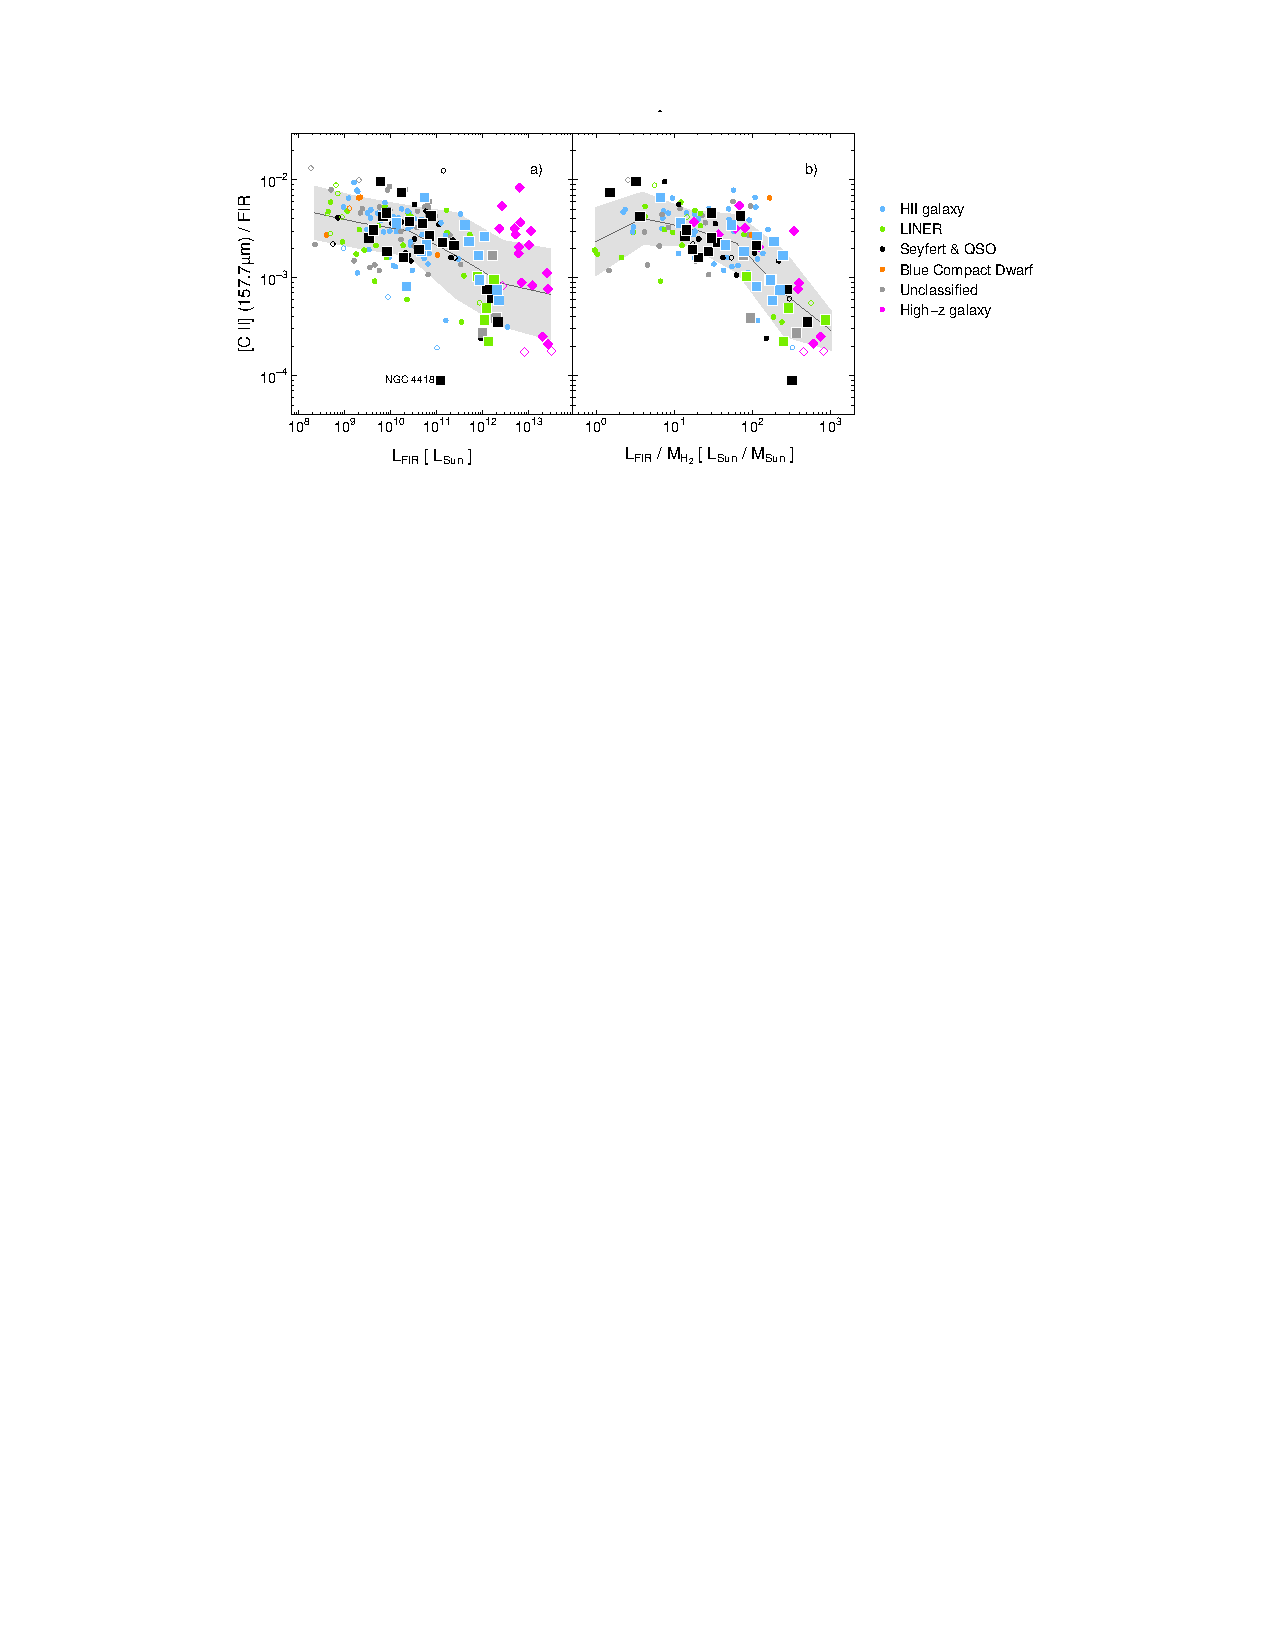
\includegraphics[width=4.5in]{gracia-carpio11_fig1.pdf}
      \end{center}     
    \end{minipage} &
    \begin{minipage}{2in}
      \begin{center}
	\caption{\small {\it Left:} The correlation between \cii\ luminosity
and FIR luminosity for individual galaxies and the $L_{FIR}/M_{H_2}$
relation (as compiled in \citet{gracia-carpio11}.)}
% {\it Right:}
% Expected numbers of detections of galaxies above $5\sigma$ (long
% dashed) and $1\sigma$ (dotted) across the range of redshifts probed by
% \name, based on the number counts of \citet{bethermin12} and the
% observed $L_{[CII]}-L_{FIR}$ relation.}
      \end{center}
    \end{minipage}
  \end{tabular}
 
\label{fig:LCII-LFIR}
\end{figure}

% \begin{figure}[h]
%   \begin{tabular}{ll}
%     \begin{minipage}{3.25in}
%       \begin{center}
% 	\includegraphics[width=3.25in]{sim_blast500.pdf}
%       \end{center}
%     \end{minipage} &
%     \begin{minipage}{3.25in}
%       \begin{center}
% 	\includegraphics[width=3.25in]{sim_channel_map.pdf}
%       \end{center}
%     \end{minipage} \\
%     \begin{minipage}{3.25in}
%       \begin{center}
% 	\includegraphics[width=3.25in]{sim_cii_dist.pdf}
%       \end{center}
%     \end{minipage} &
%     \begin{minipage}{3.25in}
%       \begin{center}
% 	\includegraphics[width=3.25in]{sim_spectrum.pdf}
%       \end{center}
%     \end{minipage}
%   \end{tabular}
%     \caption {\small {\it Upper left:} Continuum image from a
%     simulated \name\ data cube showing the co-addition of spectral
%     channels.  {\it Upper right:} A single spectral channel, showing a
%     detected source.  {\it Bottom left:} Slices of the data cube are
%     amenable to $P(D)$ analysis, as in \Citet{patanchon09} or
%     \citet{glenn10}, to extract the luminosity function of \cii, or
%     the number counts of the continuum.  {\it Bottom right}: A
%     spectrum of the individually detected galaxy. The continuum has
%     been subtracted at each spatial pixel using a 3rd order polynomial.}
% \label{fig:IMapping}
% \end{figure}

\begin{figure}[h]
  \begin{tabular}{ll}
    \begin{minipage}{3.25in}
      \begin{center}
	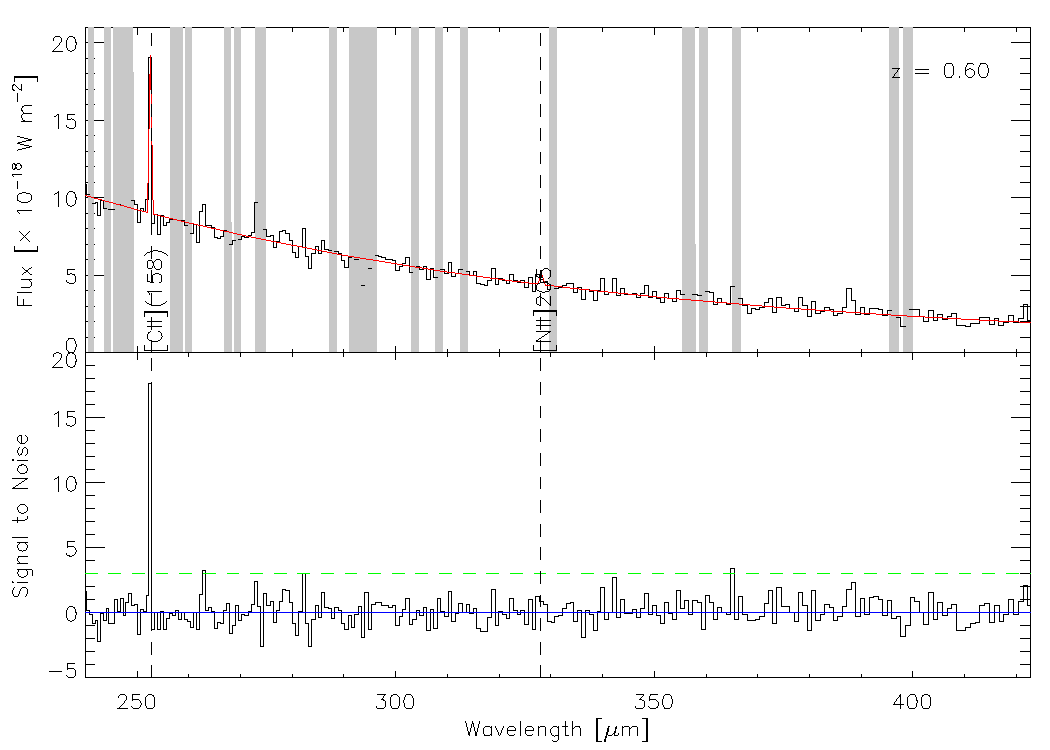
\includegraphics[width=3.25in]{simgal_z060.pdf}
      \end{center}
    \end{minipage} &
    \begin{minipage}{3.25in}
      \begin{center}
	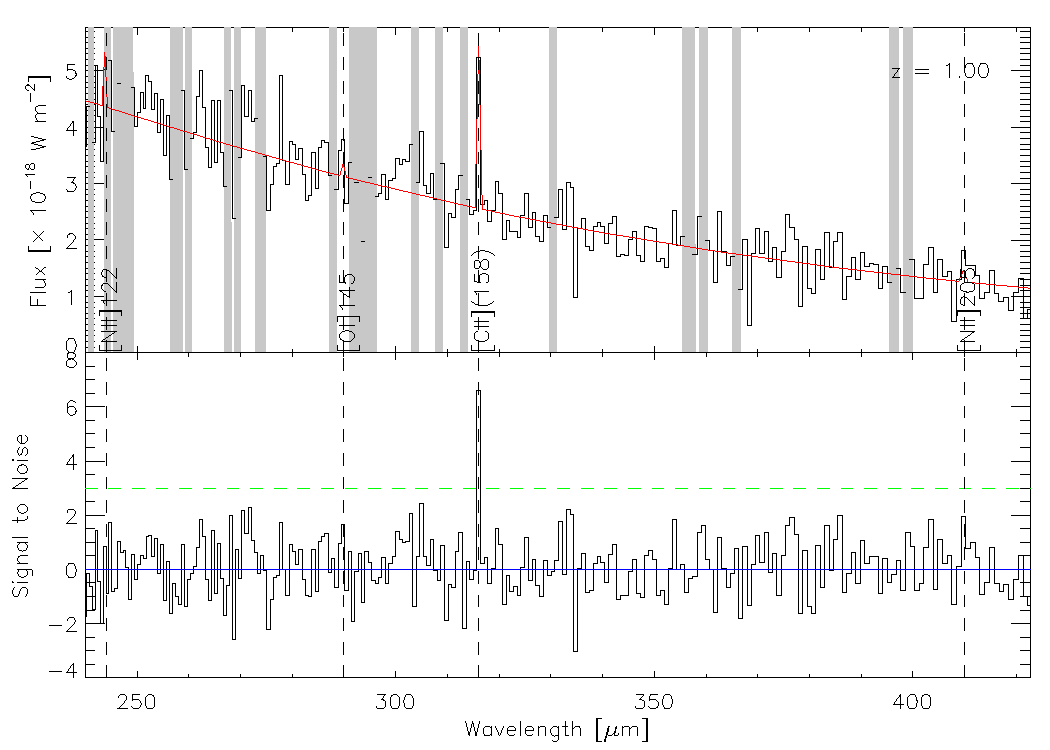
\includegraphics[width=3.25in]{simgal_z100.pdf}
      \end{center}
    \end{minipage} \\
    \begin{minipage}{3.25in}
      \begin{center}
	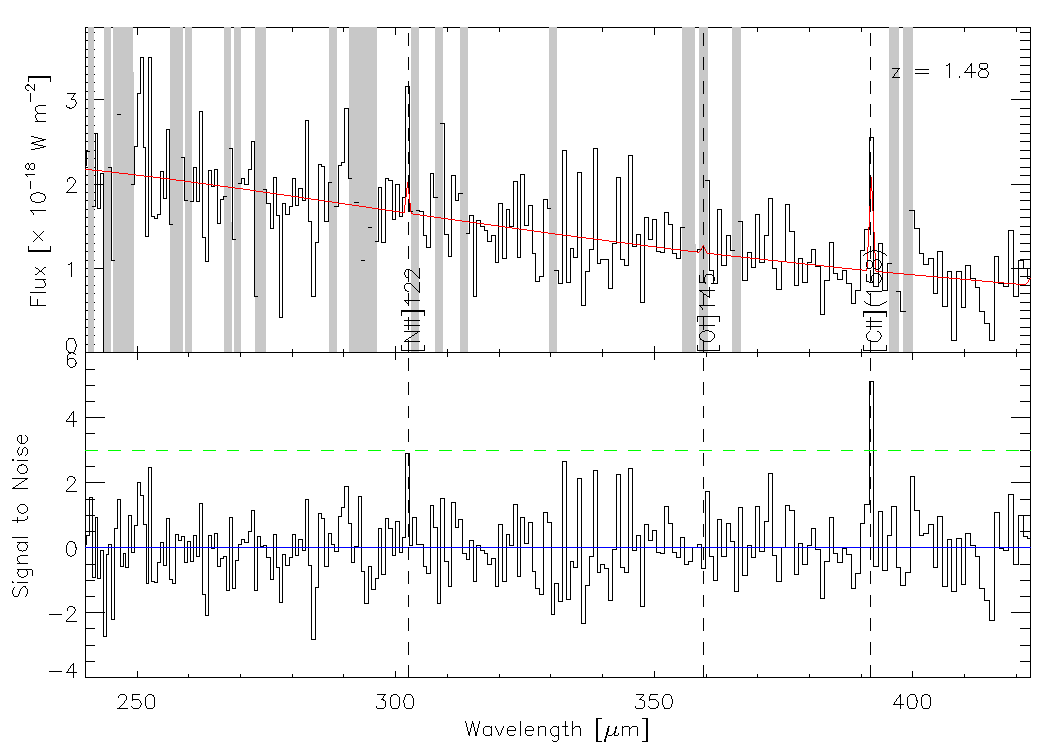
\includegraphics[width=3.25in]{simgal_z148.pdf}
      \end{center}
    \end{minipage} &
    \begin{minipage}{3.25in}
      \begin{center}
	\caption {\small Simulated spectra of galaxies with $L_{FIR}=4\times10^{12}~\Lsun$ at various redshifts for which \cii\ is accessible to \name.  The observations assumed only 10 minutes of integration time.  Note that in addition to the \cii\ line, the continuum is strongly detectect ($T_{dust}=35$~K is assumed), allowing for unambiguous checks on the pointing and calibration.  Channels with $2\times$ higher noise than the median are shown in gray (approximately 11\% of the total), but the lower panel of each figure shows the signal-to-noise accounting for this increased variance, indicating that these channels, while less sensitive, do not create false positives.}
	\label{fig:SimGalaxies}
	\end{center}
    \end{minipage}
  \end{tabular}
    
\label{fig:IMapping}
\end{figure}

\begin{figure}[h]
  \begin{tabular}{ll}
    \begin{minipage}{3.25in}
      \begin{center}
	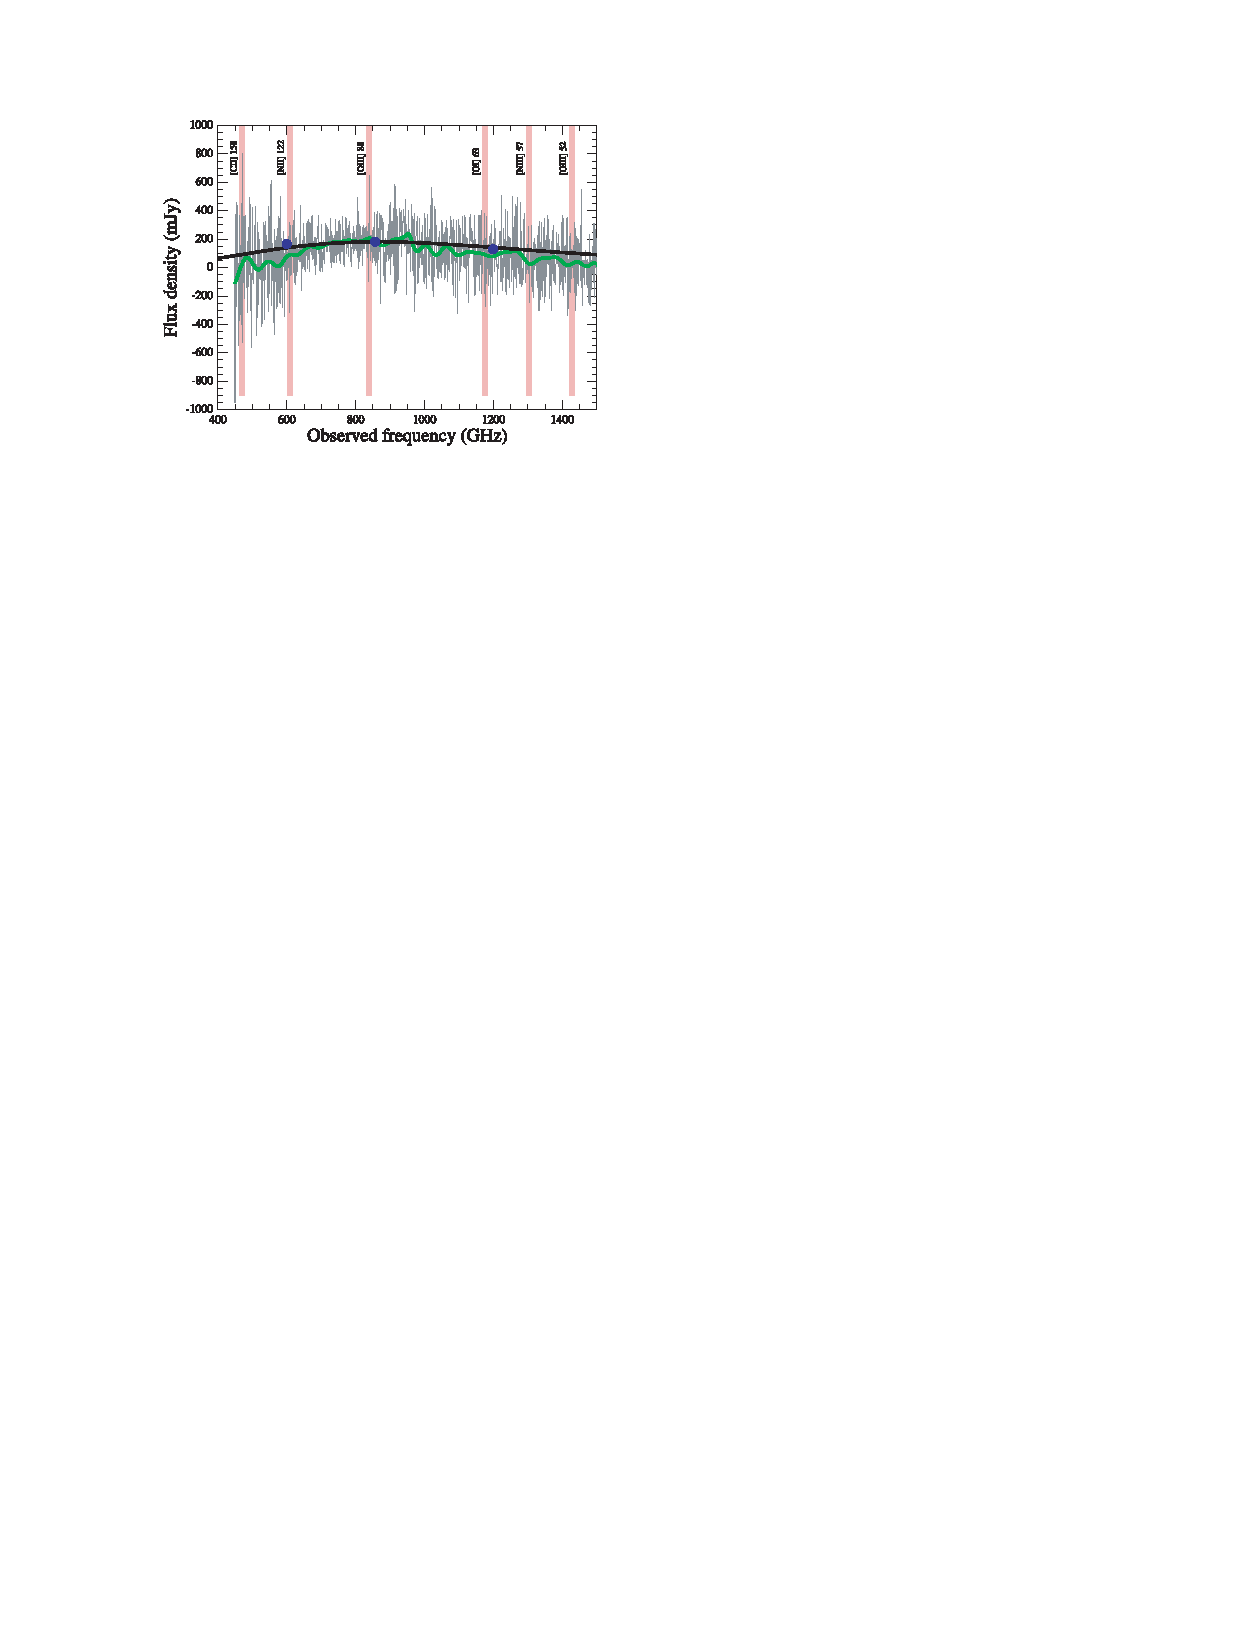
\includegraphics[width=3.25in]{valtchanov11_sdp81_spire_fts_spectrum.pdf}
      \end{center}
    \end{minipage} &
    \begin{minipage}{3.25in}
      \begin{center}
	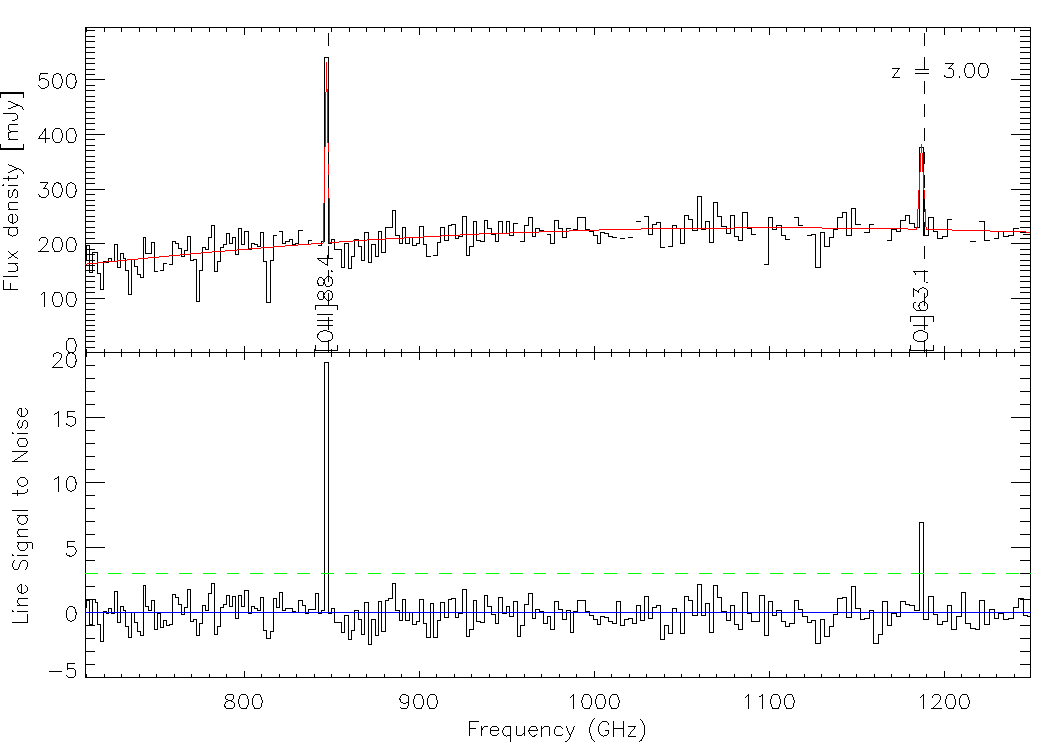
\includegraphics[width=3.25in]{simgal_z300.pdf}
      \end{center}
    \end{minipage} 
  \end{tabular}
    \caption {\small {\it Left:} The \herschel-SPIRE FTS spectrum of SDP.81 from \citet{valtchanov11}, representing nearly 4 hours of integration time.  This galaxy was, at the time of publication, the faintest \cii\ line yet detected by \herschel.  {\it Right:} A similar galaxy observed for 10 minutes with \name.  Though \cii\ has redshifted out of the \name\ band, note the clear detection of \oiii (52 \mum) as well as \oiii (88 \mum).}
\end{figure}

\subsubsection{Power Spectrum of \cii (Science Goal \ref{goal:PowerSpectrum})}

Our overarching goal is to connect the process of star formation in
individual galaxies via their average properties to the properties of
large scale structure (LSS).  To do this requires mapping a large
cosmic volume, and in addition, traditionally requires large
spectroscopic redshift surveys coupled with careful attention to
obtaining photometry for photometric redshifts.  However, in the
far-IR, the process of obtaining redshifts is difficult and slow.
However, the traditional route can be circumvented by {\it intensity
mapping}: making a large data cube in which the third dimension
measured a line, thus providing redshift information.
%\footnote{We note
%that intensity mapping is not a replacement for traditional galaxy
%surveys or detailed studies of individual galaxies, but is rather a
%highly complementary addition to the information gained from them, and
%can profitably be combined with them.  In particular, it provides a
%way of measuring galaxy properties at the clustering scale with small
%error bars and also allows the measurement of the average properties
%of low surface brightness galaxies.}.  
In general, individual galaxies
are not detected, and the information is extracted from the data via a
power spectrum or cross-spectrum.

The most developed case for intensity mapping is that of the 21 cm
experiments attempting to detect the epoch of reionization.\footnote{PI
Aguirre is currently co-PI of NSF AST 1125558 ``Collaborative
Research: Precision Array for Probing the Epoch of Reionization
(PAPER)''.  PAPER is a dedicated attempt to detect the highly
redshifted 21 cm emission from the epoch of reionization.}  At $z \sim
1$, intensity mapping using \hi\ has been proposed for measuring
baryon acoustic oscillations \citep[BAO][]{chang08} and the concept
experimentally demonstrated by the detection of the cross-spectrum of
\hi\ emission with the DEEP2 galaxy survey \citep{chang10}.  Several
theoretical studies have recently been published demonstrating the
feasibility of doing intensity mapping during the epoch of
reionization using CO, \cii\ and other transitions in large-beam
surveys
\citep{carilli11,lidz11,gong11co,gong11cii,visbal11,visbal10}.
% \footnote{We
% also note an experiment described in \citet{zemcov11} similar in
% spirit to intensity mapping, which is attempting to detect the
% signature of the first stars from spectrally-discriminated
% fluctuations in the near-infrared background.}.

With this in mind, we begin by considering the line emission from some
particular species $i$ present in the ISM of galaxies.  (We assume any
continuum contribution has been removed; this is actually
straightforwardly achieved, following schemes which use the spectral
smoothness of the continuum to subtract it.  See, for example,
\citet{bowman09}.)  We have an instrument which acts as an integral
field spectrometer, mapping an intensity data cube
$S(\alpha,\delta,\nu)$, where $(\alpha,\delta)$ are the celestial
coordinates of the line-of-sight along which the spectral frequency
dimension $\nu$ is measured.  Since we are working with line emission,
the observed frequency determines the cosmological redshift and thus
$\nu$ may be transformed into line-of-sight distance, and for each
distance, a transverse dimension may also be obtained.  Thus
$S(\alpha,\delta,\nu) \Leftrightarrow S(\vect{x})$, where $\vect{x}$
denotes comoving spatial coordinates.  The logic of this argument is
laid out for the 21 cm \hi\ fluctuations in, for example,
\citet{morales05}.  We assume that the extent of $\vect{x}$ in the
cube is such that significant cosmological evolution does not occur
over the measured region.

Since the galaxies whose line emission we are measuring trace the
underlying dark matter potential (with some bias), the intensity field
of line emission fluctuations can be written as
\begin{equation}
\Delta S_i(\vect{x}) = \bar{S}_i \bar{b} \delta(\vect{x})
\end{equation}
where $\bar{S}_i$ is average emission line signal, $\bar{b}$ is
luminosity weighted average galaxy bias, and $\delta(\vect{x})$ is the
cosmological overdensity at $\vect{x}$.  In general, since for any
realistic instrument the signal-to-noise at any point $\vect{x}$ will
be low, we will be concerned with the statistical measures on $S$.  In
particular, the power spectrum
% \footnote{Historically, the presence of
% a non-zero-mean instrument noise term (and its corresponding bias) was
% a cause for considerable concern in using the auto-spectrum.  However,
% with multiple measurements of $\Delta S_i(\vect{x})$, it is possible to
% construct auto-spectrum estimators which are unbiased, and thus this
% concern can be removed by proper instrument and observing design
% \citep[e.g., ][]{polenta05,tristram06}.} 
of such a signal is
\begin{equation}
P_i(k) = \bar{S}_i^2 (\bar{b}^2 P(k) + P_s)
\end{equation}
where $P(k)$ is the matter power spectrum, and we have made the usual
assumption of isotropy in the fluctuations.  $P_s$ is a shot (or
Poisson) noise term due to the fluctuations of uncorrelated, discrete
galaxies, from which we have factored the average line brightness.
Note that at the angular scales measured by \name, the clustering
term dominates over the shot noise.  Figure \ref{fig:PowerSpectrum}
shows that a future LDB experiment similar to \name\ with 200 hours of integration would be able to measure the power spectrum of \cii\ emitters with high
signal-to-noise over a range of redshifts and angular scales,
accurately measuring the clustering signal.  With this proposal, we have the sensitivity to detect the highest-$k$ shot noise and set the scale of the \cii\ fluctuations.

% A concern in using the power spectrum of a given line, as has been
% pointed out by \citet{visbal11} and others, is that it may be
% contaminated by foreground line emission from ``interloper lines''
% (lines which share the same observed frequency but not the same
% redshift).  We show the effect of interloper lines for \name\ in
% Figure \ref{fig:AccessibleLines}.  In general, these are expected to
% be fainter than \cii, and at higher redshift.  One way, however, of
% rejecting such interlopers is to use the cross power spectrum of two
% distinct lines
% \begin{equation}
% P_{i,j}(k) = \bar{S_i} \bar{S_j} (\bar{b}^2 P(k) + P_s)
% \end{equation} 
% since interloper lines not at the same redshift will generally be
% uncorrelated in the cross spectrum.  For \name, as shown in Figure
% \ref{fig:AccessibleLines}, the \nii(122), \nii(205), and \oi(145)
% lines are all available for cross-correlation over some portion of the
% redshift range sampled by \cii.  We show that we can detect the
% \cii-\nii\ cross-correlation at $z\sim1$ in Figure
% \ref{fig:NIICrossCorr}.  We will use such a cross-correlation to aid
% in rejecting systematic contamination of the \cii\ power spectra.
% 
% In addition to its role in producing cross-spectra, \nii\ is
% astrophysically interesting in its own right.  It is useful for
% measuring the (unextincted) star-formation rate, and is the basis for
% one of the best measurements in the Galaxy \citep{bennett94}.  The
% 205\mum\ \nii\ line also provides a vital key to the interpretation of
% the \cii\ line.  Because its ionization potential is only 11.3 eV,
% \cii\ may exist in regions of both neutral and ionized hydrogen.
% \nii\ and \cii\ have nearly identical critical densities and second
% ionization potentials (29.6 and 24.4 eV, respectively), so the \nii /
% \cii\ ratio is sensitive only to the relative abundances of the two.
% However, since nitrogen has an ionization potential of 14.5 eV, it is
% present only in ionized hydrogen gas, and thus the ratio
% \cii/\nii(205) probes the fraction of \cii\ present in ionized regions
% \Citep{oberst06}.  This information provides an essential insight into
% the physical origins of the \cii\ emission.
% 
% Flux ratios of emission lines offer a powerful means of extracting
% astrophysics from line emission by constructing quantities in which
% some unknown factor - a physical parameter of the gas - cancels, thus
% allowing the isolation of a particular effect due to the unknown
% physical parameter under investigation
% \citep{osterbrock89,spinoglio92}.  For ionized tracers, different
% lines from the same ion trace {\it density}, as the electron
% temperature is much larger than the relevant energy levels, and the
% abundance drops out. A good example relevant to \name\ is
% \nii(122)/\nii(205). For neutral gas tracers, the gas temperature is
% now no longer necessarily larger than the relevant energy levels, so
% both density and temperature are important. A good example is
% \cii(158)/\oi(145).  The \oi(145) line has a higher critical density
% and upper energy level than \cii, and so the \oi/\cii\ ratio traces
% the combined effects of high densities and temperatures in PDRs
% \citep{malhotra01}.  The cross-spectra of three lines allows the
% construction of two line ratios which are again resistant to
% foreground contamination:
% \begin{equation}
% \frac{P_{l,n}(k)}{P_{m,n}(k)} = \frac{\bar{S}_l}{\bar{S}_m} 
% \equiv R_{l,m}
% \end{equation}
% Using all lines available to us, we will construct these line ratios,
% making detections or constraining their values over a range of
% redshifts.

\begin{figure}[h]
  \begin{tabular}{ll}%{p{3.0in}@{\hspace{0.6in}}p{3.0in}}
    \begin{minipage}{3.25in}% \vspace{-.2in} 
      \begin{center} %\hspace{+0.79in}
	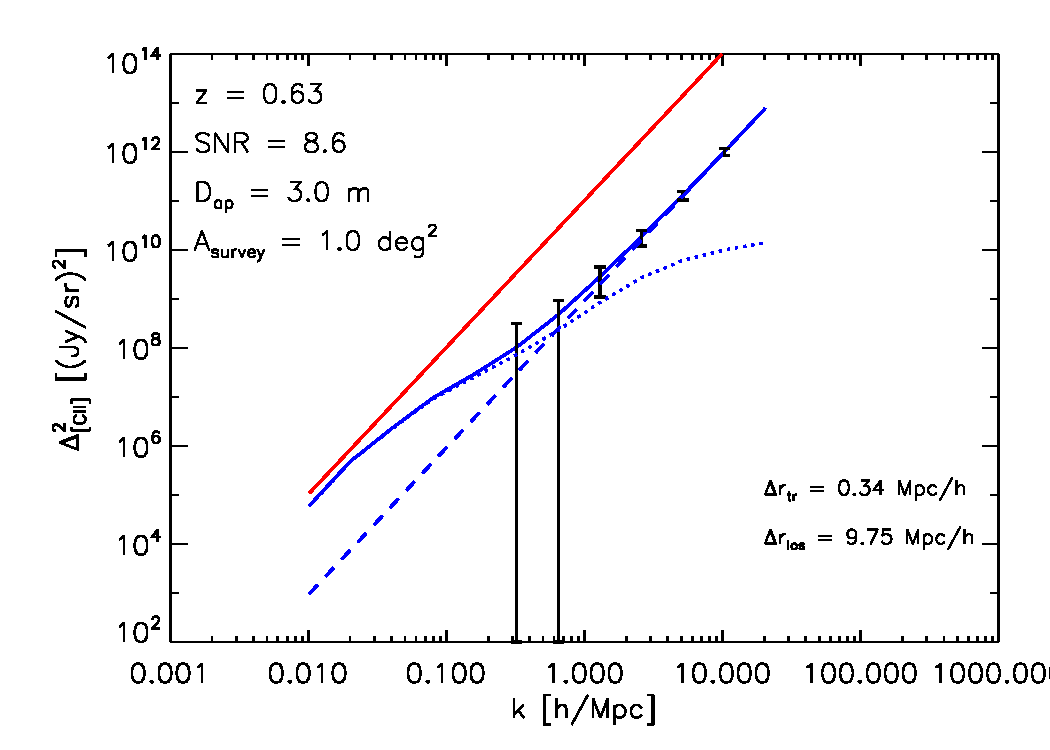
\includegraphics[width=3.25in]{pcii_z63.pdf}
	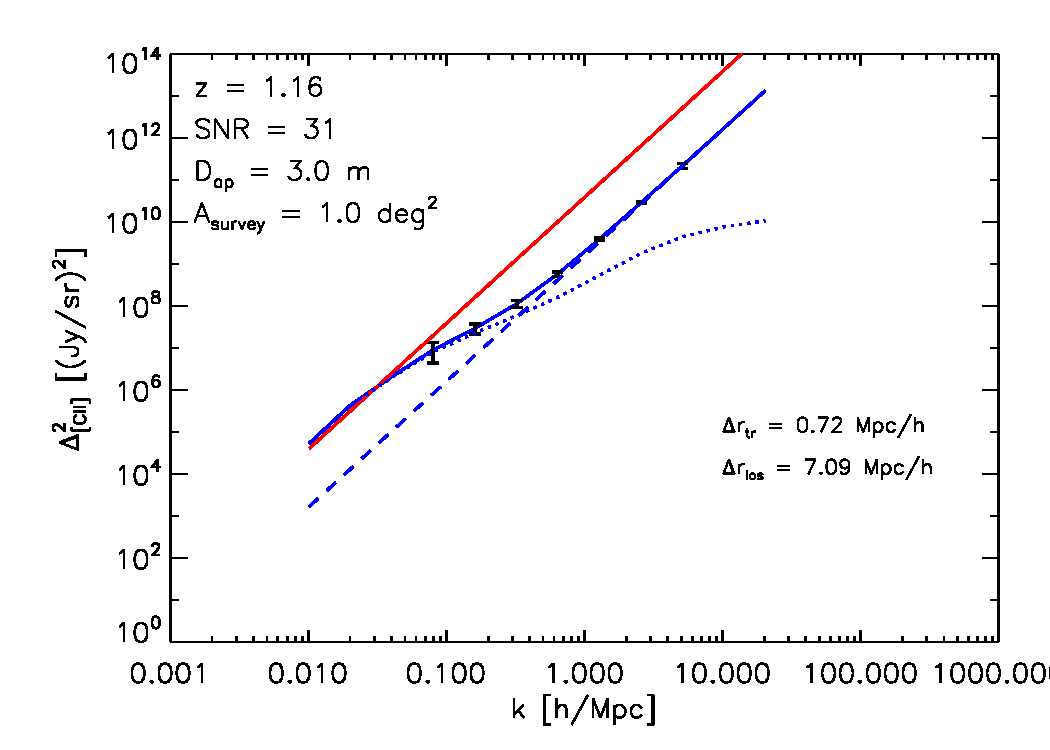
\includegraphics[width=3.25in]{pcii_z116.pdf}
      \end{center}
    \end{minipage} &
    
    \begin{minipage}{3.25in}% \vspace{-.6in}
      \begin{center}% \hspace{+0.79in}
	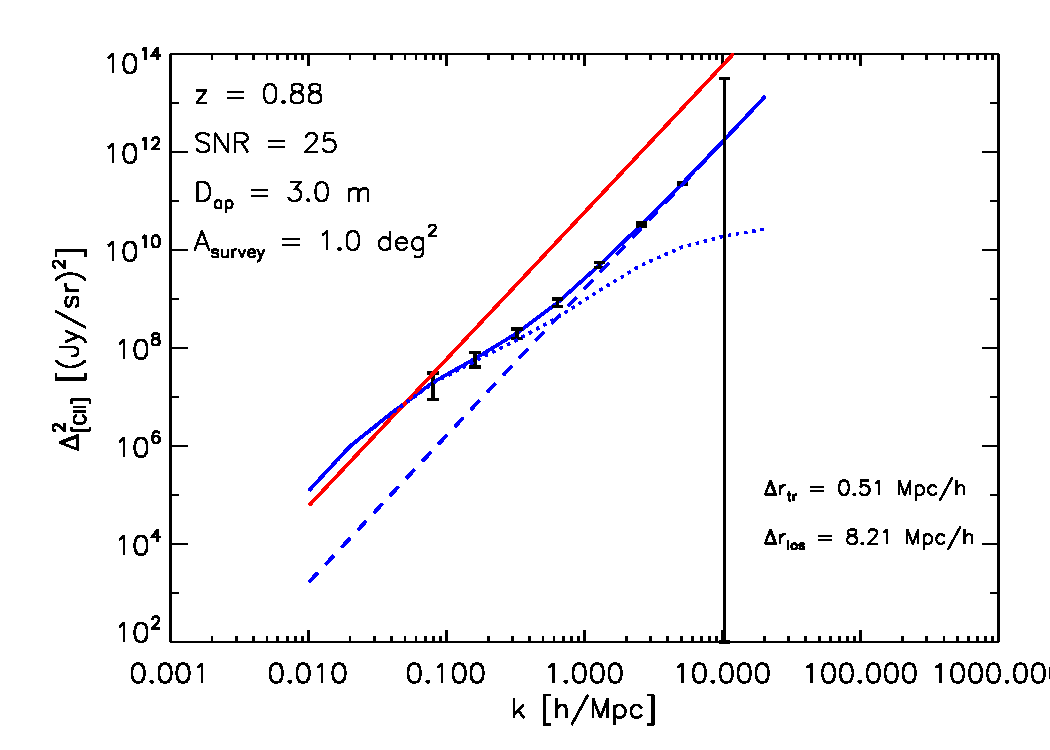
\includegraphics[width=3.25in]{pcii_z88.pdf}
	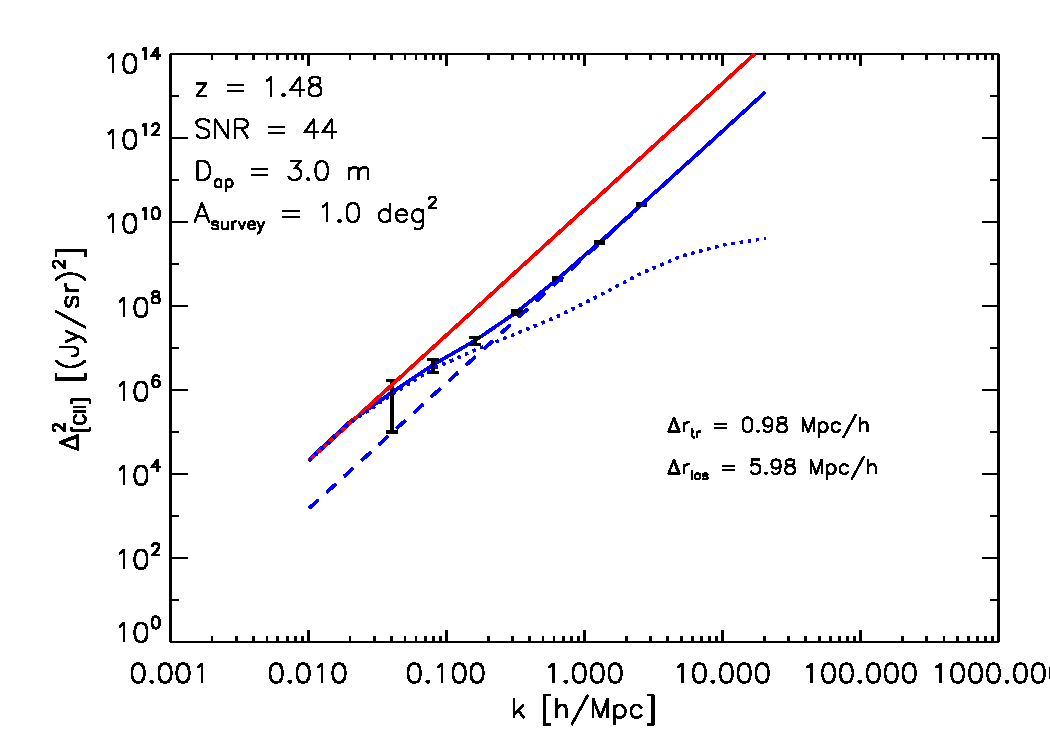
\includegraphics[width=3.25in]{pcii_z148.pdf}
      \end{center}
    \end{minipage}
  \end{tabular}
    \caption {\small Predicted power spectra for the \cii\ line at
    four redshifts.  Dashed lines show the one- and two-halo
    clustering terms, and the dotted line shows ``shot noise'' or
    Poisson term from unclustered galaxies.  Note that the clustering
    raises the amplitude of the power spectrum many orders of
    magnitude above the shot noise expectation.  The vertical black
    dash-dotted lines indicate the range of sales probed by \name,
    i.e., those between $[(2 \pi)^3/V_s]^{1/3}$ and
    $[(2\pi)^3/V_{pix}]^{1/3}$, where $V_s$ and $V_{pix}$ are total
    survey volume and pixel volume respectively.}
\label{fig:PowerSpectrum}
\end{figure}

% \begin{figure}[h]
%   \begin{tabular}{ll}
%     \begin{minipage}{3.25in}
%       \begin{center}
% 	\includegraphics[width=3.25in]{P_CIINII_z1.pdf}
%       \end{center}     
%     \end{minipage} &
%     \begin{minipage}{3.25in}
%       \begin{center}
% 	\caption {\small At $z=1$ both \nii(205~\mum) and
% 	\nii(122~\mum) are available for cross-correlation with \cii\
% 	in the \name\ bands.  Here we show the amplitude of the
% 	cross correlation assuming $b_{CII}=b_{NII}=2.5$, and
% 	$I_{NII}=(0.13+0.05)I_{CII}$, i.e., using a fiducial ratio for
% 	\cii\ to \nii\ emission.  The \nii\ cross-correlation is
% 	particularly important, as it helps to calibrate the relative
% 	fraction of \cii\ emission coming from \hii\ regions versus
% 	those dominated by \hi.}
% 	\label{fig:NIICrossCorr}
%       \end{center}
%     \end{minipage}
%   \end{tabular}
% 
% \end{figure}
% 
% \begin{figure}[h]
%   \begin{tabular}{ll}
%     \begin{minipage}{3in}
%       \begin{center}
% 	\includegraphics[width=3in]{icaris_accessible_lines.pdf}
%       \end{center}     
%     \end{minipage} &
%     \begin{minipage}{3.5in}
%       \begin{center}
% 	\includegraphics[width=3.5in]{line_ratios.pdf}
%       \end{center}
%     \end{minipage}
%   \end{tabular}
% 	\caption {\small {\it Left:} Lines accessible in the \name\
% 	band, as well as potential low- and high-redshift interlopers.
% 	Lines available for cross-correlation with \cii\ at the same
% 	redshift lie between the horizontal black lines.  Interlopers
% 	appearing at the same observed wavelength but different
% 	redshift may be read off along vertical lines.  Interloper
% 	lines at higher redshift than we will map with \cii\ are all
% 	intrinsically fainter than \cii, in addition to their
% 	cosmological dimming.  At lower redshifts, the dominant
% 	contaminants will be high-$J$ lines of CO at redshifts $z<0.5$
% 	Galaxies exhibiting such lines will tend to (U)LIRGs
% 	detectable in the IRAS surveys.  We can also use \herschel\
% 	surveys to identify low-$z$ interlopers. {\it Right:} The
% 	relative strengths of far-IR lines, as observed in M82. \cii\
% 	dominates all lines except \nii(205), with which it will be
% 	cross-correlated.}
% 	\label{fig:AccessibleLines}
% \end{figure}



\section{Instrument}
\label{sec:Instrument}

\subsection{Design Considerations and Sensitivity} 
\label{sec:DesignConsiderations}  

To achieve the scientific and technical goals of \name, we must be able to demonstrate atmosphere-limited performance of the telescope and detectors, and be able to make both pointed observations toward specific objects and small-area maps to validate the sensitivity.  The goal is to detect galaxies with $0.5 < z < 1.5$ in \cii, which sets the wavelength range to 240 - 420 \mum.

The design should be such that the sensitivity of the instrument is
limited by the photon noise of the atmosphere and optics.
%Balloons make attractive platforms for far-IR measurements because of 
%the greatly reduced emissivity and absorption from the atmosphere To 
%take advantage of this, we must design the instrument and optics to 
%have lower noise than the expected atmosphere emission The 
%requirements for a dispersive spectrometer are much more stringent in 
%this regard than for a continuum instrument due to the much smaller 
%bandwidth per detector. 
%The atmosphere will limit the sensitivity in two ways: first, by the 
%background loading, and second by fluctuations in line emission which 
%may mimic a spectroscopic signal Here we only treat the effects of 
%the former; the latter is dealt with by our scanning modulation 
%(Section \ref{sec:Observing}) to remove spatial and temporal 
%fluctuations  
To estimate the atmosphere background, the (proprietary) ATM model of 
Juan Pardo was used.  We have assumed 
%The results for the $T_{RJ}$ of the atmosphere from 50 to 750 \mum\ are shown assuming  
a flight at mid-latitudes, an altitude of 37 km, and 
observations at 45\arcdeg\ elevation.  The ATM model calculates the 
opacity due to all relevant atmospheric species. 
%The antenna temperature is less than 1 K over 75\% (89\%) of the band 
%at 30 (37) km altitude.  
We calculate the noise equivalent power (NEP) due to photon shot noise 
from a greybody with physical temperature $T$ and emissivity 
$\epsilon_\nu$ being detected by a system with optical efficiency 
$\eta$ as 
\begin{eqnarray} 
\label{eq:nep_shot} 
{\rm NEP}_\gamma = \sqrt{\frac{N_{pol}}{2}}2 h \nu \sqrt{n(n+1) \Delta \nu} & , &  
n = \frac{\eta \epsilon_\nu}{\exp{(h \nu / k T)} - 1} 
\end{eqnarray} 
where $n$ is the photon occupation number  
%The two dominant sources 
%of photon shot noise for \name\ are the telescope optics and the 
%atmosphere In order that the photon shot noise limit the instrument 
%performance,  
The detector NEP must be less than the noise NEP$_\gamma$.  
%For
%bolometers, whose noise is dominated by the phonon noise in their
%thermal conductance $G$ to the bath, this is $ {\rm NEP}_{G} = \sqrt{k
%T^2 G} < {\rm NEP}_\gamma$. 
The low noise detectors we will use for
\name\ are discussed in Section \ref{sec:Detectors}. The final figure
of merit for detecting an unresolved line in a point source is given
by the line sensitivity
\begin{equation} 
{\cal S}_\gamma = \frac{2}{N_{pol}}\frac{\sqrt{2} {\rm NEP}_\gamma} 
{\eta_{opt} A_{eff} \rm{e}^{-\tau_\nu}} \; \;
\left[{\rm \frac{W}{m^{2}}~\sqrt{sec}}\right]
\end{equation} 
where $\tau_\nu$ is the atmosphere optical depth, related to the
emissivity as $\epsilon_\nu = 1 - \exp{(-\tau_\nu)}$.  The effective
collecting area, $A_{eff}$, of the telescope is decreased from the
geometrical value $A = \pi (D_{tel}/2)^2$ by
%two factors, the surface 
%efficiency 
%\begin{equation} 
%\eta_{surf} = \exp{(-(4 \pi \sigma_{surf}/ \lambda)^2)} 
%\end{equation} 
%and  
the illumination of the optics.

We have have considered the performance of various potential
architectures for \name, incorporating the atmospheric transmission
and loading, a range of telescope sizes, and the possibility of
actively cooling the telescope to minimize its thermal emission.
While a cooled aperture performs better, it is very costly for a given
aperture size, and the performance improvement is modest because even
a balloon altitudes there is $\sim$1\% emission from the 250~K
atmosphere.  In light of these calculations, and our experience with
ballooning with \blast\ \Citep{devlin04,pascale08} and spectroscopy
with Z-Spec \Citep{inami08,earle06,bradford04,bradford03,naylor03}, we believe we can demonstrate near atmosphere-limited performance using the existing BLAST on-axis \D\ Ritchey-Chr\'{e}tien telescope
%have arrived at a \D\ off-axis 
ambient-temperature telescope, with
carefully controlled primary illumination, Lyot stops at an image of the secondary, and baffling to avoid spillover to warm surfaces.
These parameters and sensitivity factors for our design are given in
Table \ref{tab:Parameters}.

For optimal sensitivity to line emission in distant galaxies, the
spectral resolving power $R \equiv \lambda/\Delta \lambda$ should be
matched to the line width. 
%For \name, we are attempting to achieve a
%balance between sensitivity to invidual objects and to the power
%spectrum; 
For the relatively massive galaxies we are targeting, a resolution $R = 450$ (670 \kms) is adequate: higher resolution increases the number of detectors required and may over-resolve the line.
%in order to ease the requirement on the detector NEP
%(insuring that the system is strongly background limited), and to
%reduce the detector count. 
In principle, the required spectral resolution and large area mapping
could be achieved with either a Fabry-Perot (FP) or FTS spectrometer
design. However, both of these 
%require a moving component, and both
incur sensitivity penalties.
%for follow-up of sources with known
%positions. 
The FP does not cover the entire frequency range instantaneously and
must be scanned, and the FTS places the full optical bandwidth of the
entire band on each detector, increasing the noise. The best approach
is a reflective, blazed diffraction grating, which offers large
instantaneous bandwidth and good sensitivity.
%, with no moving
%parts. 

\subsection{Spectrometer Architecture} 
\label{sec:Spectrometer} 
\Responsible{Hailey-Dunsheath}

%To achieve integral-field spectroscopy over a 2-D field, the spectrometer optics begin by slicing a $5\times5$ pixel field to form a 25 pixel long pseudo-slit, which feeds the spectrometer. 
For optimal efficiency, two independent spectrometer modules and image slicers with separate fields of view are combined to cover the full 240-420 \mum\ range: a short wavelength module covering 240-317 \mum, and a long wavelength module covering 317-420 \mum. 
%The slicing optics follow the same design as successfully implemented in the PACS and
%FIFI-LS spectrometers \citep{looney03apj,looney03spie}; see Figure \ref{fig:Slicer}. 

In Figure \ref{fig:SpectrometerModule} we show the long wavelength spectrometer module. A powered mirror collimates the light passing through the pseudo-slit, and forms an image of the telescope aperture on the grating. The grating itself serves as a cold pupil that controls the telescope illumination. The grating is
operated in first order, and is sized to provide a slit-limited resolving power of $R=450$. A second powered mirror then focuses the dispersed light onto the focal plane. The long wavelength module has a size of $60 \times 32 \times 22$~cm; the linear dimensions of the short wave module are a factor of 1.3 smaller.

The simple spectrometer design employed here produces a moderate amount of
anamorphic magnification, such that the image of a spectrally unresolved
source is stretched in the dispersion direction by 20-50\%. We will use a
hexagonal array of pixels in which the pitch in the dispersion direction
is naturally 15\% larger than in the spatial direction, partially
countering this anamorphism. The final imaging in the long wave module is
at f/2.4, such that an image of a point source is 0.91mm in size. We
design our hexagonal array of microlenses to have a pitch in the spatial
direction of 1.18mm, such that we slightly undersample the spatial
resolution element, and oversample the spectral resolution element. With a
$25\times64$ pixel array we achieve an instantaneous bandwidth of $\approx$$14\%$
for each of the 25 spatial positions, and 2 grating settings (with the
grating tipped by 5.5 degrees) are sufficient to cover the entire
$\approx$$28\%$ band. The short wave module is imaged at f/3.3 to maintain
a constant image size, and the same array of hexagonally packed horns
%microlenses 
will be used to cover this band.
 
Both spectrometer modules are contained within a 1 K optical cavity approximately 70 cm in diameter and 25 cm tall, painted black on the inside and using black baffles to control stray light and keep loading on the detectors low. Light enters this cavity after passing through low pass filters at 77K, 40K, and 4K, with a capacitive mesh bandpass filter at its entrance.  IR blocking
filters between each of the low pass filters cut down on the loading
and increase the cryogen hold time.  The total size of the spectrometer optics will fit with the design for the SuperBLASTpol, as shown in Figure \ref{fig:OpticsInCryostat}.
%leads to a a cryostat of only slightly large overall size and cryogenic volume as the Z-Spec cryostat.

The optical efficiency from the input of the cryostat to the detectors is determined by losses and scattering from a series of optical components.  We tabulate the various components and their various losses in Table \ref{tab:OpticalEfficiency}.

\begin{center}
\begin{tabular}{ll}
Component & Efficiency \\
\hline
Window and 300 K Filter & 0.9 \\
77 K filter & 0.9 \\
4 K filter  & 0.9 \\
Secondary stop & 0.9 \\
Chopping mirror & 0.95 \\
Collimating mirror & 0.95 \\
Grating & 0.7 \\
Focusing mirror & 0.95 \\
Horns and waveguide & 0.8 \\
Detectors & 0.8 \\
\hline
Total & 0.25 
\end{tabular}
\end{center}


% \begin{figure}[t]
%   \begin{tabular}{lc}
%     \begin{minipage}{3.5in}	
% 	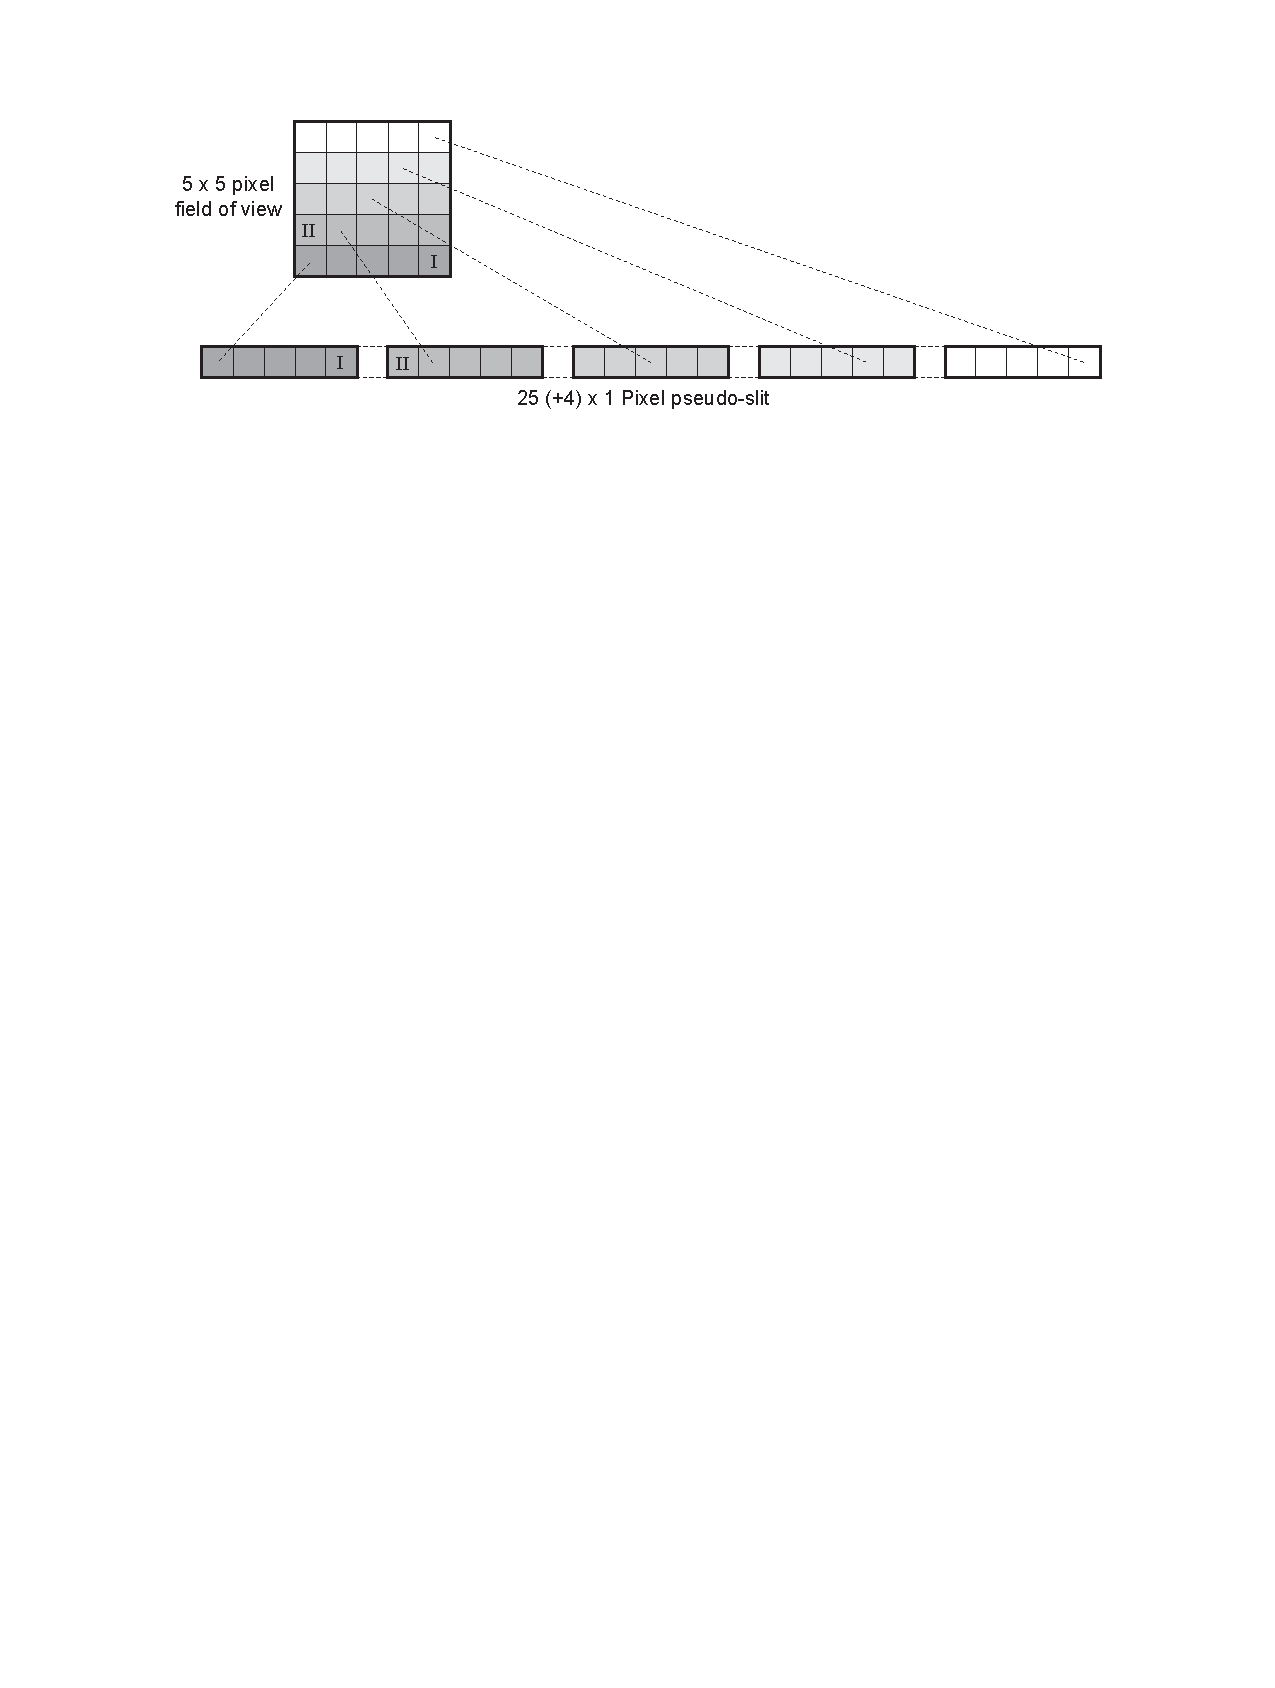
\includegraphics[width=3.5in]{slit_mapping.pdf}
% 	\captionbaseline\caption{\small {\it Right:} The image slicing optics, which present a long pseudo-slit to the spectrometer. {\it Above :} The mapping of the 2-D focal plane to a single long pseudo-slit.  These figures adapated from \citet{looney03apj} for the design of FIFI-LS.}\label{fig:Slicer}
%     \end{minipage} &	
%  \begin{minipage}{3in	}
%       \begin{center}	
% 	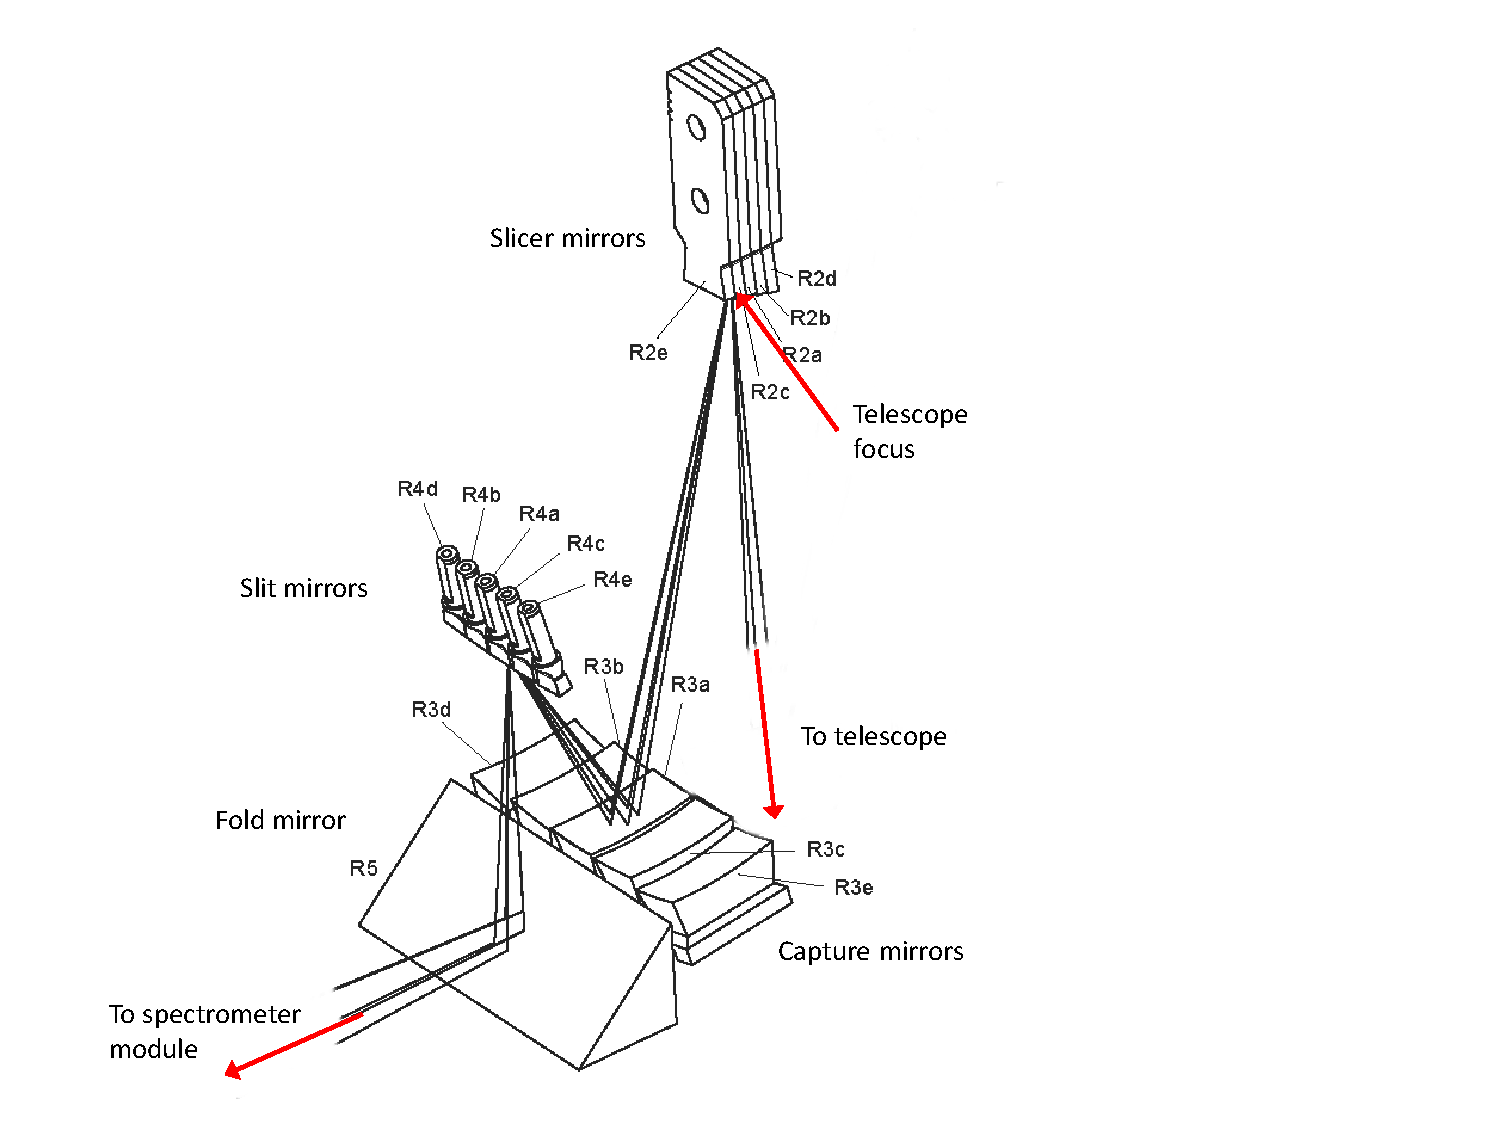
\includegraphics[width=3in]{image_slicer_adapted.pdf}
%      \end{center}	
%    \end{minipage} 
% %   \begin{minipage}{2in}
%  %  \end{minipage}
%   \end{tabular}
% \linefig
% \end{figure}

\begin{figure}[t]
\vspace{0.35in}
  \begin{center}
    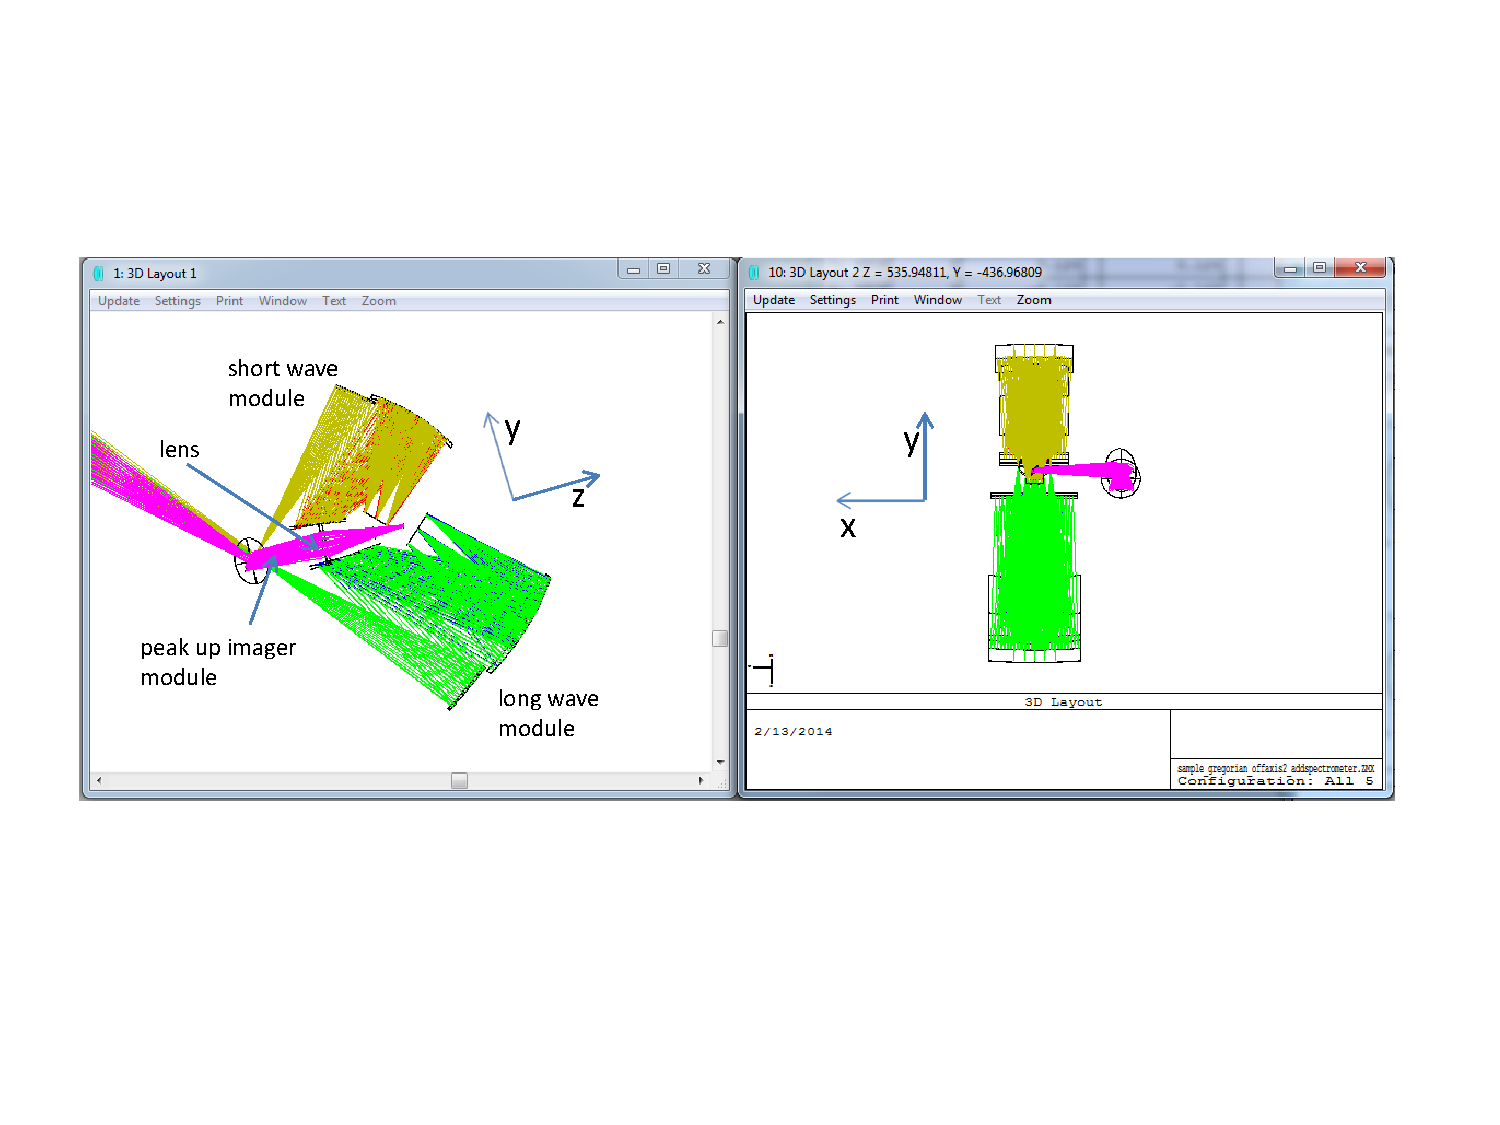
\includegraphics[width=6.5in]{tracking_camera_placeholder.pdf}
    \captionbaseline\caption{\small Ray trace of the optics for the tracking camera and the two spectrometer modules, showing the pick-off of the spectrometer slits from the telescope focus.}
    \linefig\label{fig:TrackingCamera}
  \end{center}
\end{figure}

\begin{figure}[t]
\vspace{0.35in}
  \begin{center}
    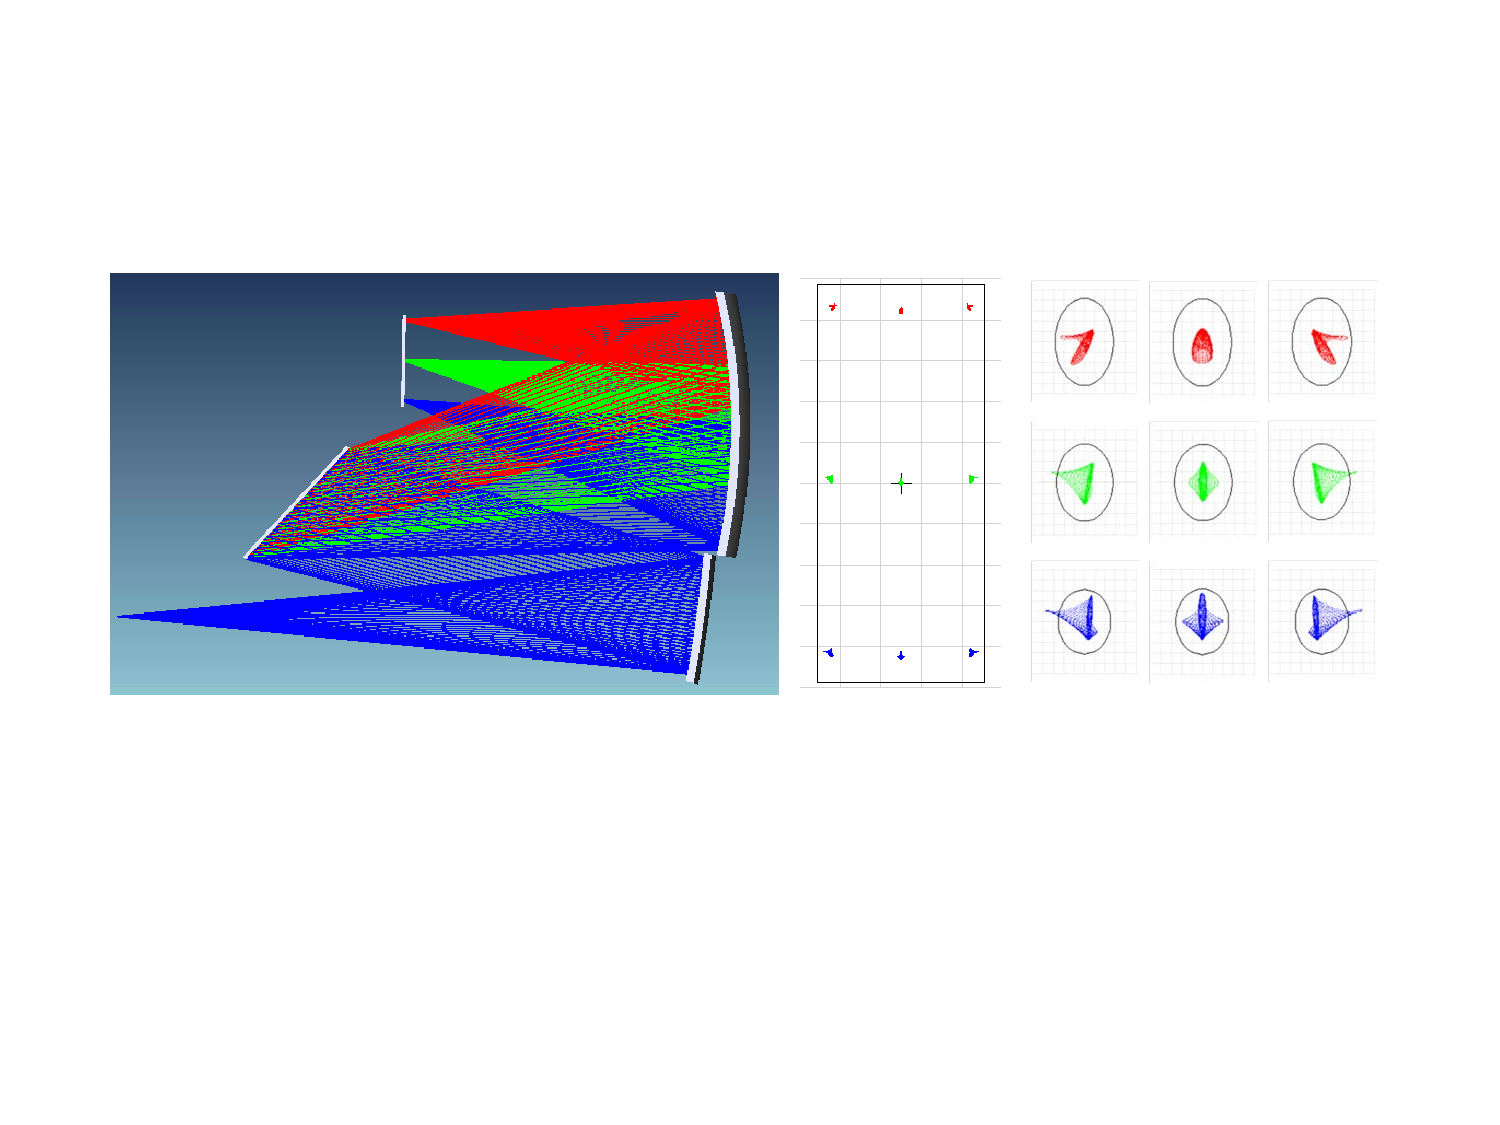
\includegraphics[width=6.5in]{starfire_spectrometer.pdf}
    \captionbaseline\caption{\small {\it Left:} The long wave spectrometer module showing the dispersion and imaging for 3 wavelengths spanning the instantaneous bandwidth. {\it Center:} Image of the array for the 3 wavelengths, and 3 field positions spanning the 25 pixel slit. \R\ Geometric spot sizes for the 9 beams, compared with diffraction-limited Airy disk.}
    \linefig\label{fig:SpectrometerModule}
  \end{center}
\end{figure}

\subsection{Kinetic-Inductance Detector (KID) Arrays}  
\label{sec: Detectors} 
\Responsible{Bradford}

KIDs have emerged in the last decade as a straightforward approach to very large detector arrays for astrophysics.  These devices rely on thin-film, high-Q micro-resonators that absorb incident radiation and respond by changing resonance frequency and line-width.  These changes may be monitored by measuring the complex (amplitude and phase) transmission of an RF or microwave tone tuned to the resonance frequency.  % The response is linear as long as changes in the loading are small.  
Due to the high resonance quality factors (narrow line widths) that can be achieved, large numbers of KIDs may be read out on a single RF/microwave feed line, and the only cryogenic electronics necessary is a single cold (4--20~K) RF/microwave amplifier per transmission line, which may be used for amplifying the signals of thousands of detectors.

KID technology is now approaching the performance levels of the SQUID-multiplexed bolometer systems in ground-based instruments.  One example is the MUSIC camera now at the Caltech Submillimeter Observatory (CSO) \cite{Schlaerth_10} with participation from collaborator J.\ Zmuidzinas, with a total of 2304 detectors in 4 wavelength bands.  Another is the dual-band 150/240~GHz, 224-pixel NIKA camera fielded at the IRAM 30-m telescope by European groups at SRON Utrecht (Baselmans), Institut NEEL (Benoit), and Cardiff (Doyle), which has demonstrated sensitivities approaching the photon background limit  \citep{Monfardini_11, Yates_11,Calvo_13}. 
KID technology has benefitted greatly from the Caltech / JPL discovery of the outstanding properties of titanium nitride (TiN) \cite{LeDuc_10}.   TiN has a high normal state impedance, making it easy to lithograph inductors into direct absorbers.  It has intrinsically high Q values---sQs as high as $3\times10^{7}$ have been achieved with TiN resonators.  These high Qs translate into the ability to build sensitive devices, and NEPs as low as $4\times10^{-19}\,\rm W\,Hz^{-1/2}$ have been measured at Caltech / JPL,  well below the \name\ requirement of NEP$_{\rm BG}\sim2\times10^{-18}\,\rm W\,Hz^{-1/2}$.   A final key feature of TiN is the ability to tune the \Tc\ over a range from 0.8 to 4~K by varying film deposition conditions to tailor the response to a given application.  

\vspace{0.05in}{\bf Measured TIN KID Q and responsivity.}   With these excellent properties demonstrated, TiN in lumped-element KIDs have become the focus of the Caltech / JPL effort, and our group has demonstrated the key properties of TiN KIDs through the 350-\mum\ MAKO camera development.  
First, we have shown that KIDs using TiN inductors provide Qs of 10$^5$ when operated at a base temperature of \Tc /5, this sufficiently suppresses thermal quasiparticle excitations. 
Next, we have carefully measured the response of the TiN with the MAKO prototype arrays.  The response of a given KID (\response) is expressed as fractional frequency shift per input power ($\delta$f/f per W).  However, the response is really due to changing the quasiparticle density in the inductor, so that with a given material and readout frequency, a KID system can be  characterized by a fractional frequency response to {\it power density}: $\mathcal{R}_V = \mathcal{R}_x\!\times\!V$ with units of ($\delta$f/f)/(W\mum$^{-3}$). This volume-response product is the key materials parameter for specifying KIDs for lower-loading applications.  KID responsivity can be increased  by simply reducing the inductor volume.

\vspace{0.05in}{\bf KID sensitivity and two-level system (TLS) noise.}  
The  sensitivity of a KID is expressed as a ratio $\mathrm{NEP = \sqrt{\mathrm{S_{xx}}}/\mathcal{R}_X}$, where \response = $\mathcal{R}_V / V$ is the response, as described above.  \Sxx\ is the variance in the fractional frequency fluctuations $\mathrm{(\delta f/f)^2\,Hz^{-1}}$.  The mechanism giving rise to \Sxx\ in KIDs has been the subject of intense study by our group, and is now known to arise from fluctuations of the resonator capacitance due to the presence of
microscopic two-level-system (TLS) fluctuators in amorphous
dielectrics \cite{Gao_07,Kumar_08,Gao_08a,Gao_08b,Noroozian_09}.
The noise does \textit{not} arise in the kinetic inductance
detecting element itself, so it is possible to engineer the device to bring the TLS noise well below the
fundamental photon noise.    For \name, as with MAKO and all of the current generation of KID systems, the first step is to bring the readout frequencies
down from the microwave range (few GHz) into the RF range ($\sim\rm few\,\, 100$ MHz)
%because \Sxx\ due to TLS fluctuations has a 1/$f_{\rm readout}^2$ dependence 
to achieve high $Q$ (good muxing) with small volume (high responsivity) and to use cheaper, simpler electronics (see \cite{Zmuidzinas_12} for details).  Another key parameter is the capacitor electrode spacing $g$, or pitch of the interdigitated capacitors: increasing the pitch reduces the electric field in the dielectric, reducing the noise according to \Sxx$\propto g^{-1.6}$.   Finally, we have developed a new pixel array architecture particularly well-suited to \name\ and the other low-background applications in which all amorphous dielectric layers are eliminated.  It consists of simply a single layer of TiN patterned on the crystalline silicon wafer (Figure~\ref{fig:makonew}).   As Figure~\ref{fig:makonew} shows, \Sxx\ in this device is $1.0\times10^{-18}\,\rm Hz^{-1}$, a factor of 5--10 lower than the previous generation of devices using 2--3 metal layers and amorphous dielectric films.  The MAKO prototype 350\mum\ arrays are demonstrating in detail these sensitivity improvement; they are now clearly 
showing photon-noise-limited performance in laboratory measurements with 95\% pixel yield.   

\begin{figure}[t!]
\begin{center}
\includegraphics*[height=7.25cm,trim= 2cm 0cm 1cm 2cm]{mako_newarray}
\includegraphics*[height=7.25cm,trim=1cm 0.2cm 1cm 0.5cm]{icaris_nep}
%\includegraphics*[height=4.3cm,trim= 14cm 12cm 20cm 16cm]{mako_newarray}
\includegraphics*[height=7cm,trim= 9cm 5.5cm 16cm 8.2cm]{mako_new_ledit}\\
%\includegraphics*[width=8cm,bb=10 80 600 450]{MAKO_1}
%\vspace{-0.2in}
\captionbaseline\caption{\small  \name\ lens-coupled TiN KID array architecture.   Top, left shows a 432-pixel KID array (die is 22.5~mm on a side) for the MAKO 350-\mum\ ground-based camera.  A similar array has demonstrated photon-noise limited performance in the lab and is en-route to the CSO as of this writing.  Bottom shows the pixel detail.  A single TiN layer forms the both the meandered inductors (circular features) and the interdigitated capacitors (rectangular features).  The thick horizontal traces are the feed lines traversing the array (alternating polarity, so every other feedline is an effective ground).  This pictured device has hexagonal packing (shown schematically in black) with a per-pixel area of 1~mm$^2$ (1.07~mm short hex spacing), and is tuned for MAKO loading.  \name\ will use a similar design with a slightly larger total pixel area (1.36~mm short hex spacing) but smaller circular inductor (200~\mum\ diameter instead of the pictured 350~\mum\ diameter).  Top, right shows the 
fractional frequency noise measured in this device at 200~mK (left axis).  The right-hand axis shows the inferred NEP which will be obtained with the inductor specified for \name.  The rolloff above 200~Hz shows the resonator bandwidth, ample for \name. The rise below 1 Hz is due to a thermal drift in the stage temperature---it is unique to this measurement, and common across the array, so not relevant for \name. }
\linefig\vspace{-0.35in} \label{fig:makonew}
\end{center}
\end{figure}

\vspace{0.05in}{\bf Pixel design for \name.} \name\ will use this single-layer architecture, and the same 100--250~MHz resonant frequencies as MAKO.  It requires straightforward adjustments to accommodate the low loading and meet the required NEP.  First, we will reduce the volume of the meandered inductor by a factor of 16, increasing its response by this same factor.  The requirement to impedance match to the incident wave results in a invariant scaling between volume and area (a constant effective thickness), so that the volume reduction is also the area reduction.  The \name\ KID inductors will be patterned into circles of diameter 200~\mum.  Coupling through a microlens array (described below) will preserve good focal-plane filling.  The smaller inductor can provide the same total inductance, by simply meandering a smaller-width trace than (1.0~\mum\ wide instead of 2~\mum) -- our experience indicates that the failure rate is due to the total number of squares in the inductor, which is invariant 
since it scales as L, so we anticipate high yield ($>$90\%) as obtained with MAKO.  Second, we will use a lower \Tc\ TiN film, targeting 0.9~K instead of the 1.3~K used in MAKO.   Since the response scales at least as \Tc$^{-2}$, this provide a further factor of 2.1 increased response.  \Tc$\sim$0.9~K requires operation at T$\sim$180~mK, scaling from MAKO, but we baseline 150~mK to carry margin.  This is readily achievable with high duty cycle with a commercial adiabatic demagnetization refrigerator (ADR).   

To offset the increase in TLS noise due to the lower operating temperature, we will increase the electrode spacing $g$.  NEP$_{\rm TLS} \propto \sqrt{\rm S_{\rm XX}} \propto \rm T_{\rm op} / g^{0.8}$, so a factor of 1.4 increase in $g$ is required to recover the measured TLS noise measured at 200~mK (Figure~\ref{fig:makonew}).   The larger $g$ reduces the capacitance slightly, but it can be compensated with an comparable increase in area, possible with our larger pixel pitch relative to the MAKO prototype.  In any case, the impact on the KID resonant frequency is small ($f=1/\sqrt{LC}$), and the devices will still lie in our target readout band extending up to 250~MHz.

\name\ will field 2 arrays, each with 64 (spectral) $\times$25 (spatial) =1600 detectors, packed hexagonally with a 1.36-mm pitch.  Each will require 2 readout chains, with $\sim$800 channels each.  The goal will be to field this on a single wafer-sized die, but mosaicing 2 dies into the package is a fallback option, producing only a small gap in the spectral direction which can moved away from lines of interest by tuning the grating.  The package will provide a free-space $\lambda/4$ backshort under the device wafer, as used in MAKO.

\vspace{0.05in}{\bf Horn array.}  {\bf \color{red} TBD}
% Concentrating the radiation onto the small inductor requires a concentrating lens, and lens arrays have been designed and prototyped by our group.   Figure~\ref{fig:lenses} shows a prototype silicon lens array machined by Veldlaser (Heerenberg, Holland), as well as the measured profiles.   While \icaris\ requires somewhat greater concentration than these lenses, corresponding to a faster lens with greater curvature, this is not a problem for the laser manufacturing processes as arbitrary depths are possible.  We have performed electromagnetic simulations to verify that good efficiency can be achieved coupling to the 200-\mum-diameter. (Figure~\ref{fig:lenses}).   The lens is a hyperboloid with a total sag of 300~\mum (if sized at 1.5 mm), and it provides a total efficiency of $>$75\%.  To provide an anti-reflection (AR) coating, the lenses will be coated with a quarter-wavelength layer of parylene, a standard electronics packaging process.  The microlens arrays will be simply clamped to the KID arrays, aligned using a pin and slot jig.

\begin{figure}[t!]
\begin{center}
\captionbaseline\caption{\small {\bf \color{red} THIS FIGURE TO BE REPLACED WITH HORN ARRAY.}}  
%Microlens arrays. TOP: 1-mm pitch lens array prototype machined from a silicon wafer by Veldlaser, with measured profile over several lenses shown at right.  BOTTOM:  f/0.8 microlens design for ICarIS, with hexagonal packing.  This simulation is for a 1.5-mm diameter lens as an upper bound to the final lens size, in order demonstrate sufficient power concentration.  HFSS simulations indicate 75\% of the power incident in a uniform plane wave is coupled to the designed 200-\mum\ diameter inductor.  The coupling to a more centrally-concentrated field distribution (such as the image of a point source centered on the pixel) will be higher. }
\linefig\vspace{-0.35in} \label{fig:lenses}
\end{center}
\end{figure}


\subsection{Readouts}
\label{sec:Readouts}

In order to achieve frequency domain multiplexing of KID arrays, two tasks must be accomplished: 1) A waveform consisting of a sum of frequency tones (each at an individual pixel frequency) must be generated and transmitted to the array and 2) after interacting with the pixels, the complex transmission of the individual tones must be extracted from the waveform.  The first task is easily accomplished using a cyclic memory buffer and a DAC to continuously play back a pre-calculated periodic waveform.  The second task can be accomplished using advanced digital-signal processing hardware.  A fast, large-dynamic-range ADC is followed by a Field Programmable Gate Array (FPGA) which performs frequency separation utilizing a fast Fourier transform or more sophisticated techniques.  

\name\ will use a multiplexing readout system developed by the Caltech / JPL group for 100--250~MHz KID arrays.  This readout leverages the Reconfigurable Open Architecture Computing Hardware (ROACH) platform developed by the Berkeley CASPER group which features a Xilnix Virtex-5 FPGA.  An additional daughter card provides two 1 GSPS DACs and two 500 MSPS ADCs.  500 MB of memory on the ROACH enables waveform playback by both DACs simultaneously.  The readout uses custom FPGA firmware developed specifically for KID readout.  The firmware implements a polyphase filter bank (PFB) to achieve an initial stage of coarse frequency separation.  This is followed by multiplication of the PFB channels by pre-specified sinusoids and then low-pass filtering.  This second stage allows fine-frequency separation of the waveform while avoiding calculation at frequencies containing no pixel information, resulting in a substantial savings of FPGA resources.  This readout is working in the laboratory and is being deployed with 
the MAKO 350-\mum\ camera at the CSO telescope as of this writing.  For the MAKO pixels, as will be the case for \name, the total noise from the cold amplifier and readout electronics is a comfortable factor of 3 lower (in \Sxx\ units) than the noise from the devices themselves.   A single readout is capable of performing simultaneous complex transmission measurements of $>2000$ tones at a rate of 25 Hz, plenty of margin on the 800 detectors per readout chain we intend to use with \name.
%For this first field demonstration, a single ADC/DAC pair is being used to readout the 432 pixel MAKO array.  The FPGA firmware is expected to be upgraded in the near future to support both ADC/DAC pairs allowing two arrays to be readout simultaneously with a single ROACH.  

Proper power budgeting requires understanding readout power consumption.  A single roach board draws 86 W of power.  Additionally, a readout computer 
%requiring $\sim$100 W of power 
is used to perform post-processing of the data and storage of the time stream.  Conservatively, a single computer can service two ROACH systems.  We can use computers optimized for lower power consumption  For 4 ROACH systems, we therefore estimate a power consumption of less than 500 W, a manageable figure, particularly for the short flights we envision.  

\subsection{Telescope}
\label{sec:Telescope}

The telescope design must be lightweight and compact, with low overall
emissivity and high-efficiency coupling to the spectrometer.  To
reduce the emissivity, we have gone with an off-axis design which is
nevertheless fairly compact and rigid.  This led to an off-axis
Gregorian design, with a parabolic primary with \D\ of projected
aperture and an elliptical secondary.  The secondary focus is located
$\sim50$ cm behind the surface of the primary to allow plenty of room for
backing structure, cryostat windows and filters.  The maximum field of
view (defined as when the beam at 300 \mum\ drops to a Strehl ratio of
0.95) is 0.5\arcdeg\ in diameter.  This is much larger than required
for \name, and could be reused for other imaging submillimeter
balloon missions.

The primary mirror will be machined of aluminum, similar to the mirror
built for BLAST.  The 1.8 meter BLAST mirror was re-made in 2009 by
Magna Machining in Ohio.  A diamond tool was used to machine the
surface to an RMS of 0.45 microns with a form error less than 3.5
microns.  We recently had this verified at L3-Brashear in Pittsburgh,
PA.  The larger primary proposed here will require further
investigation to ensure it can be manufactured, but the technology is
very similar to BLAST and ACT.

The secondary will be diamond turned by OASYS Technology (formerly
Diamond Turning Inc.), the same company that machined the BLAST
secondary mirror.  By virtue of the off-axis design, the secondary
support structure does not produce additional load on the detectors.
However, the size and weight of the secondary has fundamental impact
on the reliability of the pointing due to gravitational deflection of
the secondary support.  We have specified a very rigid support
structure (see Figure \ref{fig:Gondola}, and will lightweight the
secondary as much as possible.

Because of the different materials used for the mirrors and supports
(aluminum and carbon fiber), the difference in the coefficient of
thermal expansions would cause the telescope to go out of focus with
changes in temperature.  We will use the BLAST focusing system which
has three precision actuators behind the secondary to provide 3 micron
positioning (Figure~\ref{fig:SecondaryPositioning}).  The entire
system worked flawlessly during the BLAST 2006 flight.

In our sensitivity calculations and the parameters in
Table~\ref{tab:Parameters}, we have assumed that the temperature of
the mirror is 250 K, the ambient air temperature at balloon float
altitudes.  Based on previous balloon missions (e.g.,
\Citet{2005ApJS..160...59S}), with sufficient high reflectivity
baffling around the telescope, it can passively radiatively cool to
200 - 220 K, improving our sensitivity slightly.  We also assume a
93\% illumination for the primary.

\begin{figure}[t]
 \begin{tabular}{ll}
   \begin{minipage}{3.0in} \vspace{-.2in} 
     \begin{center} \hspace{+0.79in}
       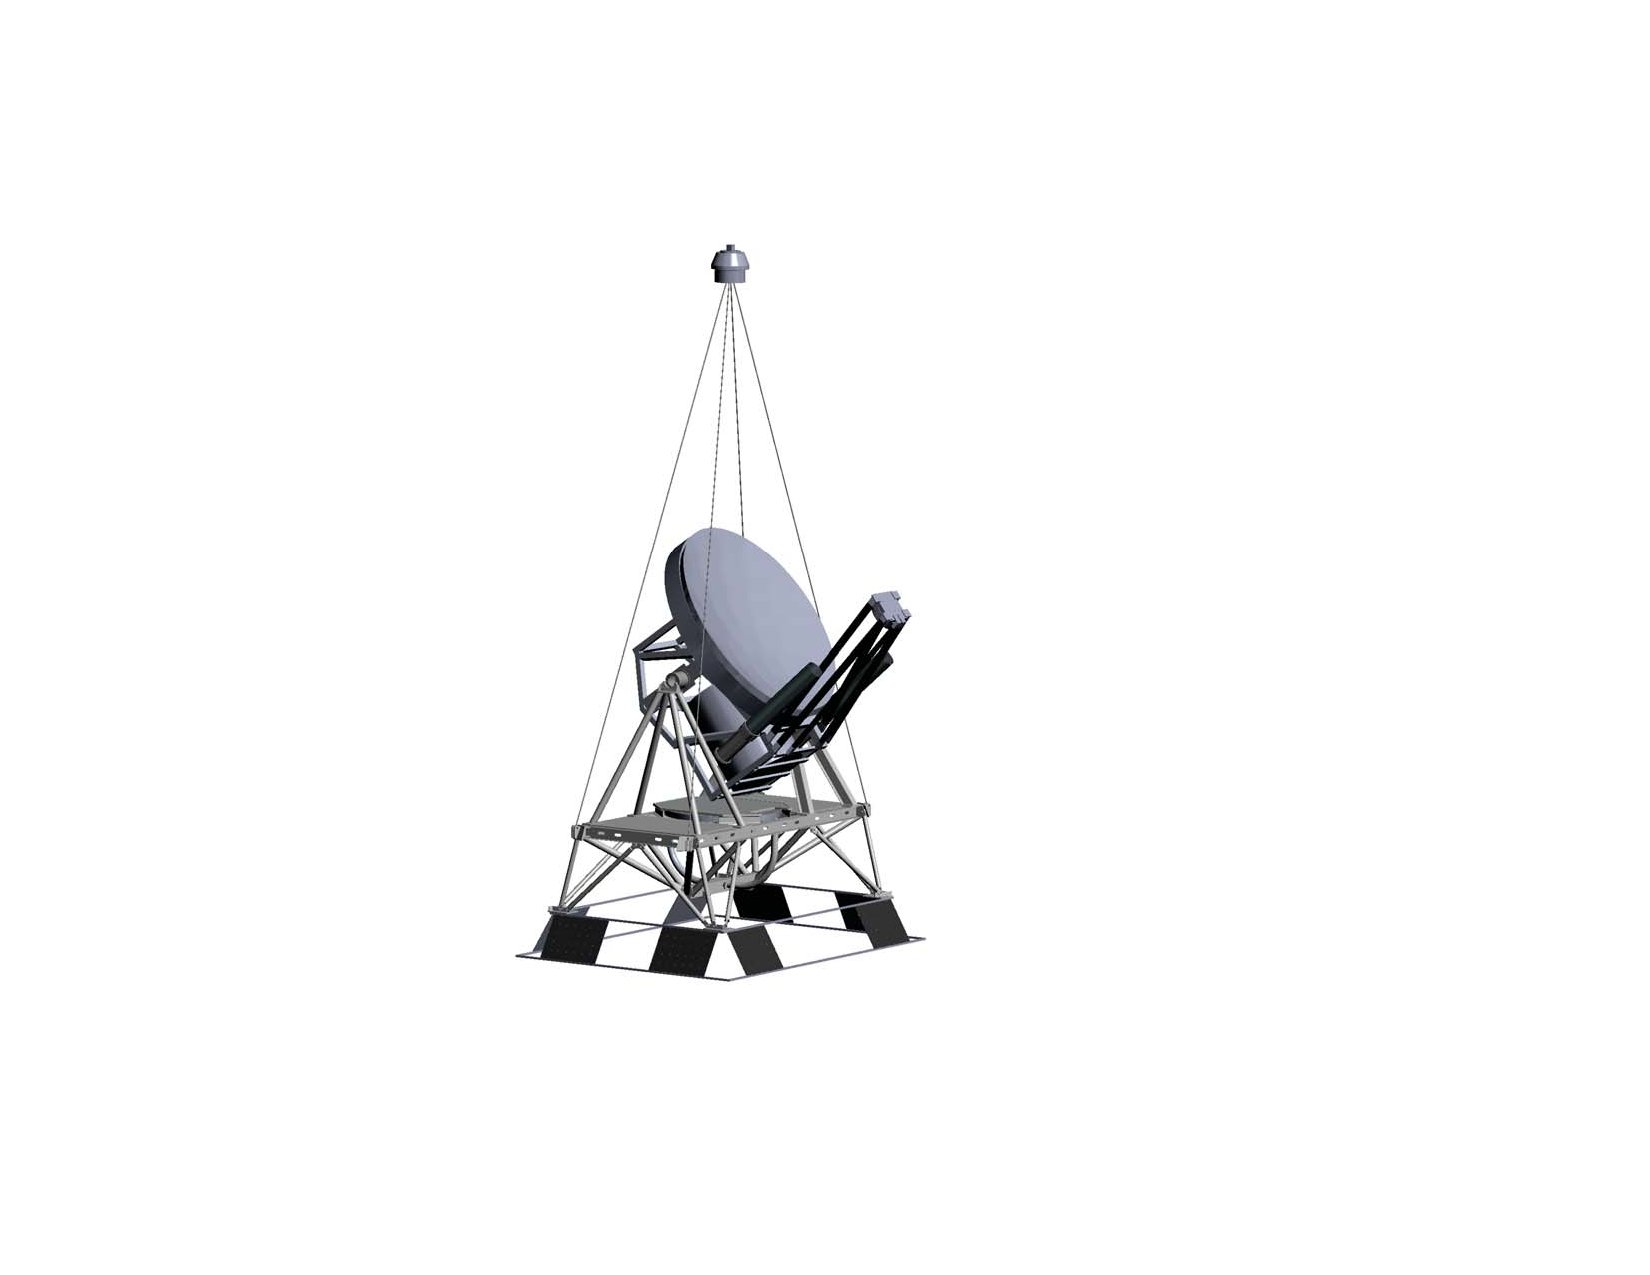
\includegraphics[height=4.5in]{ICarIS_gondola.pdf}
     \end{center}
   \end{minipage} &
   \begin{minipage}{3.5in} \vspace{-.2in}
     \begin{center} \hspace{+0.79in}
      \captionbaseline\caption{\small A Solidworks rendering of the \name\ telescope
showing the off-axis optical design and the approximate size and
location of the cryostat and star cameras.  The Sun shields are not
shown.  The structure is based on the proven \blast\ design.  The
frame will be made from carbon fiber and aluminum.  The upper part of
the gondola supporting the primary has been redesigned slightly from
the \blast\ architechture to support the larger off-axis \D\ mirror.}
       \label{fig:Gondola} 
       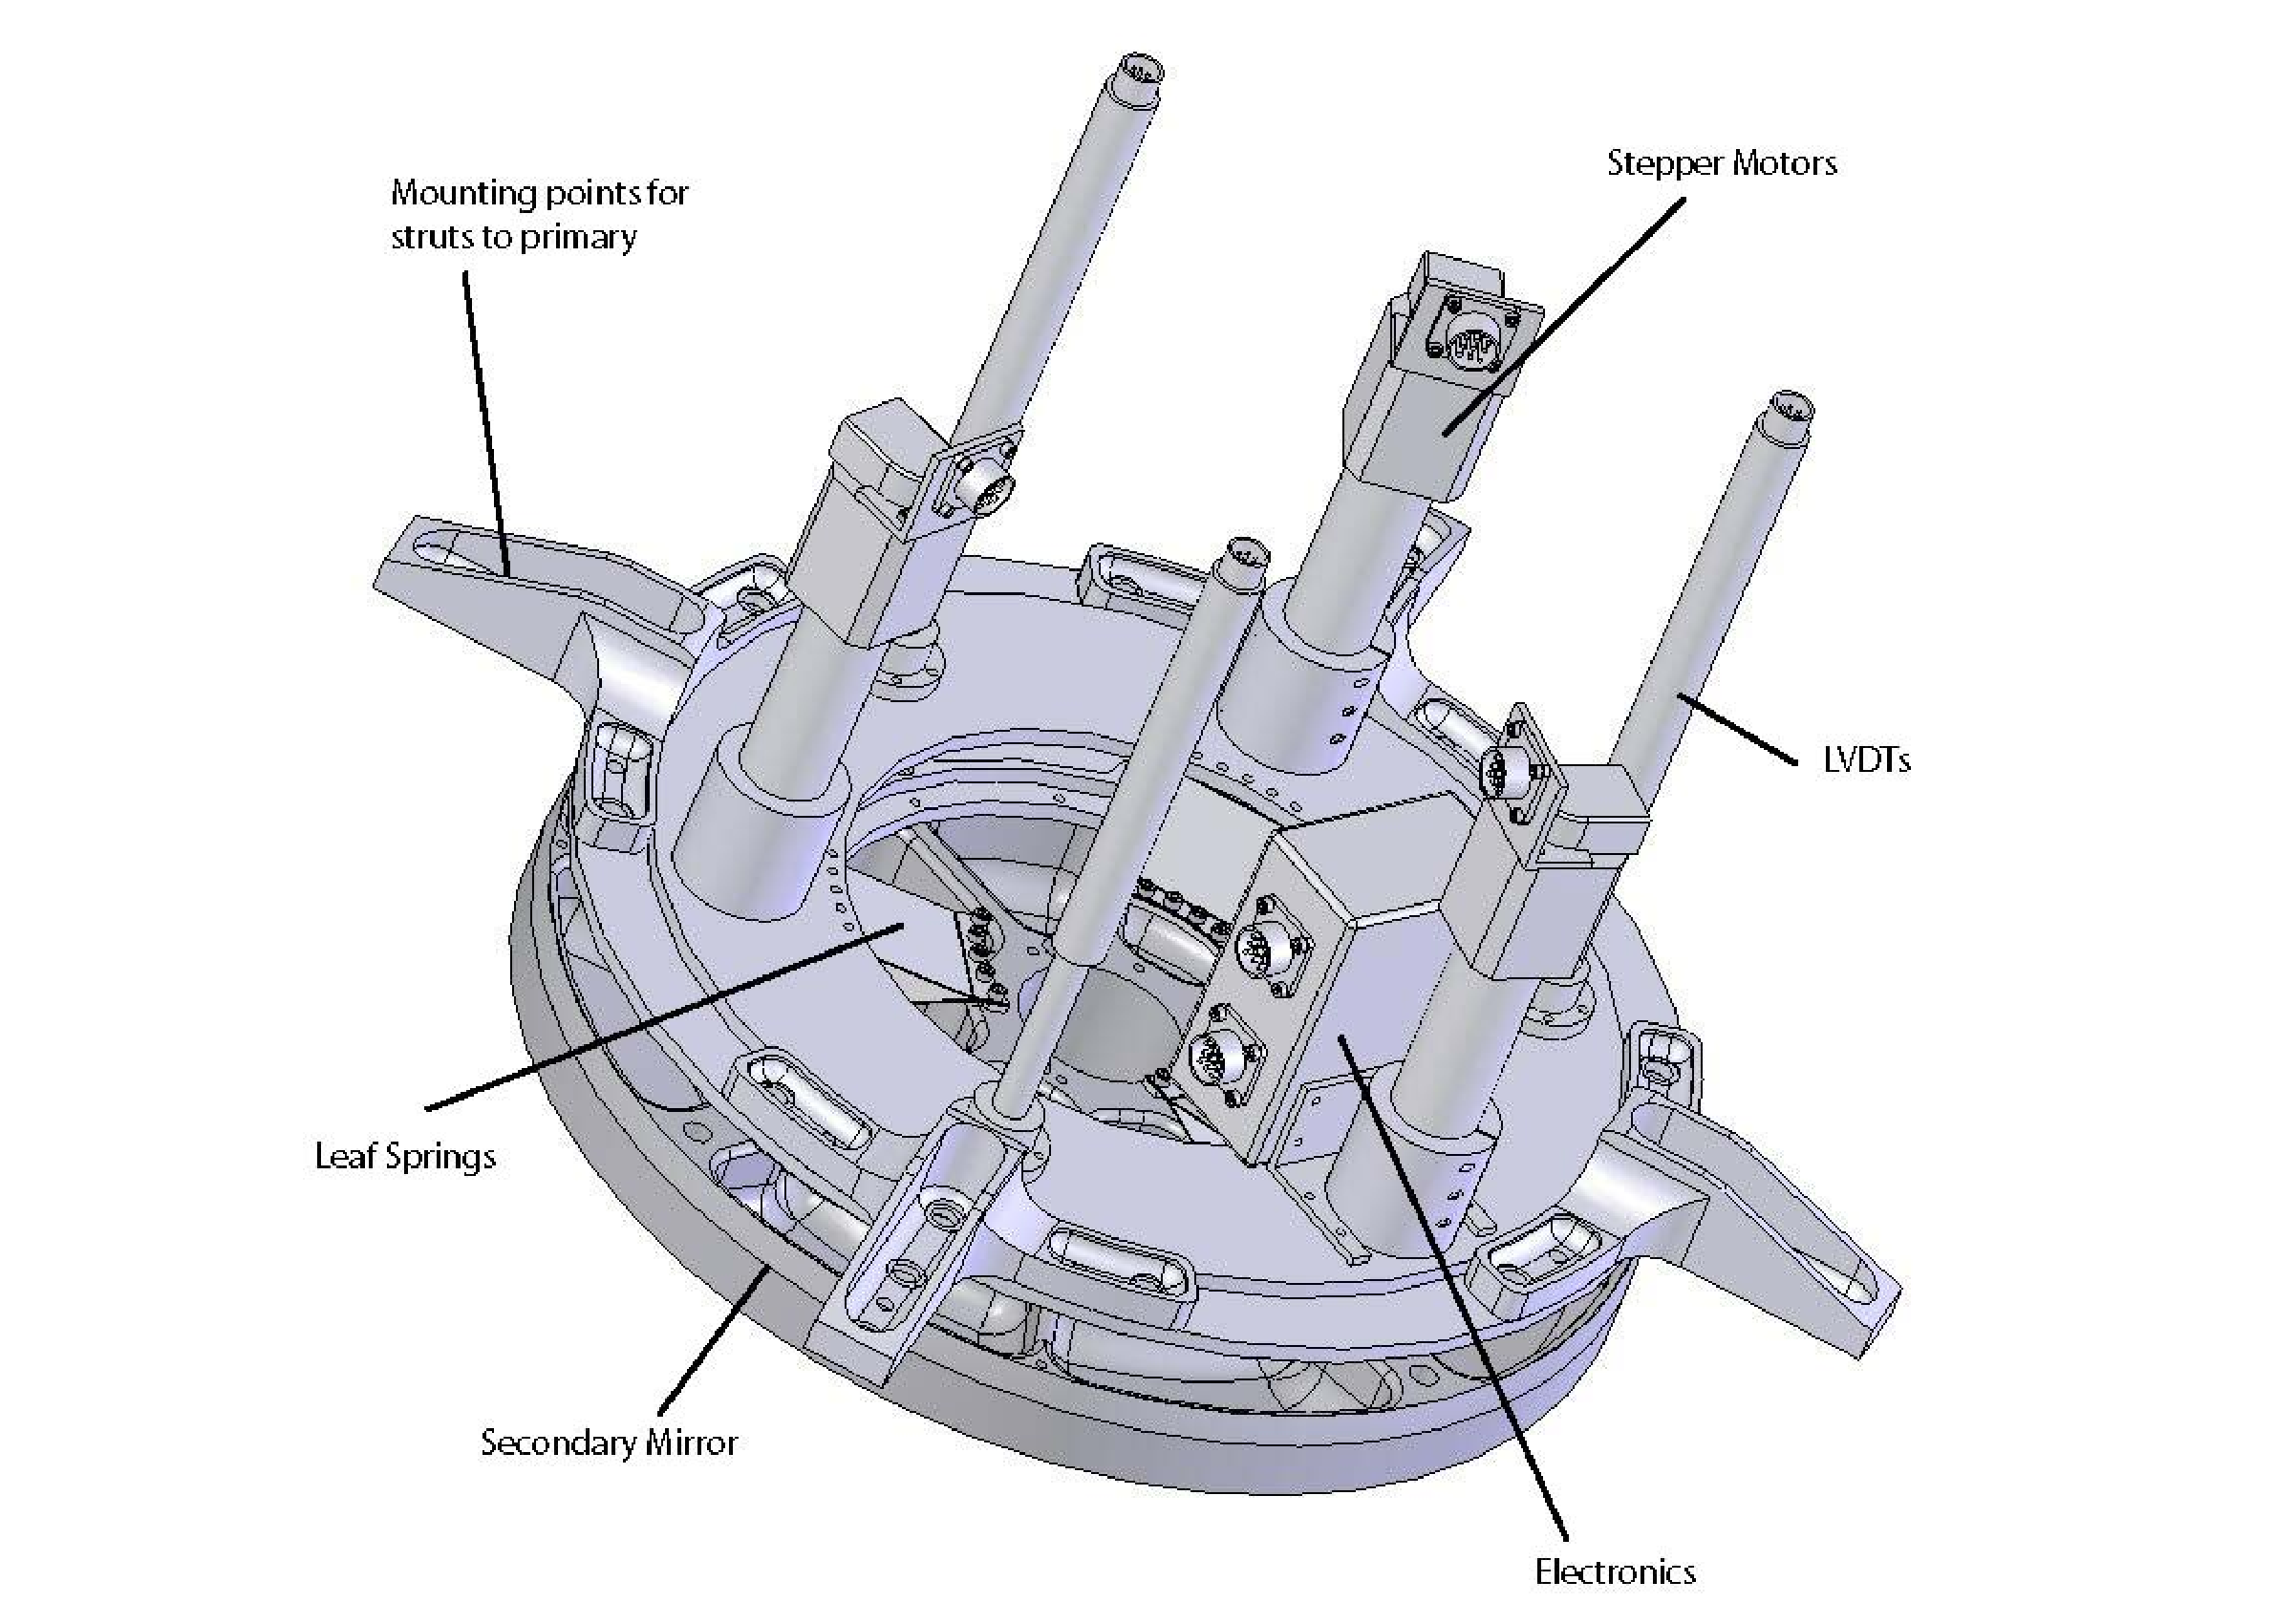
\psfig{file=secondary.pdf,angle=0, width=2.3in}
       \captionbaseline\caption {\small A rendering of the \blast\ secondary
	 positioning system.  \name\ will use the same system to
	 focus the off-axis secondary.  The system was successfully
	 tested during the \blast\ Antarctic flight in 2006.  It has
	 tip/tilt and positional accuracy (in one dimension) of
	 3~\mum.}
       \label{fig:SecondaryPositioning} 
     \end{center}
   \end{minipage}
 \end{tabular}
\end{figure}

\subsection{Cryogenics} 
\Responsible{Dicker, Devlin, Hailey-Dunsheath}{\color{red} \bf Need description of 1 K system; reviewers thought 15 psi referred to this system.  Need picture of spectrometer module in the cryostat.}
 
The \name\ receiver consists of an optical cavity inside a long hold-time liquid-nitrogen and liquid-helium cryostat.  We are copying the design from Super BLASTpol.  Both the nitrogen and helium are maintained at slightly more than 15~psi during the flight to minimize loss due to pressure drop at altitude.  A pumped pot maintains a 1~K stage with 20~mW of cooling power, which contains the entire spectrometer.  The detectors are cooled with a series of pumped $^3$He/$^4$He sorption fridges, which back a commercially available adiabatic demagnetization refigerator (ADR) to achieve a final temperature of 150 mK.
A two-stage $^3$He refrigerator (designed and manufactured at Penn) provides a
300~mK sink during flight with $30\,\mu$W of cooling power for 3~days.  It is backed and cycled by a $^4$He stage.  It can be recycled within
2~hrs.  Our groups have built over ten
receivers operating at temperatures from 50 to 300~mK, including an ADR for Z-Spec.

\subsection{Pointing and System} 
\label{sec:Observing} 

The \name\ gondola and pointing system is designed around the
successful \blast\ heritage.  The gondola is shown in Figure
\ref{fig:Gondola}.  It consists of a precision-pointed inner frame
(composed of the primary, secondary, near-field baffle, and cryostat)
supported by an external gondola.  The outer frame is pointed in
azimuth by a flywheel and an active pivot. The inner frame has an
elevation mount with direct-drive servo motors driving it relative to
the outer frame.  Balance of the inner frame is maintained by pumping
liquid from the bottom of the frame to the top to compensate for
cryogen boil-off.

The pointing system design is driven by the requirement of high
in-flight accuracy, with an absolute accuracy of half a beam, and
reconstructed accuracy $<$3\arcsec.  The \blast\ Antarctic flight
obtained a pointing reconstruction of $\approx 3$\arcsec\ at $1\sigma$
for small (1 degree) scans \Citep{pascale08}.  The absolute in-flight
pointing error was about 1\arcmin.  By improving the rigidity of the
inner frame, and by not requiring large motions, we expect to be able
to obtain better absolute in-flight pointing accuracy for \name.

The attitude determination system uses an array of pointing sensors
including two sophisticated star cameras, two sets of fast, low-drift
gyroscopes, a quad-GPS system, a digital Sun sensor, encoders, tilt
sensors, and a magnetometer.  The software is written to take full
advantage of the abilities of each sensor in a hierarchical scheme
where the fast, high-drift sensors (gyros) are continuously updated by
the slower, absolute sensors (star cameras) and is robust against
sensor failure.
%The software is capable
%of determining the quality of the data from each sensor and
%automatically shifts to the next available sensor if there is a
%problem.  
Optical encoders report the relative position of the inner frame to
the outer frame.  Motion sensing for the inner frame is provided by
two sets of three orthogonally-mounted, high bandwidth gyroscopes.

The absolute pointing sensors are two integrating star cameras
\Citep{rex06} that are mounted above the receiver on the inner frame.
Each star camera has an internal computer that calculates a real-time
pointing solution at 1~Hz by comparing measured star separations with
an on-board catalog of stars.  The cameras are capable of dead
reckoning.  The two cameras run independently, providing failsafe
redundancy.
%This redundancy provides a
%failsafe backup and continuously measures the precision of the star
%camera pointing solution.  
The camera system has been tested extensively on the ground and has
flown four times on balloon payloads (three times on \blast\ and once
on the x-ray telescope InFOC$\mu$S).  
%The star cameras can identify
%magnitude 8 stars with an integration time of 300~ms in typical
%daytime float conditions.  
A comparison of simultaneous pointing solutions from both cameras
gives an rms uncertainty of $<$2\arcsec.  To meet the absolute
pointing requirements for \name, we will reduce the field of view of
the cameras by a factor of two and use new CCDs with enhanced quantum
efficiency that roughly doubles the sensitivity in the far red (where
\name\ uses them).  This will allow us to obtain high-accuracy,
continuously updated pointing solutions for our observations.

% Results from a quick check of when we did an az el goto for a fridge cycle (10000 frames starting at 835200).  We only had the one star camera at this point, but it was working fairly well.
% 
% If I take Natalie's latest star camera solution and calculate the sigma for how much we bounced around I get ~3 arcsec in the elevation direction and ~10 in the cross elevation direction.  So that is a rough estimate of our precision.  Our accuracy (at least compared to the final pointing solution) was not as good: we were attempting to point at Az=50.7074, El=133.017.   If you look at the plot you can see that we appear to have been off by ~0.25 in Az and X-El.


\section{Flight Operations}
\label{sec:FlightOperations}

We plan for two North American flights, each overnight, with a maximum flight time of approximately 24 hours, during which science data will be primarily acquired during the night.  North American flights from Ft. Sumner, NM, or Palestine, TX, are typically scheduled in June or September to take advantage of ``turnaround'' wind conditions to produce the longest flight times.  The availability of scientific targets strongly favors June for flights of \name. In June 2016, the planets Mars, Saturn, and Jupiter are available at modest elevation for calibration.  The H-ATLAS fields at the NGP as well as GAMA12 and GAMA15 are available for pointed observations of lensed submillimeter galaxies in the early part of the night.  Further north, well-studied small deep fields such as GOODS-N and the Groth Strip are available for long integrations testing the intensity mapping and stacking analyses.

% In Figure \ref{fig:Observing}, we show the availability of various fields for both pointed and mapping observations, and the planets available for absolute calibration.

% \begin{figure}[h]
%   \begin{tabular}{ll}
%     \begin{minipage}{3.25in}
%       \begin{center}
% 	\includegraphics[width=3.25in]{observing_june2016.pdf}
% %{madau_plot_somerville08.pdf}
%       \end{center}     
%     \end{minipage} &
%     \begin{minipage}{3.25in}
%       \begin{center}
% 	\caption {\small The sky above New Mexico on 1 June 2016.  The planets Mars, Saturn, and Jupiter are available at modest elevation for calibration.  The H-ATLAS fields at the NGP as well as GAMA12 and GAMA15 are available for pointed observations of lensed submillimeter galaxies in the early part of the night.  Further north, well-studied small deep fields such as GOODS-N and the Groth Strip are available for long integrations testing the intensity mapping and stacking analyses.}
% 	\label{fig:Observing}
%       \end{center}
%     \end{minipage}
%   \end{tabular}
% \end{figure}

% \begin{figure}[h]
%     \begin{minipage}{6.5in}
%       \begin{center}
% 	\includegraphics[width=6.5in]{}
%       \end{center}
%     \end{minipage}
%     \caption {\small The sky above New Mexico on 1 June 2016.  The planets Mars, Saturn, and Jupiter are available at modest elevation for calibration.  The H-ATLAS fields at the NGP as well as GAMA12 and GAMA15 are available for pointed observations of lensed submillimeter galaxies in the early part of the night.  Further north, well-studied small deep fields such as GOODS-N and the Groth Strip are available for long integrations testing the intensity mapping and stacking analyses.}
% \label{fig:Observing}
% \end{figure}

% We plan for a mission length of two weeks, for a total time aloft of
% 504 hours.  We assume 2 hours per day are taken up with recycling of
% the $^3$He fridges and other overhead operations, and 10\% of the time
% is given to calibration and pointing observations.  This leaves 415
% hours to be divided between two one-square-degree fields, for an
% approximate integration time per field of $\sim$200 hours.

The best launch opportunities occur at sunrise.  We expect to be at float altitude at approximately 10 AM.  This will give us 8 hours to cycle the fridges, check the detectors, and verify the pointing.  The fridge hold times are sufficient that a single cycling at the beginning of the flight will hold for the entire flight.  
Science observations will begin at sunset.  We anticipate 10 - 12 useful hours of science observations, including some after sunrise, in our calculations.

To establish the pointing initially, we will observe planets or other bright targets to establish the offset between the star cameras and the submillimeter optics.  The accuracy of the mechanical alignment and the blind pointing solution from the star cameras should be better than 2\arcmin, allowing the target to appear in the FOV created by the $5\times5$ pixel array from the image slicer.  A co-add of the spectral pixels will create a continuum image with high S/N.  This offset will need to be periodically re-checked throughout the flight.  These bright sources will also calibration of the PSF and focus checks for the secondary mirror.

For pointed observations, the two star cameras provide updates at 1 Hz.  In between camera updates, the position is held based on the gyroscopes, the current generation of which on \blast\ have drifts of 1\arcsec/second.  We will use improved versions with only 0.05\arcsec/second drift, allowing extremely accurate maintained positions between star camera solution updates.  This accuracy will be used to hold the target with in the slicer FOV.  The inevitable small motions around the nominal pointing center are actually advantageous as they modulate the target signal.  The reconstructed position of the target within the focal plane will be better than a few arcseconds, allowing efficient coaddition of signal from the target.  The off-target pixels as well as telluric-line-dominated spectral channels will be used to remove any effects of time-varying atmospheric emission.

For mapping observations, we will use a scan strategy will be similar to that of \blast, with scans at fixed elevation while the FOV is moved back and forth in
azimuth.  The inner frame is then stepped to cover the entire field.
In this mode, the scanning modulation helps to separate atmosphere and instrument drift to recover large scales in the image.

\subsection{Scheduling}

The flight software for \name\ will be designed so that it can operate
%\icaris\ will function 
autonomously after launch.  However, because line-of-sight communication is maintained for the bulk of the flight, emergency changes can be implemented if necessary. The target fields
will be decided before the flight.  The autonomous scheduling system
(developed for \blast) will use schedule files that consist of a
sequential list of observations or actions as a function of the Local
Sidereal Time.  This system is robust against temporary system
failures because the telescope only needs to know the current time and
location to resume operation upon recovery.  Using a local sidereal
clock rather than a clock fixed in some time zone, it is possible to
account for purely astronomical visibility constraints (such as the RA
of the Sun and of the astronomical targets) using a static
description.

For every launch opportunity, six schedule files are generated, which account for 3 different cases flight latitude and longitude, and two cases of measured instrument senstivity.
%The
%latitude of the gondola can change by as much as $\sim 15^\circ$
%during a flight, hence three different schedules are created in
%latitude bands that are $5^\circ$ wide, with $1^\circ$ of overlap.
The gondola uses the GPS to decide which schedule file to use,
appropriate for the declination of the target field.  Two sets of
these three schedules are made: the first set assumes the instrument
is working with the target sensitivities; the second assumes
degradations of the telescope beam size by a factor of $\sqrt{2}$, and
sensitivity by a factor of 2.  At the beginning of the flight, the
sensitivities and beam size are estimated from scans across calibrators.  Based on this information the ground station team can decide which of the two
sets of schedule files the instrument should use, and switch between
the two using a single command.

\subsection{In-Flight Data Operations}

We will use several methods for primary calibration, most based on the
successful approaches used by the direct-detection millimeter-wave
spectrometer \zspec (e.g.,
\Citep{2010ApJ...722..668N,2011ApJ...731...83K}).  The \name\ bands
are sufficiently wide that a continuum calibrator can be used to
calibrate both the absolute and relative response of the channels, and
channels may also be co-added.  Absolute calibration can be checked againt the \herschel-SPIRE FTS measurements of the 
planets Mars \citep{swinyard10mars} and Saturn \citep{fletcher12}.

%Sources such as the red hypergiant
%star VY CMa, along with almost a dozen others, have been
%well-calibrated by \blast\ \Citep{truch09} and 

For frequency calibration we will begin with a Fourier transform
spectrometer (FTS) as a laboratory calibrator, as was done for \zspec.
\herschel\-SPIRE FTS observations of evolved stars 
\citep{groenewegen11,wesson11} such as NGC 7027.
%in bright, known redshift IRAS galaxies.  
A similar technique was used with
great success for \zspec\ using IRC+10216.  For \name, we have the additional
frequency calibration scale of line emission from the atmosphere
itself (since these lines will be narrow and do not suffer the severe
pressure broadening present in ground-based observations).

% Because \icaris\ can make a map of a pointing source, determining the
% offset between the star cameras and the instrument will be
% straightforward, similar to what was done for \blast.

The data rate from the \name\ detectors will be substantial, but not
prohibitive.  Each of the 6000 detectors will be sampled at a rate of
30 Hz, which, assuming 32 bit samples, is a rate of only 720 kB/s, or
2.6 GB per hour.  Over the course of a 24 hour flight, this results in
a total data volume of only $\sim70$~GB, including overheads for
housekeeping data.

%\pagebreak

\section{Plan of Work}

We recognize that \name\ will be a significant expense for the
balloon program.  In order to ensure that we are on-track with our
technology and on-schedule to achieve our goals, we will have
milestones and reviews by outside experts.  We will organize external
reviews of the two most critical and difficult aspects of the
instrument: the spectrometer optics (including configuration and
layout in the cryostat), and the detectors.

\subsection{Schedule}

\noindent{\bf GY1: Oct 2013 - Sep 2014:} Our first year will be
dominated by design and testing in preparation for Preliminary Design
Review (PDR) in May and a Critical Design Review (CDR) in September.
There will be separate PDRs and CDRs for the optics and detectors.
While this is an agressive schedule for these reviews, we need to
prepare for a launch in the 4th year of the work.

JPL has already done a considerable amount of work on the detectors.
%Their schedule of work is outlined in Figure \ref{fig:JPLSchedule}
An initial optics design has been completed. However, it will need to
be optimized and the details of laying out the optics, detectors, and
fridges in the cryostat which will need to be finalized.

% \begin{figure}[h]
%     \begin{minipage}{6.5in}
%       \begin{center}
% 	\includegraphics[width=6.5in]{ICARISSchedule2012.pdf}
%       \end{center}
%     \end{minipage}
%     \caption {\small JPL Schedule of Work}
% \label{fig:JPLSchedule}
% \end{figure}

\noindent{\bf GY2 - 3: Oct 2014- Sep 2016:} These years will be
dominated by building and testing all of the components of \name.
JPL will begin the production of the first detectors as well as the
detector package.  Penn will work with the contractors to complete the
telescope and gondola.  In addition we will construct the receiver,
cryogenics, and cold optics.  In the summer of 2016 we will integrate
the instrument and prepare for mission readiness review.

\noindent{\bf GY4: Oct 2016 - Sep 2017:} The first flight of \name\
is targeted for June 2017.  Data reduction software will be in place,
and reduction will begin promptly upon data acquisition.

\noindent{\bf GY5: Oct 2017 - Sep 2018:} The final year of the grant
is devoted to analysis of the data and a planned second flight in June 2017.  We have a strong track record in
analysis and releasing our data promptly to the community through the
NASA IPAC archive.\footnote{See, for example:\\ {\tt
http://irsa.ipac.caltech.edu/Missions/bolocam.html} and\\ {\tt
http://irsa.ipac.caltech.edu/Missions/blast.html}}

We have considered the reduction of risk throughout the process,
largely by drawing on the proven \blast\ heritage for the gondola and
pointing.  We also consider here
several contingencies and options for descope.  The \name
spectrometer design is highly modular.  This allows for the possiblity
of excluding one or more modules from the flight instrument if there
is a problem with the detectors or optics design.  The impact on the
science would be a reduction of the redshift range accessible.  

% The
% Antarctic flight is planned for GY4 Q4 (June 2017).  This leaves
% 1.5 years after recovery for data analysis.  However, should the
% schedule slip, a flight occurring in January 2017 would still provide
% 8 months for data analysis within the current grant.  As the
% additional year would also allow further development of the software,
% this should be sufficient, although we still target an earlier flight.

\subsection{Division of Labor and Personnel} 

To achieve the ambitious goals of this program, we have assembled a
group of scientists with the wide range of backgrounds necessary to
design, build and fly the instrument within the time scale described.
%,
%including key contributions from our international collaborators.  
Our
team includes world leaders in advanced submillimeter detectors,
background-limited (sub)millimeter spectroscopy, and scientific
ballooning.  Our team includes veterans from multiple balloon payloads
(notably \blast).% as well as suborbital rocket missions.  
We also have
extensive experience with millimeter-wave spectrometers (\zspec),
submillimeter receivers (ACT), and detector development (BLISS).  
%We
%have included theorists among our instrumental team to guide the
%design and speed the analysis of data.

The project planning is a group effort coordinated by the PI at the
University of Pennsylvania through frequent telecons and WWW-based
information exchange.  The University of Pennsylvania (Aguirre,
Devlin) will build the receiver, telescope and gondola.  JPL
(Bradford) will supply the detectors and detector mounts.  
%NIST will
%supply the cold multiplexing electronics.  The University of British
%Columbia (Halpern) will provide the multiplexing hardware for the
%detectors as well as crucial support for flight planning.  Cardiff
%(Pascale) will provide flight campaign and data analysis support, as
%well as cryogenic filters.  Cornell (Stacey) will provide oversight on
%scientific requirements.  Irvine (Cooray) will lead the theoretical
%work.  
All collaborators will share in the data analysis.  Close
collaboration between the experimentalists, theorists and observers in
our team will continue throughout the flight planning, field and
source selection, and the analysis of the data.  The entire team has
been involved with the successful analysis of several large, complex
CMB and submillimeter datasets and has an excellent history of prompt
publication and distribution of data.

%\subsubsection{Penn}
%
%Aguirre was PI (and C.~M.~Bradford co-PI) of NSF AST 0807990,
%``Broadband Millimeter Spectroscopy with \zspec: Molecular Diagnostics
%of Local ULIRGs and Redshifts for Submillimeter Galaxies'', which
%expired in June 2011.  This grant produced detailed studies of the
%local (U)LIRGs M82 \Citep{2010ApJ...722..668N} and NGC1068
%\citep{2011ApJ...731...83K}, as well as redshifts for high-$z$
%galaxies from the {\em Herschel} ATLAS and HerMES surveys
%\Citep{2010arXiv1009.5983L,2011ApJ...733...29S,2011ApJ...732L..35C,2011ApJ...738..125G}.
%These redshifts were essential in establishing the strongly lensed
%nature of the brightest {\em Herschel} sources, as reported in
%\citet{2010Sci...330..800N}.  Other exciting discoveries from Z-Spec
%also included the largest known mass of water around the quasar
%APM08279+5255 \citep{2011ApJ...741L..37B} and the discovery of water
%in other high-redshift star-forming galaxies
%\citep{2011A&A...530L...3O}.  
%
%Aguirre is also currently co-PI of NSF
%AST 1125558 ``Collaborative Research: Precision Array for Probing the
%Epoch of Reionization (PAPER)''.  PAPER is a dedicated attempt to
%detect the highly redshifted 21 cm emission from the epoch of
%reionization.
%
%The array
%is being constructed in the Karoo Desert of South Africa, near the
%South African SKA site, and since beginning operations there in
%October 2009, has reached 64 operational antennas, half its planned
%size.  Data of excellent quality is pouring in, and PAPER is on track
%for full science data in late 2012 or early 2013.  Aguirre has one
%student supported under this grant working on PAPER data
%analysis. Recent results from PAPER include a new southern sky point
%source catalog \citep{2011ApJ...734L..34J}, compiled by the PI's first
%graduate student, who defended in July 2011.  Considerable work has
%also gone into novel approaches to array configuration and power
%spectrum analysis \citep{2011arXiv1103.2135P}.  
%

%Co-I Devlin was the PI of \blast, together with co-I's Pascale and
%Halpern.  In December of 2006 \blast\ had an 11-day LDB flight in
%Antarctica.  \blast\ demonstrated our successful integration of the
%sensitive detector arrays and readout electronics, precision optics,
%accurate pointing system, careful flight planning, and finally,
%intensive data analysis.  BLAST has a produced a tremendous body of
%work, with more than twenty published papers (including one in Nature
%\Citep{devlin09}).  BLAST also produced a number of results on
%submillimeter galaxies which anticipated \herschel, including
%measurements of the galaxies' clustering \Citep{viero09}, number
%counts \Citep{patanchon09}, star formation history \Citep{pascale09},
%redshift distribution and luminosity function \Citep{eales09}, as well
%as the far-IR radio correlation \Citep{ivison10}, and the detection of
%strongly lensed sources by clusters \Citep{rex09}.  \blast\ was a
%fantastically successful project.  We hope to extend its legacy with
%\name.
%
%Toronto (Netterfield) will provide and support most of the updated
%electronics and data acquisition system.  They will also continue to
%be the main supporters of the flight software.  

 


%\input{section_results}

\begin{table}[th]
\caption{\name\ Instrument Parameters}
\label{tab:Parameters}
\center{
\begin{tabular}{l|c|c||c|c||l}

%and & $z_{mean}$ & Time per beam & $I_{\cii}$ & $P_{shot}$ & $P_N$ & S/N & \multicolumn{2}{c}{Detections} \\
%& & [hr] & [Jy~sr$^{-1}$] & \multicolumn{2}{c}{[\psu]} & & $>5\sigma$ & $>3\sigma$ \\
\hline
\multicolumn{6}{l}{\bf Telescope} \\
\hline
Temperature & \multicolumn{5}{l}{270K} \\
Diameter & \multicolumn{5}{l}{1.8~m} \\
Illumination & \multicolumn{5}{l}{0.93 (primary mirror is pupil stopped)}\\
Emissivity & \multicolumn{5}{l}{0.04} \\
Primary $f/\#$ & \multicolumn{5}{l}{1.25} \\
Ritchey-Chretien $f/\#$ & \multicolumn{5}{l}{5} \\
%Available FOV & \multicolumn{5}{l}{29\arcmin $\times$ 29\arcmin} \\
\hline
\multicolumn{6}{l}{\bf Detectors} \\
\hline
TiN \Tc & \multicolumn{5}{l}{0.9 K} \\
Base temperature & \multicolumn{5}{l}{250 mK} \\
%$d\ln{R}/d\ln{T}$ & \multicolumn{4}{c}{100} \\
%Heat Capacity & \multicolumn{4}{c}{300 fJ/K} \\
%$P_{saturation}/P_{absorbed}$ & \multicolumn{4}{c}{20} \\
%Thermal Conductivity & \multicolumn{4}{c}{2.4 / 1.6 pW/K} \\
KID resonator Q & \multicolumn{5}{l}{10$^5$}\\
KID resonant frequencies & \multicolumn{5}{l}{100--250~MHz}\\
MAKO pixel response & \multicolumn{5}{l}{$1.2\times10^{7}$ $(\delta f/f)\,\rm W^{-1}$, measured}\\
\name\ pixel response & \multicolumn{5}{l}{$4\times10^{8}$ $(\delta f/f)\,\rm W^{-1}$, scaled from MAKO as (volume)$^{-1}$ and \Tc$^{-2}$}\\
\Sxx (due to TLS) & \multicolumn{5}{l}{$1.0\times10^{-18}$ $(\delta f/f)^2\,\rm Hz^{-1}$, same as MAKO}\\
Detector efficiency w/ horns & \multicolumn{5}{l}{65\%} \\ 
Detector NEP (optical) & \multicolumn{5}{l}{$2.5 \times 10^{-18}$ W$/{\sqrt{{\rm Hz}}}$} \\
$P_{absorbed}$ & \multicolumn{5}{l}{9 / 6 fW} \\
Photon NEP & \multicolumn{5}{l}{$5.4 / 3.5 \times 10^{-18}$ W$/{\sqrt{{\rm Hz}}}$} \\
%$\rm{NEP}^2_{photon}/\rm{NEP}^2_{total}$ & \multicolumn{4}{c}{0.7 / 0.6} \\
%$\tau_{optical}$ & \multicolumn{4}{c}{11 / 16 ms} \\
\hline
\multicolumn{6}{l}{\bf Spectrometer} \\
\hline
Format & \multicolumn{4}{c}{2 modules, each $ 25~{\rm spatial} \times 64~{\rm spectral}$}\\
$R$ & \multicolumn{4}{c}{450 (670 km s$^{-1}$)} \\
Optical efficiency & \multicolumn{4}{c}{40\%, exclusive of horn and detector} \\
\hline
& \multicolumn{2}{c || }{Short Wavelength} &  \multicolumn{2}{c ||}{Long Wavelength} & \\
\hline
Wavelength range & 240 -- 276 & 276 -- 317 & 317 -- 365 & 365 -- 420 & \mum \\
$\Delta \nu$ & 2.58 & 2.25 & 1.95 & 1.70 & GHz \\
Beam FWHM & 25 & 29 & 34 & 39 & \arcsec \\
Slit FOV & 10.0 & 11.6 & 13.6 & 15.6 & \arcmin \\
NEI & 3.4 & 2.1 & 1.5 & 1.0 & $\E{7}$ \sbs \\
Line sensitivity & 1.58 & 1.13 & 0.92 & 0.71 & $\E{-17}$ W~m$^{-2}~\sqrt{\rm{sec}}$ \\
\hline
% \multicolumn{6}{l}{\bf Survey Parameters for 200 hr 1 square degree}\\
% \hline
% $z_{mean}$ & 0.63 & 0.88 & 1.16 & 1.48 & \\
% Time per beam & 0.19 & 0.25 & 0.33 & 0.44 & hr \\
% Beams per deg$^2$ & 17 & 13 & 9.7 & 7.3 & $\E{3}$ \\
% $I_{[CII]}$ & 8.27 & 9.68 & 8.22 & 3.72 & $\E{4}$ \sbu\\
% $P_{shot}$ & 1.34 & 1.55 & 1.44 & 1.02 & \multirow{2}{*}{$\E{9}$ \psu}\\
% $P_N$ & 523 & 347 & 274 & 164 & \\
% S/N & 590 & 926 & 1085 & 767 & \\
% $L_{[CII]}(5\sigma)$ & 3.11 & 1.88 & 1.34 & 0.891 & $\E{-18}$ W~m$^{-2}$\\
% Detections $>5\sigma$ & 50 & 20 & 10 & 5 & \\
% $L_{FIR}(5\sigma)$ &  1.3590 & 1.86 & 2.63 & 3.20 & $\E{12}$ \Lsun \\
% $L_{[CII]}(1\sigma)$ & 0.6215 & 0.3752 & 0.2674 & 0.1783& $\E{-18}$ W~m$^{-2}$\\
% Detections $>1\sigma$ & 2700 & 1000 & 700 & 500 & \\
% $L_{FIR}(1\sigma)$ & 2.72 & 3.72 & 5.25  & 6.40 & $\E{11}$ \Lsun \\
\hline
\end{tabular}
}
\end{table}

\clearpage

\newpage

\pagestyle{empty}

\bibliographystyle{unsrt_no_month}
%{astron}

%{astron}

\bibliography{master_references}

\newpage
\setcounter{page}{1}

% NASA PI biographical sketch
% Last updated 2012 March 22
% This is going to be an attempt to make a definitive version.  Sigh.
% It really needs to linked with a publications bibtex.

\parskip0pt
% -----------------------------------------------------------------------------
% This stuff changes very slowly
{\centering{\bf
James E. Aguirre

Professional Preparation}

}

\noindent\begin{tabular}{lll}
{Georgia Institute of Technology} & Physics / Applied Mathematics & BS 1997 \\
{University of Chicago} & Physics & PhD 2003 \\
{University of Colorado, Boulder} & Postdoctoral Research Associate & 2003 - 2005 \\
{National Radio Astronomy Observatory} & Jansky Postdoctoral Fellow & 2003 - 2008 \\
\end{tabular}

{\centering {\bf Appointments}

}\noindent {Assistant Professor}, Department of Physics and Astronomy, University of Pennsylvania, 2008 - \\ 
\noindent {Jansky Fellow}, National Radio Astronomy Observatory, 2005 - 2008 \\
\noindent {Postdoctoral Research Associate}, University of
Colorado, Boulder,2003 - 2005 \\
{Graduate Research Assistant}, University of Chicago, Department of Physics, 1997 - 2003 \\
\noindent {National Science Foundation Graduate Research
Fellow}, awarded 1997.
% -----------------------------------------------------------------------------

{\centering {\bf Projects and Grants}
 
} 
\begin{description}
\parskip0pt
\item
$\bullet$ PI of NSF Astronomy and Astrophysics Grant AST-0807990 ``Broadband Millimeter
Spectroscopy with Z-Spec: Molecular Diagnostics of Local ULIRGs and
Redshifts for Submillimeter Galaxies'', 7/1/2008 - 6/30/2011, \$426,977

\item
$\bullet$ PI of University of Pennsylvania Research Foundation Grant ``A
Cryogenic Testbed for Advanced Millimeter-Wave Astronomical
Detectors'', 7/27/2009- 6/31/2010, \$50,000

\item 
$\bullet$ PI of Mt. Cuba Astronomical Foundation Grant ``An Advanced Data
Handling System to Enable the Detection of the Epoch of
Reionization'',\$100,000

\item
$\bullet$ Co-I of NSF Astronomy and Astrophysics Grant AST-1007905 ``High Resolution
Observations of the Sunyaev-Zel'dovich Effect in Clusters of Galaxies
and High-z Galaxies at 90 GHz Using the GBT'' (PI M. Devlin) 7/1/2010
- 6/30/2012, \$545,561

\item
$\bullet$ Co-I and Executive Committee member for the NSF grant AST 1125558 ``Collaborative Research: Precision Array for Probing the Epoch of Reionization (PAPER)'', a joint venture with University of California Berkeley, and NRAO / University of Virginia

%\item
%Collaborator with the ACTpol

\end{description}

{\centering {\bf Relevant Publications}
 
} 
\begin{description}%{}{\itemindent=0pt}% \leftmargin=0pt}
\parskip0pt
% -----------------------------------------------------------------------------
% MUSTANG2
%\item \hornerAbell
%\item \limaCounts
%\item \masonRXJ
%\item \cottonRadioGalaxies
%\item \sayersBlindClusters
% -----------------------------------------------------------------------------

% -----------------------------------------------------------------------------
% BAOBAB / MWA-PAPER Sky Map
%\item \jacobsNewSource
%\item \lidzCOMapping
%\item \parsonsSensitivity
%\item \parsonsPAPEREight
%\item \carilliLymanAlpha
% -----------------------------------------------------------------------------

% -----------------------------------------------------------------------------
% SuperSpec / CSF
\item \bradfordAPMWater
\item \lidzCOMapping
\item \scottHERMES
\item \negrelloLenses
\item \bradfordCloverleaf
\item \kamenetzkyTenSixtyEight
\item \naylorMEightyTwo

% -----------------------------------------------------------------------------

\end{description}
{\centering {\bf Additional Publications}

}
\begin{description}%{}{\itemindent=-2pc}% \leftmargin=1pc}
\parskip0pt
% -----------------------------------------------------------------------------
%MUSTANG2

% -----------------------------------------------------------------------------

% -----------------------------------------------------------------------------
%BAOBAB / MWA-PAPER Sky Map
\item \aguirreBGPS
%\item \bradfordAPMWater
\item \limaCounts
%\item \negrelloLenses
%\item \cottonRadioGalaxies
% -----------------------------------------------------------------------------

% -----------------------------------------------------------------------------
%SuperSpec / CSF
\item \jacobsNewSource
\item \parsonsSensitivity
\item \parsonsPAPEREight


% -----------------------------------------------------------------------------

\end{description}
{\centering {\bf Synergistic Activities}

}
\noindent %$\bullet$ National Radio Astronomy Observatory K-band Focal
%Plane Array Critical Design Review Committee, January 2009 $\bullet$
%Contributor to science white papers submitted to US Astro2010 Decadal
%Survey 
$\bullet$ Reviewer for NASA Astrophysics Theory Program 2009
$\bullet$ Developed and taught a one week course in radio astronomy
for the Penn Summer Science Academy (PSSA), 2010 and 2011 $\bullet$
Public lectures to NRAO Pulsar Collaboratory and PSSA $\bullet$
Reviewer for MNRAS $\bullet$ US panelist for a scientific review
proposed instrument suite the Japanese satellite SPICA


%\newpage

%\input{section_jpl_sow}

\newpage

\begin{center}
{\bf \large Budget Justification}
\end{center}

This proposal asks for funds to design, build, and fly \name\ and
analyze its data.  
%Like \blast, we will accomplish much of what can be
%done from a satellite at a small fraction of the cost.  
We already have extensive infrastructure from \blast\ for support in the field.  The \name\ gondola and flight electronics are clones of the proven \blast\ design.  We believe it will take three years to design and build the payload
with overnight North American flights in the fourth and fifth year, with analysis promptly after the flights.  The total amount of data will be modest, and flying later will allow the reduction pipeline to be more fully developed.

A large fraction of our budget goes to JPL to design, develop and
build the detectors.  The \name\ detector development program will make possible a future balloon mission competitive with satellites, as well as  
provide dividends for future space missions and benefit the
community generally.  The Penn budget includes JPL as a subcontract;
however as a NASA center, these funds are allocated directly.  The JPL
budget is included as a separate spreadsheet.

% We have also included a subcontract to A. Cooray at University of
% California Irvine to provide support for the theoretical calculations
% necessary for successful scientific returns, and for assistance with
% the data analysis to ensure sufficient manpower to complete the
% analysis within the lifetime of this grant.

% \name\ will rely on the commitment and support from our foriegn
% collaborators.  %In particular, Enzo Pascale (Cardiff), and Mark
% Halpern (UBC) will be leading efforts at their home institutions.
% They are some of the most experienced people in scientific ballooning.
% Their expertise is highly sought after and we are fortunate to have
% them on our experiment.  In addition, they bring substantial resources
% in terms of people and equipment.  However, our plan does not rely on
% them receiving direct funding for
% \name.

\begin{itemize}
\item 
{\bf Personnel} We have a number of very experienced people working on
\name, and will train new postdocs and graduate students.

\begin{itemize} 

\item
Jeff Klein has functioned as the project scientist for \blast\ since
its inception.  He is universally accepted within the collaboration as
an indispensable member of the team.  His knowledge base supports the
entire project.  Through his work on ACT he has also become an expert
with the TES detectors and most importanly the multiplexing
electronics. He is supported 2 months/year on \name\ during the
final three years of the grant to support integration and field work.

\item
Simon Dicker has been a scientist at Penn for more than 10 years.  He
designed, built, and fielded the first array of bolometers on the
Green Bank Telescope. He has extensive experience with optical design
and TES detectors.  He is supported during the initial portion of the
award to work on optical and cryogenic design, and has already begun
designing the spectrometer and telescope optics.

\item
We will hire two postdocs at Penn to help design and build the many
new components for \name, as well as a postdoc through the JPL
subcontract
%, and on e through the Irvine contract.  
We have included
the biographical sketch of Steve Hailey-Dunsheath, who has 
%postdocs who have 
expressed an interest
in the proposal and contributed to it.
%(Lupu, Murphy, Hailey-Dunsheath,
%Gong, de Bernardis).  These are potential candidates for hire at one
%of Penn, JPL, or Irvine.

\item
There will be two new graduate students at Penn.  With the help of our
experienced staff and postdocs, these students will be coming up to
speed on the \name\ instrument to help support the next generation
of experiments.  They will also work on specialized data planning and
analysis.  Aguirre currently has one student who will help train the new students: Bade Uzgil, partially supported by a NASA GSRP has been
doing theoretical calculations in intensity mapping.

\item
Undergraduates have been involved with all of our projects (over 50 in
the last 10 years).  They have worked closely with our team to help to
build and support the instruments.  Most move on to graduate school.  Some
are even working on balloon payloads for other projects.  Support is
requested for one 40 hour-per-week undergraduate each summer.

\item
There is partial summer salary support for Aguirre and Devlin.
The JPL subcontract provides partial support to Bradford.

\item
For calculation of overhead, Modified direct cost = total direct cost -
equipment - tuition

\end{itemize}

\item
{\bf Travel.}  The travel budget for \name\ is dominated by the field travel for two one-month campaigns in Palestine or Ft. Sumner.
%Mission Readiness in Palestine
%(one month), and LDB flights from Antarctica and/or Sweden.  
We have
been in the field several times with our instruments and have experience
conserving resources (such as renting houses instead of
individual rooms in hotels).  
%In addition to the field travel for
%launch and recovery, funds are requested in years 1 - 3 for travel
In addition, there is the necessary travel back-and-forth between JPL and Penn for training and assistance with testing and
integration (cross-pollination of the postdocs and graduate students) and also during years 4 and 5 for collaborative work on data analysis.  We have estimated \$60,000
for domestic travel over the five years.  In addition, \$5,000 in
foreign travel is requested for travel to conferences to present results.

\item
{\bf Lab Supplies.}  This covers miscellaneous hardware and tools
required for construction and testing, as well as flight operations.
A total of \$60,000 over 5 years is requested, with higher amounts in years 3 and 4 for contingency in preparing for the first flight.

\item
{\bf Cryogens.}  These are for flight operations as well as
running multiple laboratory tests.  As much as possible, we will use
an existing closed-cycle cryogenic system (see Facilities and
Resources) to conduct cold tests and thus conserve cryogens.
Estimated costs are based on an inflation-adjusted average of \$10 per liquid liter, and a consumption rate of the cryostat of 100 liters on cooldown and 10 liters per day there after.  Thus, a two-week cooldown costs approximately \$1500, allowing for boiloff and transfer losses.   We request \$12,000 per year (8 two-week cooldowns) for each year we have the cryostat (years 2 - 5)


\item
{\bf Publication.}  
We expect to have a significant number of papers from our flight
within a short period after data collection, and so we have included
the cost of publications years 4 and 5 of the grant.  A total of
\$10,000 is requested, amounting to about four large publications.

\item
{\bf Subcontracts} There is a subcontract to JPL, with budget attached separately. The JPL award will be made directly from NASA.  

\item {\bf Equipment}

\begin{itemize}

\item
{\bf Cryostat.}  We have based the cost on the Z-Spec dewar, which has a 48-hour hold time and ample cryogenic volume for the spectrometer optics.  
It includes the cost for the He3/He4 fridges and magnetic shielding.  The housekeeping thermometry and optics are specified separately.
% The
% internal volume required for \name\ is larger than that for \blast,
% and we have scaled up the price accordingly.  
Total cost is
estimated at \$50,000.
% divided over three years to allow for design,
% major manufacturing, and inevitable modifications.

\item
{\bf Cryostat Electronics.}  This includes cryogenic housekeeping thermometers and cables,  and their readout electronics, based on the \blast\ design and
experience.  No significant change is anticipated over the \blast\
budget, so we have simply reproduced the request, \$60,000.

\item
{\bf Adiabatic Demagnetization Refrigerator (ADR)}.  This provides the final stage of cooling of the detectors to 160 mK.  The cost of \$60,000 is based on a commercially available system quoted by High Precision Devices, Inc (HPD) in Boulder, Colorado. 

% \item
% {\bf Cryogenic Cable Harness.}  This is the cryogenic cabling not
% supplied as part of the JPL subcontract.  These cables will be almost
% exact duplicates of the ones used on ACT.  This will save on design
% costs, but they are still expensive to purchase from TekData in the
% UK, at an estimated cost of \$25,000.

\item
{\bf Pointing Electronics.} This includes all of the electronics to
run the gondola.  There are two computers, power distribution,
pointing sensors and star cameras, and interface boards to the motors and pointing
sensors.  Again, this is based on the \blast\ design, which will be
replicated, at a cost of \$60,000.

\item
{\bf Gondola.}  We will re-use the \blast\ 2010 gondola.  The cost here (\$10,000) is for a new inner frame to support the larger, heavier off-axis mirror.

\item
{\bf Gondola Motors.}  The \blast\ drive motors will need to be
redesigned for the larger mass and moment of the \name\ primary
mirror and cryostat, at an estimated cost of \$30,000.

\item
{\bf Primary Mirror.}  The primary mirror cost is based on a detailed estimate by
Magna Machining using a SolidWorks model of our current design, and including tolerance requirements.  The \$400,000 cost includes material, lightweighting machining, and surface cutting and polishing of {\it two} 2.5-meter off-axis mirrors.  Because the surface cutting is done on a vertical lathe, both mirrors can be cut simultaneously.  The second mirror provides a spare without significantly increasing the cost.

\item
{\bf Secondary Mirror.}  This is for the secondary mirror and
positioning system.  This is a nearly exact clone of the \blast\
design, and is costed accordingly.  Costs include the machining of the
mirror surface and lightweighting for the mirror, as well as the
focus-adjust mount for the mirror, its linear actuators, and the
electronics, estimated at \$50,000.

\item
{\bf Cold Optics.}  This is for the machining of the cold image slicing and relay optics, the diffraction gratings, the blocking filters, their support stuctures, and the mechanism for moving the grating.  The optical design calls for two spectrometer modules, each fed by an image slicer.  
Each spectrometer module has two mirrors (4 total), all of which are powered.  The surface accuracy of these mirrors can be
achieved with a machining process, and the largest of them is $\sim$20
cm.  In addition, there are two blazed diffraction gratings.  Based
on experience with the ZEUS spectrometer, the gratings are available
commercially at an expected cost per grating of approximately
\$15,000, and for mirrors of similar size and accuracy, the typical
cost is \$3,000 - \$5,000, depending on size, averaging about \$4,000.  Each module also requires positioning and alignment structures.  We estimate a combined cost of \$62,000 for both spectrometer modules.  The image slicing optics are much smaller, but require high alignment precision.  Combined with the necessary mounting hardware, we estimate \$25,000 for each slicer, for a total of 
\$112,000.

\item {\bf Lenslet Arrays}  These are the silicon lenses for focusing light on the KIDs.  Four are required, one for each array, from  VeldLaser at \$2000 each (as scaled from our prototype), for a total of \$8,000.

\item 
{\bf Detector Readout Electronics}
This is the frequency multiplexed readout for the kinetic inductance detectors (KIDs).  The cost includes \$14,000 for 4 SiGe amplifiers from Sandy Weinreb at Caltech (\$3.5k each), \$10,000 for 4 sets of cryogenic coaxial cable (\$2.2k for 2 NbTi runs (for $T<4$~K) and \$300 for 2 stainless runs), \$22,000 for the ROACH  electronics (two systems, each handling 2 readout chains).  Each ROACH system consists of: ROACH-1 board (\$2500), XC5VSX95T FPGA (\$2250), iStar chassis (\$515), ADC / DAC combo cards from Rick Raffanti (\$2650), and a readout computer (\$3000) which also handles data storage.  The total cost of the readout system is \$48,000.

% \item
% {\bf Detector Readout Electronics.}  These are the non-cryogenic
% electronics for driving the detector readout SQUID multiplexing
% (``mux'') system.  They will be supplied and supported by Mark
% Halpern's group at University of British Columbia.  The designs are
% based on those in operation on several experiments.  The mux scheme
% uses chip-select within the cryostat.  Each box is capable of reading
% out $32 \times 50 = 1600$ detectors, or enough for one of the $24
% \times 64 = 1536$ spectrometer modules.  The cost for one MCE box is
% \$75,000.  This is a complete system, including power supplies,
% control computer, fiber optics and cables, extension cards,
% MDM-connector breakout cards, and software and firmware support.  In
% addition, there is a one-time, non-recoverable engineering cost of
% developing the new firmware for chip-select addressing of \$8,000.
% The total is thus \$308,000. The budget is allocated so that 25\% of
% the system and its NRE are provided in the first year for the initial
% round of detector construction at JPL, with 25\% in the second year,
% and the remaining 50\% in year 3 prior to full delivery.
% 
% \item
% {\bf NIST Multiplexing Electronics} These are the cryogenic
% first-stage and series array SQUID amplifiers.  \name's 6144 pixels
% will be divided into 94 columns, each composed of 6 11-channel mux
% chips, for a total of $6 \times 94 = 564$ chips. At \$825 per chip,
% this comes to \$465,300.  The 94 columns require 94 series-array
% SQUIDs, Nyquist and bias chips, and Nb magnetic shielding modules.
% The series array SQUIDs are \$28,200, Nyquist and bias chip
% \$53,300, and the modules \$10,600, for a total of \$557,400.  The budget 
% is allocated so that 25\% of the system is provided in the first year
% for the initial round of detector construction at JPL, with 25\% in
% the second year, and the remaining 50\% in year 3 prior to full
% delivery.


% \item
% {\bf Solar Panels.}  We will purchase the same solar panels that we
% used on \blast, at a cost of \$25,000.

\end{itemize}

\end{itemize}


\newpage



\centerline{\bf Summary of Personnel Commitments and Costs}
\vspace{1in}



\begin{table}[tbh]
\begin{center}
\protect\small 
\vspace{1ex}
\begin{tabular}{lccccccc}
\hline \hline
Individual	&   &  & FY12 & FY13 & FY14 & FY15 & FY16  \\
\hline \\[-0.5ex]

J. Aguirre	   & Penn    &	&  0.35 / 0.08 &  0.35 / 0.08 &  0.35 / 0.08 &  0.35 / 0.08 &  0.35 / 0.08  \\
M. Devlin	   & Penn    &	&  0.20 / 0.04 &  0.20 / 0.04 &  0.20 / 0.04 &  0.20 / 0.04 &  0.20 / 0.04  \\
J. Klein	   & Penn    &	&  0.00 / 0.00 &  0.00 / 0.00 &  0.17 / 0.17 &  0.17 / 0.17 &  0.17 / 0.17  \\
S. Dicker	   & Penn    &  &  0.33 / 0.33 &  0.33 / 0.33 &  0.33 / 0.00 &  0.00 / 0.00 &  0.00 / 0.00  \\
Postdoc 1	   & Penn    &	&  1.00 / 1.00 &  1.00 / 1.00 &  1.00 / 1.00 &  0.00 / 0.00 &  0.00 / 0.00  \\
Postdoc	2	   & Penn    &	&  0.00 / 0.00 &  0.00 / 0.00 &  1.00 / 1.00 &  1.00 / 1.00 &  1.00 / 1.00  \\
Graduate Student 1  & Penn    &	&  1.00 / 1.00 &  1.00 / 1.00 &  1.00 / 1.00 &  1.00 / 1.00 &  1.00 / 1.00  \\
Graduate Student 2  & Penn    &	&  1.00 / 1.00 &  1.00 / 1.00 &  1.00 / 1.00 &  1.00 / 1.00 &  1.00 / 1.00  \\


%M. Bradford 	  & JPL      &	&  0.20 / 0.10 &  0.20 / 0.05 &  0.20 / 0.05 &  0.20 / 0.05 &  0.20 / 0.10  \\
%M. Kenyon	  & JPL	     &	&  0.50 / 0.50 &  0.50 / 0.50 &  0.25 / 0.25 &  0.00 / 0.00 &  0.00 / 0.00  \\
%T. Turner 	  & JPL	     &	&  0.00 / 0.00 &  0.00 / 0.00 &  0.75 / 0.75 &  0.50 / 0.50 &  0.05 / 0.05  \\
%Technician	  & JPL	     &	&  0.00 / 0.00 &  0.05 / 0.05 &  0.25 / 0.25 &  0.15 / 0.15 &  0.00 / 0.00  \\

% M. Halpern       & UBC    &  &  0.08 / 0.00 &  0.08 / 0.00 &  0.08 / 0.00 &  0.08 / 0.00 &  0.08 / 0.00  \\
% 
% G. Stacey       & Cornell    &  &  0.08 / 0.00 &  0.08 / 0.00 &  0.08 / 0.00 &  0.08 / 0.00 &  0.08 / 0.00  \\
% 
% E. Pascale	& Cardiff    &  &  0.08 / 0.00 &  0.08 / 0.00 &  0.08 / 0.00 &  0.08 / 0.00 &  0.08 / 0.00  \\

%B. Netterfield  & Toronto    &  &  0.35 / 0.00 &  0.35 / 0.00 &  0.35 / 0.00 &  0.35 / 0.00 &  0.35 / 0.00  \\
%Graduate Student& Toronto    &  &  1.00 / 0.00 &  1.00 / 0.00 &  1.00 / 0.00 &  1.00 / 0.00 &  1.00 / 0.00  \\
%Graduate Student & Toronto   &  &  1.00 / 0.00 &  1.00 / 0.00 &  1.00 / 0.00 &  1.00 / 0.00 &  1.00 / 0.00  \\

%P. Ade		& Cardiff    &  &  0.05 / 0.00 &  0.05 / 0.00 &  0.05 / 0.00 &  0.05 / 0.00 &  0.05 / 0.00  \\

%P. Mauskopf     & Cardiff    &  &  0.05 / 0.00 &  0.05 / 0.00 &  0.05 / 0.00 &  0.05 / 0.00 &  0.05 / 0.00  \\
%P. Hargrave	& Cardiff    &  &  0.05 / 0.00 &  0.05 / 0.00 &  0.05 / 0.00 &  0.05 / 0.00 &  0.05 / 0.00  \\
%C. Tucker	& Cardiff    &  &  0.05 / 0.00 &  0.05 / 0.00 &  0.05 / 0.00 &  0.05 / 0.00 &  0.05 / 0.00  \\
%S. Eales	& Cardiff    &  &  0.05 / 0.00 &  0.05 / 0.00 &  0.05 / 0.00 &  0.05 / 0.00 &  0.05 / 0.00  \\
%Graduate Student & Cardiff   &  &  1.00 / 0.00 &  1.00 / 0.00 &  1.00 / 0.00 &  1.00 / 0.00 &  1.00 / 0.00  \\

%M. Halpern      & UBC        &  &  0.08 / 0.00 &  0.08 / 0.00 &  0.08 / 0.00 &  0.08 / 0.00 &  0.08 / 0.00  \\
%Graduate Student  & UBC	     &  &  1.00 / 0.00 &  1.00 / 0.00 &  1.00 / 0.00 &  1.00 / 0.00 &  1.00 / 0.00  \\

\\
TOTAL                      & &  &  3.88 / 3.45 &  3.88 / 3.45 &  5.05 / 4.62 &  3.72 / 3.29 &  3.72 / 3.29  \\
\hline
\end{tabular}
\end{center}
\end{table}

\vspace{0.5in}
\noindent
This table summarizes the time commitments of personnel contributing
to this project in fractions of a year, {\it exclusive of JPL}.  For this, see their itemized budget.  The
first number in each fiscal year column indicates the time commitment
available for this work.  The second gives the amount supported by
this proposal.  These numbers refer to a schedule that includes
teaching and administrative duties.

\newpage



\newpage

%\input{BradfordCPSupport}

\newpage

\begin{center}
{\bf \large Facilities, Equipment and Other Resources}
\end{center}
\medskip
\noindent{\bf \large Penn}

%\begin{itemize}

{\it Existing Designs, Instrumentation and Equipment.}  \name\ will
rely heavily on existing designs and instrumentation from \blast, ACT,
and other projects.  Whenever possible we will share equipment with
\blast.  This includes systems such as the star cameras and other pointing 
sensors.  We also have complete laboratory and field supplies that
will be used for \name.\\

{\it Laboratory.} The University of Pennsylvania is equipped with a
high bay facility in which \blast-pol is currently undergoing
integration.  This facility will be sufficient for the integration of
the \name\ gondola.  Between Profs. Aguirre and Devlin there is
approximately 1,800~ft$^2$ of space allocated for this work and can
use 600~ft$^2$ more if necessary.  All of the rooms are plumbed for a
vacuum system and compressor.  The ceilings have hard attachment
points to mount 2-ton hoists.  One of the rooms is accessible by
fork-lift from the loading dock to move large pieces of equipment.\\

{\it Shops.} The physics department machine shop at Penn will be used
to manufacture most of the parts.  A CNC milling machine and lathe are
available with a skilled machinist.  The electronics lab at Penn is
extremely knowledgeable and their services can be made available as
needed.\\

{\it Computation and Data Storage.}  Aguirre maintains the central
computer cluster for PAPER data analysis and archival at Penn.  This
consists of 16 high-speed compute nodes as well as $>100$~TB of
storage.  This facility will be upgraded over the next two years as
part of NSF grant AST 1125558 ``Collaborative Research: Precision
Array for Probing the Epoch of Reionization (PAPER)'', at no cost to
this grant.  The computational needs of \name\ are minor compared to
the resources available from this shared resource.

The following equipment at Penn will be available for use on this
project:

\begin{itemize}

\item 
{\it Dedicated test cryostat} A cryostat with pulse-tube cooler,
$^4$He and $^3$He sorption fridges, and instrumentation will be
available for testing detectors and other cryogenic tests to avoid the
unnecessary use of liquid cryogens in the flight cryostat.

\item
{\it Cryogenic equipment.} Considerable infrastructure for supporting
cryogenic measurements exists and are ready to be dedicated to this
project.

\item 
{\it Infrared Fourier Transform Spectrometer.} This was built at Penn
by undergraduates and graduate students. It operates from 80~GHz to
1.2~THz and will be used to characterize the \name\ bandpass
response.

%\item {\it Other Resources.}  The Cardiff group will provide all of the
%filters needed for this work.  

\item {\it Standard laboratory test equipment} 

\end{itemize}

\pagebreak

\noindent{\bf \large Caltech}

We have access to a 600-square-foot laboratory space which is earmarked for this work.   We have a dedicated cryostat fitted with coaxial leads and cooled to 300 mK with a combination of a 4-K Cryomech pulse tube refrigerator and a Chase $^3$He cooler.   For initial measurements as our new readout is under development,  we also have access to HEMT amplifiers (LNAs), a vector network analyzer (VNA), a 0--40~GHz frequency synthesizer, preamplifiers, IQ demodulators, digitizers and a data acquisition computer.  These components allow the readout of a
single channel using a standard homodyne detection technique. 

For spectral profile measurement, we have both a long-throw ($\delta\nu$=300~MHz) Fourier-transform spectrometer as well as tunable local-oscillator sources for all frequencies throughout our range.

Finally, we have a millimeter / submillimeter wave beam mapper formed from a chopped thermal source on a 2-D raster stage.


%
%
%Dr. Peter Day (PI) maintains two highly instrumented dilution refrigerators dedicated to
%superconducting detector research. The first is a Janis Inc. conventional "wet" dilution
%refrigerator which is instrumented with SQUID amps, microwave LNAs, and an in-situ
%temperature controlled black body which can characterize the performance of both TES and
%MKID type detectors.  A second cryogen free or "dry" dilution refrigerator from Leiden
%Cryogenics has recently been commissioned. This refrigerator is currently operating with six
%sets microwave transmission lines and LNAs for testing of detectors with microwave readouts. In
%addition, the latter unit has a probe insert which can be introduced into cold space of the
%refrigerator from room temperature while operating the refrigerator. This will enable fast
%turnaround measurements.  A network analyzer, microwave frequencies synthesizers and related components are available for device characterization.
%

\paragraph{Superconducting Device Fabrication at the Jet Propulsion
Laboratory Microdevices Laboratory (MDL).}

Dr H.G.\ `Rick' LeDuc and his group at JPL maintains several sputter systems for
the sputtering of high-quality superconducting films including Nb,
Mo, Au, Ti, and Al and SiO2 films.  There are Unaxis Shutteline
chlorine and fluorine inductively-coupled plasma (ICP) etchers in
MDL for etching metal and dielectric films.

%MDL has a 0.25\micron resolution Cannon FPA 300 EX stepper with a 50
%nm alignment tolerance essential for defining the small features in
%our proposed TES bolometer design.  A JEOL 9300 electron beam writer
%is available to fabricate the wire mesh absorber of the bolometer.

Key lithographic tools within the Microdevices Laboratory (MDL)
include a Canon FPA300-EX3 projection stepper and a JEOL JBX-9300 FS
electron beam writer. The stepper has a 0.6 numerical aperture and a
KrF eximer laser light source (248nm) giving a resolution of 0.25
\micron and a high throughput rate. The electron beam writer has a
field emission source and a 100kV accelerating potential producing a
nominal 4nm electron beam diameter and nominal 20nm lines.  These
tools can be operated in a complementary mode in which the highest
resolution patterns are written by the e-beam tool and matched with
lower resolution patterns exposed by the stepper to maximize wafer
throughput.

\paragraph{Computing.} We have access to Caltech Astronomy Data Processing Facility, which hosts and maintains licenses for
various electromagnetic simulation and data analysis software such as L-Edit, HFSS, Sonnet,
ADS, IDL, and Matlab. We have included the cost for accounts and software licensing in our
budget.

%\subsection{MKID Test Facilities at JPL}

% The superconducting bolometer group centered at JPL's Microdevices
% Laboratory (MDL) specializes in the fabrication of low-T$_c$
% superconducting devices.  The group has extensive experience with
% low-T$_c$ materials and tunnel junctions, and is internationally
% recognized as the preeminent group for fabrication of superconducting
% mixer devices, having produced a number of important breakthroughs in
% materials and device technology for these applications.
% 
% The group has state-of-the-art facilities enabling in-house
% fabrication of membrane-isolated TESs from bare Si wafers to working
% devices.  Specific facilities include:\begin{itemize}
% 
% \item{A Tystar low-pressure chemical vapor deposition (LPCVD) system for 
% growing sub-micron $\rm Si_xN_y$ films on Si wafers.}
% 
% \item{Several systems for sputtering high-quality superconducting films of 
% materials such as Nb, Mo, Au, Ti, Al, as well as SiO2 films.}
% 
% \item{Unaxis Shutteline chlorine and fluorine inductively-coupled plasma 
% (ICP) etchers for etching metal and dielectric films.}
% 
% \item{State of the art lithographic tools, including a Canon FPA300-
% EX3 projection stepper and a JEOL JBX-9300 FS electron beam writer.
% The stepper has a 0.6 numerical aperture and a KrF eximer laser light
% source (248~nm) giving a resolution of 0.25~$ \rm\mu m$ and a high
% throughput rate. The electron beam writer has a field emission source
% and a 100~kV accelerating potential producing a nominal 4~nm electron
% beam diameter and nominal 20~nm lines. These tools can be operated in
% a complementary mode in which the highest resolution patterns are
% written by the e-beam tool and matched with lower resolution patterns
% exposed by the stepper to maximize wafer throughput}
% 
% \item{A Surface Technologies Systems deep-trench Si etcher to perform
% back-side anisotropic etching of the bolometers. Front side releases
% can be performed using a XeF$_2$ etcher.}
% 
% \end{itemize}
% 
% The JPL group also makes use of a number of cryogenic test facilities,
% which are available to this proposal at no cost:
% \begin{itemize}
% \item
% {A Janis JDR-100 $^3$He-$^4$He dilution refrigerator (DR) which
% reaches a base temperature of $<10~\rm\,mK$, and includes a
% temperature-controlled blackbody source for optical characterization.
% This cryostat is outfitted with four SQUID controller / readout
% channels, all filtered to eliminate RF injection to enable low-NEP
% testing.}
% 
% \item
% {A Janis Adiabatic Demagnetization Refrigerator (ADR) equipped with
% $8\times 32$-channel time domain NIST SQUID multiplexer (MUX chips at
% 1~K, cryogenic cabling, room-temp control electronics).}
% 
% \item
% {A Cryogen-Free testbed 50 mK testbed with an optical port has been
% procured and is under construction.  It will be compatible with the
% SQUID TDM, and will be used to demonstrate performance of the arrays
% before delivery to Philadelphia.} 
% 
% \end{itemize}

\end{document}

\end{document}


